% Generated by Sphinx.
\def\sphinxdocclass{report}
\documentclass[letterpaper,10pt,english]{sphinxmanual}
\usepackage[utf8]{inputenc}
\DeclareUnicodeCharacter{00A0}{\nobreakspace}
\usepackage[T1]{fontenc}
\usepackage{babel}
\usepackage{times}
\usepackage[Bjarne]{fncychap}
\usepackage{longtable}
\usepackage{sphinx}
\usepackage{multirow}


\title{ABCE Documentation}
\date{June 28, 2013}
\release{0.3.1alpha}
\author{Davoud Taghawi-Nejad}
\newcommand{\sphinxlogo}{}
\renewcommand{\releasename}{Release}
\makeindex

\makeatletter
\def\PYG@reset{\let\PYG@it=\relax \let\PYG@bf=\relax%
    \let\PYG@ul=\relax \let\PYG@tc=\relax%
    \let\PYG@bc=\relax \let\PYG@ff=\relax}
\def\PYG@tok#1{\csname PYG@tok@#1\endcsname}
\def\PYG@toks#1+{\ifx\relax#1\empty\else%
    \PYG@tok{#1}\expandafter\PYG@toks\fi}
\def\PYG@do#1{\PYG@bc{\PYG@tc{\PYG@ul{%
    \PYG@it{\PYG@bf{\PYG@ff{#1}}}}}}}
\def\PYG#1#2{\PYG@reset\PYG@toks#1+\relax+\PYG@do{#2}}

\def\PYG@tok@gd{\def\PYG@tc##1{\textcolor[rgb]{0.63,0.00,0.00}{##1}}}
\def\PYG@tok@gu{\let\PYG@bf=\textbf\def\PYG@tc##1{\textcolor[rgb]{0.50,0.00,0.50}{##1}}}
\def\PYG@tok@gt{\def\PYG@tc##1{\textcolor[rgb]{0.00,0.25,0.82}{##1}}}
\def\PYG@tok@gs{\let\PYG@bf=\textbf}
\def\PYG@tok@gr{\def\PYG@tc##1{\textcolor[rgb]{1.00,0.00,0.00}{##1}}}
\def\PYG@tok@cm{\let\PYG@it=\textit\def\PYG@tc##1{\textcolor[rgb]{0.25,0.50,0.56}{##1}}}
\def\PYG@tok@vg{\def\PYG@tc##1{\textcolor[rgb]{0.73,0.38,0.84}{##1}}}
\def\PYG@tok@m{\def\PYG@tc##1{\textcolor[rgb]{0.13,0.50,0.31}{##1}}}
\def\PYG@tok@mh{\def\PYG@tc##1{\textcolor[rgb]{0.13,0.50,0.31}{##1}}}
\def\PYG@tok@cs{\def\PYG@tc##1{\textcolor[rgb]{0.25,0.50,0.56}{##1}}\def\PYG@bc##1{\colorbox[rgb]{1.00,0.94,0.94}{##1}}}
\def\PYG@tok@ge{\let\PYG@it=\textit}
\def\PYG@tok@vc{\def\PYG@tc##1{\textcolor[rgb]{0.73,0.38,0.84}{##1}}}
\def\PYG@tok@il{\def\PYG@tc##1{\textcolor[rgb]{0.13,0.50,0.31}{##1}}}
\def\PYG@tok@go{\def\PYG@tc##1{\textcolor[rgb]{0.19,0.19,0.19}{##1}}}
\def\PYG@tok@cp{\def\PYG@tc##1{\textcolor[rgb]{0.00,0.44,0.13}{##1}}}
\def\PYG@tok@gi{\def\PYG@tc##1{\textcolor[rgb]{0.00,0.63,0.00}{##1}}}
\def\PYG@tok@gh{\let\PYG@bf=\textbf\def\PYG@tc##1{\textcolor[rgb]{0.00,0.00,0.50}{##1}}}
\def\PYG@tok@ni{\let\PYG@bf=\textbf\def\PYG@tc##1{\textcolor[rgb]{0.84,0.33,0.22}{##1}}}
\def\PYG@tok@nl{\let\PYG@bf=\textbf\def\PYG@tc##1{\textcolor[rgb]{0.00,0.13,0.44}{##1}}}
\def\PYG@tok@nn{\let\PYG@bf=\textbf\def\PYG@tc##1{\textcolor[rgb]{0.05,0.52,0.71}{##1}}}
\def\PYG@tok@no{\def\PYG@tc##1{\textcolor[rgb]{0.38,0.68,0.84}{##1}}}
\def\PYG@tok@na{\def\PYG@tc##1{\textcolor[rgb]{0.25,0.44,0.63}{##1}}}
\def\PYG@tok@nb{\def\PYG@tc##1{\textcolor[rgb]{0.00,0.44,0.13}{##1}}}
\def\PYG@tok@nc{\let\PYG@bf=\textbf\def\PYG@tc##1{\textcolor[rgb]{0.05,0.52,0.71}{##1}}}
\def\PYG@tok@nd{\let\PYG@bf=\textbf\def\PYG@tc##1{\textcolor[rgb]{0.33,0.33,0.33}{##1}}}
\def\PYG@tok@ne{\def\PYG@tc##1{\textcolor[rgb]{0.00,0.44,0.13}{##1}}}
\def\PYG@tok@nf{\def\PYG@tc##1{\textcolor[rgb]{0.02,0.16,0.49}{##1}}}
\def\PYG@tok@si{\let\PYG@it=\textit\def\PYG@tc##1{\textcolor[rgb]{0.44,0.63,0.82}{##1}}}
\def\PYG@tok@s2{\def\PYG@tc##1{\textcolor[rgb]{0.25,0.44,0.63}{##1}}}
\def\PYG@tok@vi{\def\PYG@tc##1{\textcolor[rgb]{0.73,0.38,0.84}{##1}}}
\def\PYG@tok@nt{\let\PYG@bf=\textbf\def\PYG@tc##1{\textcolor[rgb]{0.02,0.16,0.45}{##1}}}
\def\PYG@tok@nv{\def\PYG@tc##1{\textcolor[rgb]{0.73,0.38,0.84}{##1}}}
\def\PYG@tok@s1{\def\PYG@tc##1{\textcolor[rgb]{0.25,0.44,0.63}{##1}}}
\def\PYG@tok@gp{\let\PYG@bf=\textbf\def\PYG@tc##1{\textcolor[rgb]{0.78,0.36,0.04}{##1}}}
\def\PYG@tok@sh{\def\PYG@tc##1{\textcolor[rgb]{0.25,0.44,0.63}{##1}}}
\def\PYG@tok@ow{\let\PYG@bf=\textbf\def\PYG@tc##1{\textcolor[rgb]{0.00,0.44,0.13}{##1}}}
\def\PYG@tok@sx{\def\PYG@tc##1{\textcolor[rgb]{0.78,0.36,0.04}{##1}}}
\def\PYG@tok@bp{\def\PYG@tc##1{\textcolor[rgb]{0.00,0.44,0.13}{##1}}}
\def\PYG@tok@c1{\let\PYG@it=\textit\def\PYG@tc##1{\textcolor[rgb]{0.25,0.50,0.56}{##1}}}
\def\PYG@tok@kc{\let\PYG@bf=\textbf\def\PYG@tc##1{\textcolor[rgb]{0.00,0.44,0.13}{##1}}}
\def\PYG@tok@c{\let\PYG@it=\textit\def\PYG@tc##1{\textcolor[rgb]{0.25,0.50,0.56}{##1}}}
\def\PYG@tok@mf{\def\PYG@tc##1{\textcolor[rgb]{0.13,0.50,0.31}{##1}}}
\def\PYG@tok@err{\def\PYG@bc##1{\fcolorbox[rgb]{1.00,0.00,0.00}{1,1,1}{##1}}}
\def\PYG@tok@kd{\let\PYG@bf=\textbf\def\PYG@tc##1{\textcolor[rgb]{0.00,0.44,0.13}{##1}}}
\def\PYG@tok@ss{\def\PYG@tc##1{\textcolor[rgb]{0.32,0.47,0.09}{##1}}}
\def\PYG@tok@sr{\def\PYG@tc##1{\textcolor[rgb]{0.14,0.33,0.53}{##1}}}
\def\PYG@tok@mo{\def\PYG@tc##1{\textcolor[rgb]{0.13,0.50,0.31}{##1}}}
\def\PYG@tok@mi{\def\PYG@tc##1{\textcolor[rgb]{0.13,0.50,0.31}{##1}}}
\def\PYG@tok@kn{\let\PYG@bf=\textbf\def\PYG@tc##1{\textcolor[rgb]{0.00,0.44,0.13}{##1}}}
\def\PYG@tok@o{\def\PYG@tc##1{\textcolor[rgb]{0.40,0.40,0.40}{##1}}}
\def\PYG@tok@kr{\let\PYG@bf=\textbf\def\PYG@tc##1{\textcolor[rgb]{0.00,0.44,0.13}{##1}}}
\def\PYG@tok@s{\def\PYG@tc##1{\textcolor[rgb]{0.25,0.44,0.63}{##1}}}
\def\PYG@tok@kp{\def\PYG@tc##1{\textcolor[rgb]{0.00,0.44,0.13}{##1}}}
\def\PYG@tok@w{\def\PYG@tc##1{\textcolor[rgb]{0.73,0.73,0.73}{##1}}}
\def\PYG@tok@kt{\def\PYG@tc##1{\textcolor[rgb]{0.56,0.13,0.00}{##1}}}
\def\PYG@tok@sc{\def\PYG@tc##1{\textcolor[rgb]{0.25,0.44,0.63}{##1}}}
\def\PYG@tok@sb{\def\PYG@tc##1{\textcolor[rgb]{0.25,0.44,0.63}{##1}}}
\def\PYG@tok@k{\let\PYG@bf=\textbf\def\PYG@tc##1{\textcolor[rgb]{0.00,0.44,0.13}{##1}}}
\def\PYG@tok@se{\let\PYG@bf=\textbf\def\PYG@tc##1{\textcolor[rgb]{0.25,0.44,0.63}{##1}}}
\def\PYG@tok@sd{\let\PYG@it=\textit\def\PYG@tc##1{\textcolor[rgb]{0.25,0.44,0.63}{##1}}}

\def\PYGZbs{\char`\\}
\def\PYGZus{\char`\_}
\def\PYGZob{\char`\{}
\def\PYGZcb{\char`\}}
\def\PYGZca{\char`\^}
\def\PYGZsh{\char`\#}
\def\PYGZpc{\char`\%}
\def\PYGZdl{\char`\$}
\def\PYGZti{\char`\~}
% for compatibility with earlier versions
\def\PYGZat{@}
\def\PYGZlb{[}
\def\PYGZrb{]}
\makeatother

\begin{document}

\maketitle
\tableofcontents
\phantomsection\label{index::doc}


ABCE is a Python Agent-Based Complete Economy Platform, written by Davoud Taghawi-Nejad.
The impatient reader can jump directly to the `walk through', which explains how to
set up a simulation. In the walk through you learn
how to set up an agent and how to trade with other agents. The households and firms
classes allow you to produce with different production functions and consume with according
production functions.


\chapter{Introduction}
\label{introduction:welcome-to-abce-s-documentation}\label{introduction:introduction}\label{introduction::doc}
ABCE is a Python based modeling platform for economic simulations.
For simulations of trade, production and consumption, ABCE comes
with standard functions that implement these kinds of interactions
and actions. The modeler only has to implement
the logic and decisions of an agent; ABCE takes care of all exchange
of goods and production and consumption.

One special feature of ABCE is that goods have the physical properties of
goods in reality. In other words if agent A gives a good to agent B, then
- unlike information - agent B receives the good and agent B does not have
the good anymore. That means that agents can trade, produce or consume a good.
The ownership and transformations (production or consumption) of goods are
automatically handled by the platform.

ABCE has been designed for economic problems where spacial representation
is not important or the spacial position of the agents is (largely) fixed.
Therefore instead of representing the simulation graphically, ABCE collects
data of the simulation and outputs it ready to use for R and Excel.

ABCE models are programmed in standard Python, stock functions of agents
are inherited from archetype classes (Agent, Firm or Household). The only
not-so-standard Python is that agents are executed in parallel by the
Simulation class (in start.py).

ABCE allows the modeler to program agents as ordinary Python class-objects,
but run the simulation on a multi-core/processor computer. It takes no
effort or intervention from the modeller to run the simulation on a
multi-core processor production,
consumption, trade, communication and similar functions are automatically
handled by the platform. The modeler only needs to instruct ABCE, which
automatically executes the specific functions.

ABCE is a scheduler \footnote{
the Simulation class
} and a set of agent classes.
According to the schedule the simulation class calls - each sub-round - agents
to execute some actions. Each agent executes these actions
using some of the build-in functions, such as trade, production and
consumption of ABCE. The agents can use the full set of commands of the
Python general purpose language.

The audience of ABCE are economists that want to model agent-based
models of trade and production. It is especially geared towards
simulations that are similar to standard economic models
like general or partial equilibrium models \footnote{
with out the equilibrium of course
}. What is more ABCE is
especially designed to make writing the simulation and the execution
fast. Therefore models can be developed in an interlinked process of
running and rewriting the simulation.

ABCE uses Python - a language that is especially beginner friendly, but also
easy to learn for people who already know object oriented programming
languages such as Java, C++ or even MATLAB.
Python allows simple, but fully functional, programming for economists.
What is more Python is readable even for non Python programmers.


\chapter{Design}
\label{introduction:design}
ABCE's first design goal is that, code can be rapidly written,
to enable a modeler to quickly write down
code and quickly explore different alternatives of a model.

Execution speed is a secondary concern to the goal of rapid development.
Execution speed is achieved by making use of multiple-cores/processors.

Secondly, the modeler can concentrate on programming the behavior of the agents and
the specification of goods, production and consumption function.
The functions for economic simulations such as production, consumption,
trade, communication are provided and automatically performed by the platform.

Python has also been chosen as a programming language, because of
it's rich environment of standard libraries. Python for example
comes with a stock representation of agents in a spacial world,
which allow the modeler to model a spatial model although ABCE
was not designed for spatial models.

Python is a language that lends itself to writing of code fast, because it
has low overhead. In Python variables do not have to be declared, garbage
does not have to be collected and classes have no boiler-plate code.

Python, is slower than Java or C, but its reputation for slow speed is usually
exaggerated. Various packages for numerical calculations and optimization such as numpy and scipy offer
the C like speed to numerical problems. Contrary to the common belief
Python is not an interpreted language. Python is compiled to bytecode and
than executed. What is more Python in combination with ZeroMQ allows us
to parallelize the code and gain significant speed advantage over
single-threaded code, that does not make use of the speed advantage of
multi-core or multi-processor computers.

ABCE 0.3.1 supports Python 2.7, Python 3 support is planned for
the 0.5 release.

One of the mayor impediments of speed is that the GIL - global interpreter lock -
of Python forces us to use the processing module instead of the threading module.
Using multi-threading would allow the usage of ZeroMQ's  `inproc' socket instead of the
slower `ipc' or `tpc' sockets. Once a GIL free version compatible with ZeroMQ is
available this speed break can readily be removed as the processing and the threading
module have the same API.

In the current 3.0.1 version simulations are not entirely deterministic,
the order of messages depends on which agent is called first. The call
order of the agents by the virtual parallelization is not necessarily
consistent. In other words, if your system has less cores than agents,
not all agents do actually run in parallel. The parallelization is achieved
by randomizing the message order. This leads to some agents sending the
messages (or goods) faster than others, which determines the order of
the messages before the randomization. The randomization in turn is not
deterministic. In the 4.0.0 the randomization will not depend on the
message order, but on the message id, which is a deterministic
combination of the agent's name, id and message’s sequence number.


\chapter{Differences to other agent-based modeling platforms}
\label{introduction:differences-to-other-agent-based-modeling-platforms}
We identified several survey articles as well as
a quite complete overview of agent-based modeling software
on Wikipedia. \cite{Serenko2002}, \cite{Allan2010}
\cite{Societies2009}, \cite{Tobias2004}, \cite{Railsback2006},
\cite{abmcomparisonWikipedia2013}. The articles
`Tools of the Trade' by Madey and Nikolai \cite{Societies2009}
and `Survey of Agent Based Modelling and Simulation Tools' by Allan  \cite{Allan2010}
attempt to give a complete overview
of agent-based modelling platforms/frameworks. The Madey and Nikolai paper
categorizes the abm-platforms according
to several categories. (Programming Language, Type of License,
Operating System and Domain). According to this article, there
is only one software platform which aims at the specific
domain of economics: JASA. But JASA is a modeling platform
that aims specifically at auctions.
Wikipedia \cite{abmcomparisonWikipedia2013} lists JAMEL
as an economic platform, but JAMEL a is closed source and
an non-programming platform. The `Survey of Agent Based Modelling and Simulation Tools'
by Allan \cite{Allan2010} draws
our attention to LSD, which, as it states, is rather a system dynamic,
than an agent-based modeling platform. We conclude that
there is a market for a domain specific language for economics.

While the formerly mentioned modeling platforms aim to give a
complete overview, `Evaluation of free Java - libraries for
social scientific agent based simulation' \cite{Tobias2004}
by Tobias and Hoffman
chooses to concentrate on a smaller number of simulation packages.
Tobias and Hoffman discuss: RePast, Swarm, Quicksilver, and VSEit.
We will follow this approach and concentrate on a subset of
ABM models. First as economics is a subset of social science we
dismiss all platforms that are not explicitly targeted at
social science. The list of social science platforms according
to \cite{Societies2009} Madey and Nikolai is:
AgentSheets, LSD, FAMOJA, MAML, MAS-SOC,  MIMOSE, NetLogo, Repast
SimBioSys, StarLogo, StarLogoT, StarLogo TNG, Sugarscape, VSEit
NetLogo and  Moduleco.
We dismiss some of these frameworks/platforms:
\begin{description}
\item[{AgentSheets,}] \leavevmode
because it is closed source and not `programable'

\item[{LSD,}] \leavevmode
because it is a system dynamics rather than an agent-based modeling environment

\item[{MAML,}] \leavevmode
because it does not use a standard programming language, but his its own.

\item[{MAS-SOC,}] \leavevmode
because we could not find it in the Internet and its documentation
according to \cite{Allan2010} is sparse.

\item[{MIMOSE,}] \leavevmode
is an interesting language, but we will not analyze as it is based on a completely different
programming paradigm, functional programming, as opposed to object-oriented
programming.

\item[{SimBioSys,}] \leavevmode
because it has according to Allan \cite{Allan2010} and our research  a sparse documentation.

\item[{StarLogo, StarLogoT, StarLogo TNG,}] \leavevmode
because they have been superseded by NetLogo

\item[{Moduleco,}] \leavevmode
because it has  according to Allan \cite{Allan2010} and our research a sparse documentation.
Further, it appears not to be updated since roughly 2001

\end{description}

We will concentrate on the most widely used ABM frameworks/platforms: MASON, NetLogo, Repast.


\section{General differences to other agent-based modeling platforms}
\label{introduction:general-differences-to-other-agent-based-modeling-platforms}
First of all ABCE is domain specific, that enables it to provide
the basic functions such as production, consumption, trade and
communication as fully automated stock methods.
Because any kind of agent interaction (communication and exchange of
goods) is handled automatically ABCE, it can run the agents (virtually)
parallel and run simulations on multi-core/processor systems without
any intervention by the modeler.

The second biggest difference between ABCE and other platforms
is that ABCE introduces the physical good as an ontological object in
the simulation. Goods can be exchanged and transformed. ABCE handles
these processes automatically, so that for the model a physical good
behaves like a physical good and not like a message. That means that
if a good is transfered between two agents the first agent does not
have this good anymore, and the second agent has it now. Once, for
example, two agents decide to trade
a good ABCE makes sure that the transaction is cleared between
the two agents.

Thirdly, ABCE is just a scheduler that schedules the actions of
the agents and a python base class that enables the agent to
produce, consume, trade and communicate. A model written
in ABCE, therefore is standard Python code and the modeler can make
use of the complete Python language and the Python language environment.
This is a particular useful feature because Python comes with about 30.000 \footnote{
\href{https://pypi.python.org/}{https://pypi.python.org/}
}
publicly available packages, that could be used in ABCE. Particularly
useful packages are:
\begin{description}
\item[{pybrain}] \leavevmode
a neural network package

\item[{numpy}] \leavevmode
a package for numerical computation

\item[{scipy}] \leavevmode
a package for numerical optimization and statistical functions

\item[{sympy}] \leavevmode
a package for symbolic manipulation

\item[{turtle}] \leavevmode
a package for spacial representation ala NetLogo

\end{description}

Fourth, many frameworks such as FLAME, NetLogo, StarLogo, Ascape
and SugerScape and, in a
more limited sense, Repast are designed with spacial representation in mind.
For ABCE a spacial representation was explicitly not a design goal.
However, since agents in ABCE are ordinary Python objects, they can use
python modules such as python-turtle and therefore gain a spacial
representation much like NetLogo. This does by no means mean that
ABCE could not be a good choice for a problem where the spacial
position plays a role. If for example the model has different
transport costs or other properties according to the geographical
position of the agents, but the agent's do not move or the movement
does not have to be represented graphically, ABCE could still be a
reasonable choice.


\section{Physical Goods}
\label{introduction:physical-goods}
Physical goods are at the heart of almost every economic model.
The core feature and main difference to other ABM platforms is the
implementation of physical goods. In contrast
to information or messages, sharing a good means having less of it. In other
words if agent A gives a good to agent B then agent A does not have this good
anymore. On of the major strength of ABCE is that this is automatically handled.

In ABCE goods can be created, destroyed, traded, given or changed through
production and consumption. All these functions are implemented in ABCE and
can be inherited by an agent as a method. These functions are automatically handled by
ABCE upon decision from the modeler.

Every agent in ABCE must inherit from the abce.Agent class. This gives the
agent a couple of stock methods: create, destroy, trade and give. Create and
destroy create or destroy a good immediately. Because trade and give involve
a form of interaction between the agents they run over several sub-rounds.
Selling of a good for example works like this:
\begin{itemize}
\item {} \begin{description}
\item[{Sub-round 1. The first agent offers the goods.}] \leavevmode
The good is automatically subtracted from the agents possessions, to avoid double selling.

\end{description}

\item {} \begin{description}
\item[{Sub-round 2. The counter agent receives the offer. The agent can}] \leavevmode\begin{enumerate}
\item {} 
accept:
the goods are added to the counter part's possessions. Money is subtracted.

\item {} 
reject (or equivalently ignore):
Nothing happens in this sub-round

\item {} 
partially accept the offer:
The partial amount of goods is added to the counter part's possessions. Money is subtracted.

\end{enumerate}

\end{description}

\item {} \begin{description}
\item[{Sub-round 3. In case of}] \leavevmode\begin{enumerate}
\item {} 
acceptance, the money is credited

\item {} 
rejection the original good is re-credited

\item {} 
partial acceptance the money is credited and
the unsold part of the good is re-credited.

\end{enumerate}

\end{description}

\end{itemize}


\section{Difference to MASON}
\label{introduction:difference-to-mason}
Masons is a single-threaded discrete event platform that is intended
for simulations of social, biological and economical systems.
\cite{Luke}. Mason is a platform that was explicitly designed with the goal of
running it on large platforms. MASON distributes a large number
of single threaded simulations over deferent computers or processors.
ABCE on the other hand is multi-threaded it
allows to run agents in parallel. A single run of a simulation
in MASON is therefore not faster on a computing cluster than
on a potent single-processor computer. ABCE on the other hand
uses the full capacity of multi-core/processor systems for
a single simulation run. The fast
execution of a model in ABCE allow a different software
development process, modelers can `try' their models while they
are developing and adjust the code until it works as desired.
The different nature of both
platforms make it necessary to implement a different event
scheduling system.

Mason is a discrete event platform. Events can be scheduled by the
agents. ABCE on the other hand is scheduled -
it has global list of sub-rounds that establish the sequence
of actions in every round. Each of these sub-rounds lets a
number of agents execute the same actions in parallel.

This, however does not mean that the order of actions is
fixed. It is possible that one sub-round leads to different
actions according to the internal logic of the agent. An
implementation of a discrete event scheduler like in MASON
is on the TODO list for ABCE.

MASON, like Repast Java is based on Java, while ABCE is
based on Python, the advantages have been discussed before.

MASON comes with a visualization layer. ABCE, does not have
this feature for several reasons. First spacial models are
not an explicit design goal of ABCE. Second for models
that have a spacial representation the Python's standard
turtle library can be used and ad Netlogo like functionality.
Thirdly ABCE has the ability of detailed statistical output,
which can be readily visualized with standard software,
such as R and Excel.

One form of spacial representation in MASON are networks.
Networks in ABCE must be created by hand: in ABCE directed links
of an agent are simply a Python-list with the id-numbers of the
agents that are connected to it.


\section{Difference to NetLogo}
\label{introduction:difference-to-netlogo}
Netlogo is a multi-agent programming language, which is part of
the Lisp language family. Netlogo is interpreted.
\cite{Tisue2004} Python on the
other hand is a compiled \footnote{
Python contrary to the common believe is compiled to bytecode similar to Java's compilation to bytecode.
} general programming language.
Consequently it is faster than NetLogo.

NetLogo has the unique feature to integrate the interface with
with the programming language. ABCE goes a different direction
rather than integrating the interface it forgoes the interface
completely and everything is written in Python (even the
configuration files), parameters are specified in excel-sheets (.csv).

Netlogo's most prominent feature are the turtle agents. To
have turtle agents in ABCE, Python's turtle library has to be
used. The graphical representation of models is therefore not
part of ABCE, but of Python itself, but needs to be included by
the modeler.

One difference between Netlogo and ABCE is that it has the
concept of the observer agent, while in ABCE the simulation
is controlled by the simulation process.


\section{Difference Repast}
\label{introduction:difference-repast}
Repast is a modeling environment for social science. It was
originally conceived as a Java recoding of SWARM.
\cite{Collier} \cite{NORTH2005} Repast
comes in several flavors: Java, .Net, and a Python like
programming language. Repast has been superseded by
Repast Symphony which maintains all functionality, but
is limited to Java. Symphony has a point and click
interface for simple models. :raw-tex:cite\{NORTH2005a\}

Repast does allow static and dynamic scheduling.
\cite{Collier}. ABCE,
does not (yet) allow for dynamic scheduling. In ABCE, the
order of actions - or in ABCE language order of sub-rounds -
is fixed and is repeated for every round. This however is not
as restrictive as it sounds, because in any sub-round an
agent could freely decide what he does.

The advantage of the somehow more limited implementation of
ABCE is ease of use. While in Repast it is necessary to
subclass the scheduler in ABCE it is sufficient to specify
the schedule and pass it the Simulation class.

Repast is vast, it contains 210 classes in 9 packages
:raw-tex{}`cite\{Collier\}{}`. ABCE, thanks to its limited
scope and Python, has only 6 classes visible to the
modeler in a single package.


\chapter{Parallel execution of Agents and messaging with ZeroMQ}
\label{introduction:parallel-execution-of-agents-and-messaging-with-zeromq}

\section{Concurrency}
\label{introduction:concurrency}
Agents run in parallel, time consistency is achieved by
stepping through the simulation sub-round by sub-round.
Consistency in communication is achieved by allowing the
communication only between the sub-round. During a sub-round
messages (or transfer of goods) are collected
and between the sub-round they are transferred to the recipient.
The message order is randomized.


\section{Internal Control of the schedule and communication}
\label{introduction:internal-control-of-the-schedule-and-communication}
There are two command processes. One organize the scheduling of the action
and the other one the time consistency of the communication between agents.
\begin{figure}[htbp]
\centering

\scalebox{0.750000}{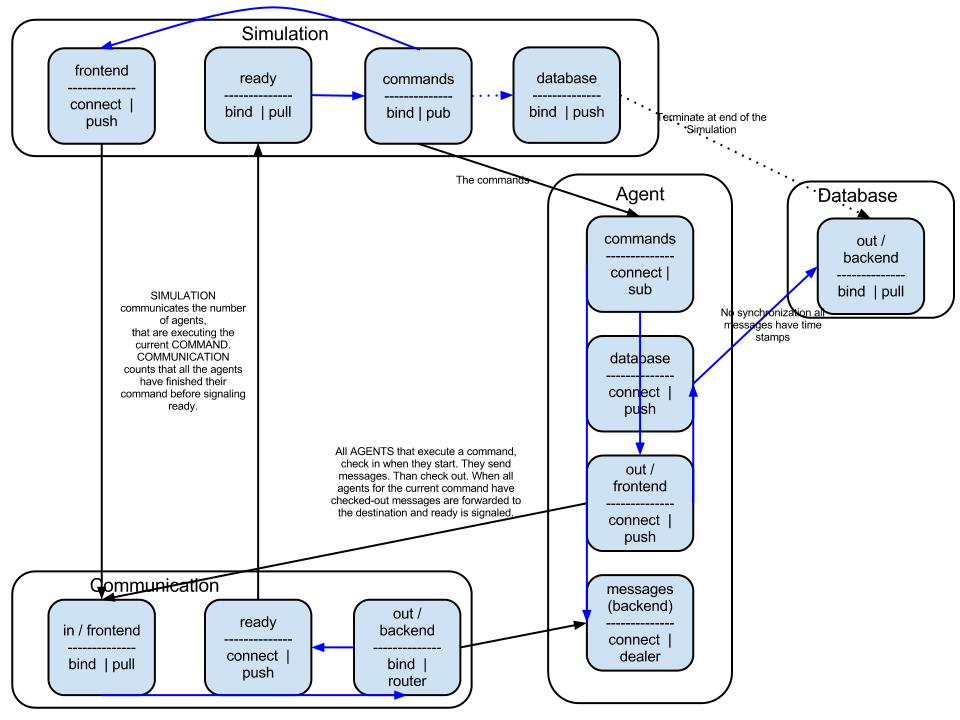
\includegraphics{messagemodel}}
\end{figure}

A simulation contains a number of rounds comprised of sub-rounds.
Every sub-round the following sequence of events occurs:

The simulation process manages the schedule, it sends the sub-round corresponding
to be executed to the agents and simultaneously sends the number of
agents that have received the order to execute this sub-round to the
communication agent. The agents then execute the sub-round, send
messages for other agents to the communication process; when
they are finished they signal this to the communication process. Once
all agents have signaled that they are finished the
communication process then distributes the messages to the
recipients. When the agents communicate that they have received
the messages, the communication process signals the completion
of a sub-round to simulation. The sub-round is concluded.

Agents also send messages to the logging process, messages to
the logging are not synchronized, but time stamped.

Message passing and synchronization are managed by a third
party library ZeroMQ \cite{hintjens2013zeromq}.
Every agent has four communication
sockets: one to receive commands, one to receive messages,
one to send data to the database and the last one to send
messages and signal the completion of the sub-round and reception
of messages. It is therefore imperative to have sockets that are
very small. What is more potentially millions of messages are
exchanged both in the execution of the program and as messages
representing the interaction between agents. Messaging speed
is therefore extremely important. ZeroMQ is a very small and
efficient transport protocol. \cite{Piel}. Further
it might become part of the Linux core.


\chapter{Download and Installation}
\label{installation:download-and-installation}\label{installation::doc}

\section{Installation of stable version Ubuntu}
\label{installation:installation-of-stable-version-ubuntu}\begin{enumerate}
\item {} 
Download stable version form:  \href{https://dl.dropboxusercontent.com/u/3655123/abce-0.3.tar.gz}{https://dl.dropboxusercontent.com/u/3655123/abce-0.3.tar.gz}

\item {} 
If pip is not installed in terminal:

\begin{Verbatim}[commandchars=\\\{\}]
sudo apt-get install python-pip, python-scipy, python-numpy
\end{Verbatim}

\item {} 
If R has not been installed automatically install it:

\begin{Verbatim}[commandchars=\\\{\}]
sudo apt-get install r-base
\end{Verbatim}

\item {} 
In terminal:

\begin{Verbatim}[commandchars=\\\{\}]
sudo pip install abce-0.3.1.tar.gz
\end{Verbatim}

\item {} 
Download templats and examples from: \href{https://dl.dropboxusercontent.com/u/3655123/abce\_templates-0.3.zip}{https://dl.dropboxusercontent.com/u/3655123/abce\_templates-0.3.zip}

\item {} 
unzip abce\_templates-0.3.zip

\end{enumerate}


\section{Installation of stable version Windows}
\label{installation:installation-of-stable-version-windows}\begin{enumerate}
\item {} 
Install Python2.7 (preferably 32bit)

\item {} 
Next, set the system’s PATH variable to include directories

\end{enumerate}
\begin{quote}

that include Python components and packages we’ll add later. To do this:
- Right-click Computer and select Properties.
- In the dialog box, select Advanced  System Settings.
- In the next dialog, select Environment Variables.
- In the User Variables section, edit the PATH statement to include this:

\begin{Verbatim}[commandchars=\\\{\}]
C:\PYGZbs{}Python27;C:\PYGZbs{}Python27\PYGZbs{}Lib\PYGZbs{}site-packages\PYGZbs{};C:\PYGZbs{}Python27\PYGZbs{}Scripts\PYGZbs{};
\end{Verbatim}
\end{quote}
\begin{enumerate}
\setcounter{enumi}{1}
\item {} 
Install Setuptools from \href{http://pypi.python.org/pypi/setuptools\#downloads}{http://pypi.python.org/pypi/setuptools\#downloads}

\item {} 
install pip:

\end{enumerate}
\begin{quote}

easy\_install pip
\end{quote}
\begin{enumerate}
\setcounter{enumi}{3}
\item {} 
Install R form www.cran.org

\item {} 
Download stable version form:  \href{https://dl.dropboxusercontent.com/u/3655123/abce-0.3.tar.gz}{https://dl.dropboxusercontent.com/u/3655123/abce-0.3.tar.gz}

\item {} 
install ABCE:

\end{enumerate}
\begin{quote}

pip install abce-0.3.1.tar.gz
\end{quote}

In case of problems reinstall python
\href{http://www.anthonydebarros.com/2011/10/15/setting-up-python-in-windows-7/}{http://www.anthonydebarros.com/2011/10/15/setting-up-python-in-windows-7/}
\begin{enumerate}
\setcounter{enumi}{6}
\item {} 
Download templats and examples from: \href{https://dl.dropboxusercontent.com/u/3655123/abce\_templates-0.3.zip}{https://dl.dropboxusercontent.com/u/3655123/abce\_templates-0.3.zip}

\item {} 
unzip abce\_templates-0.3.zip

\end{enumerate}


\section{Installation of development version}
\label{installation:installation-of-development-version}
The installation has two parts. Installing the necessary software packages. Retrieving ABCE with git or as a zip file.
\begin{quote}

Alternative 1 as a zip (EASY):
\begin{enumerate}
\item {} 
download the zip file from: \href{https://github.com/DavoudTaghawiNejad/abce}{https://github.com/DavoudTaghawiNejad/abce}

\item {} 
extract zip file

\end{enumerate}

Alternative 2 via git \footnote{
Git is a a version controll system. It is higly recommended to use it to make your development process more efficient and less error prone. \href{http://gitimmersion.com/}{http://gitimmersion.com/}
} in terminal (RECOMMENDED):

\begin{Verbatim}[commandchars=\\\{\}]
[register with git and automatize a secure connection with your computer]
sudo apt-get install git
mkdir abce
cd abce
git init
git pull git@github.com:DavoudTaghawiNejad/abce.git
\end{Verbatim}
\end{quote}

Optional for development you can install sphinx and sphinx-apidoc,
the system that created this documentation.  sphinx-apidoc
currently needs the newest version of sphinx.


\chapter{Walk through / Tutorial}
\label{Walk_through:walk-through-tutorial}\label{Walk_through::doc}
This tutorial is a step by step guide to create an agent-based model with ABCE.
In the following two text boxes, the two concepts that make ABCE special are
explained: The explicit modeling of tradeable goods and the optional concept
of a physically closed economy.
\setbox0\vbox{
\begin{minipage}{0.95\linewidth}
\textbf{Objects the other ontological object of agent-based models.}

\medskip

\begin{description}
\item[{Objects have a special stance in agent-based modeling:}] \leavevmode\begin{itemize}
\item {} 
objects can be recovered (resources)

\item {} 
exchanged (trade)

\item {} 
transformed (production)

\item {} 
consumed (transformed :-))

\item {} 
destroyed (not really) and time depreciated

\end{itemize}

ABCE, takes care of trade, production / transformation and consumption
of goods automatically. Good categories can also be made to perish or regrow.

\item[{Services or labor}] \leavevmode
We can model services and labor as goods that perish
and that are replenished every round. This would amount to a worker that can
sell one unit of labor every round, that disappears if not used.

\item[{Closed economy}] \leavevmode
When we impose that goods can only be transformed. The economy is physically
closed (the economy is stock and flow consistent). When the markets are in a
complete network our economy is complete. Think ``general'' in equilibrium
economics.

Caveats: If agents horde without taking their stock into account it's
like destruction.

\end{description}
\end{minipage}}
\begin{center}\setlength{\fboxsep}{5pt}\shadowbox{\box0}\end{center}

With this basic understanding you can now start writing your own model.

To create a model you basically have to follow three steps:
\begin{enumerate}
\item {} 
Specify endowments that replenish every round and goods / services that perish

\item {} 
Specify the order of actions

\item {} 
Write the agents with their actions

\end{enumerate}

There is of course a little bit of administrative work you have to do:
\begin{enumerate}
\item {} 
import agents in the model

\item {} 
specify parameters

\end{enumerate}


\section{Have a look on the \emph{abce/examples/} folder}
\label{Walk_through:have-a-look-on-the-abce-examples-folder}
It is instructive to look at a simple example, for example the 2x2 economy.
Then you can make a working copy of the template or a copy of an example.


\section{Make a working copy}
\label{Walk_through:make-a-working-copy}
copy abce/example to your\_model\_path:

\begin{Verbatim}[commandchars=\\\{\}]
cd your\_model\_path
cp path.to/abce/template/* .
\end{Verbatim}


\section{start.py}
\label{Walk_through:start-py}

\subsection{Overview}
\label{Walk_through:overview}
In start.py the simulation, thus the parameters, objects, agents and time line are
set up. Further it is declared, what is observed and written to the database. \footnote{
from \_\_future\_\_ import division, instructs python to handle division always as a
floating point division. Use this in all your python code. If you do not use this \code{3 / 2 = 1} instead
of \code{3 / 2 = 1.5} (floor division).
}

\begin{Verbatim}[commandchars=\\\{\}]
\PYG{k+kn}{from} \PYG{n+nn}{Firm} \PYG{k+kn}{import} \PYG{n}{Firm}
\PYG{k+kn}{from} \PYG{n+nn}{Household} \PYG{k+kn}{import} \PYG{n}{Household}
\end{Verbatim}

Here the Agent class Firm is imported from the file Firm.py. Likewise the Household class.

ABCE, reads the model parameter from a spreed sheet, every line is one simulation:

\begin{Verbatim}[commandchars=\\\{\}]
\PYG{k}{for} \PYG{n}{parameters} \PYG{o+ow}{in} \PYG{n}{simulation}\PYG{o}{.}\PYG{n}{read\PYGZus{}parameters}\PYG{p}{(}\PYG{l+s}{'}\PYG{l+s}{simulation\PYGZus{}parameters.csv}\PYG{l+s}{'}\PYG{p}{)}\PYG{p}{:}

   \PYG{o}{.}\PYG{o}{.}\PYG{o}{.}
\end{Verbatim}

With the parameters ABCE loops over the intended line, to create the simulation
and then runs the simulation. (after that it reads the next line an loops again).
The variable parameters contain all parameters from `simulation\_parameters.csv'.
See \emph{simulation\_parameters and agent\_parameters} for details.

To set up a new model, you create a class a that will comprise your model:

\begin{Verbatim}[commandchars=\\\{\}]
\PYG{n}{s} \PYG{o}{=} \PYG{n}{Simulation}\PYG{p}{(}\PYG{n}{parameters}\PYG{p}{)}

\PYG{o}{.}\PYG{o}{.}\PYG{o}{.}
\end{Verbatim}

After this the order of actions, agents and objects are added.

\begin{Verbatim}[commandchars=\\\{\}]
\PYG{n}{action\PYGZus{}list} \PYG{o}{=} \PYG{p}{[}
\PYG{p}{(}\PYG{l+s}{'}\PYG{l+s}{Household}\PYG{l+s}{'}\PYG{p}{,} \PYG{l+s}{'}\PYG{l+s}{offer\PYGZus{}capital}\PYG{l+s}{'}\PYG{p}{)}\PYG{p}{,}

\PYG{o}{.}\PYG{o}{.}\PYG{o}{.}

\PYG{p}{(}\PYG{l+s}{'}\PYG{l+s}{Household}\PYG{l+s}{'}\PYG{p}{,} \PYG{l+s}{'}\PYG{l+s}{consumption}\PYG{l+s}{'}\PYG{p}{)}
\PYG{p}{]}
\PYG{n}{s}\PYG{o}{.}\PYG{n}{add\PYGZus{}action\PYGZus{}list}\PYG{p}{(}\PYG{n}{action\PYGZus{}list}\PYG{p}{)}
\end{Verbatim}

This establishes the order of the simulation. It can also be read from file {\hyperref[simulation:abce.Simulation.add_action_list_from_file]{\code{abce.Simulation.add\_action\_list\_from\_file()}}}

In order to add an agent which was imported before we simply build these agents:

\begin{Verbatim}[commandchars=\\\{\}]
\PYG{n}{s}\PYG{o}{.}\PYG{n}{build\PYGZus{}agents}\PYG{p}{(}\PYG{n}{Firm}\PYG{p}{,} \PYG{l+s}{'}\PYG{l+s}{number\PYGZus{}of\PYGZus{}firms}\PYG{l+s}{'}\PYG{p}{)}
\PYG{n}{s}\PYG{o}{.}\PYG{n}{build\PYGZus{}agents}\PYG{p}{(}\PYG{n}{Household}\PYG{p}{,} \PYG{l+m+mi}{10}\PYG{p}{)}
\end{Verbatim}

The number of firms to be built is read from the column in simulation\_parameters.csv called number\_of\_firms.
The number of households on the other side is fixed at 10.

Or you can create panel data for a group of agents:

\begin{Verbatim}[commandchars=\\\{\}]
\PYG{n}{s}\PYG{o}{.}\PYG{n}{panel\PYGZus{}db}\PYG{p}{(}\PYG{l+s}{'}\PYG{l+s}{Firm}\PYG{l+s}{'}\PYG{p}{,} \PYG{n}{command}\PYG{o}{=}\PYG{l+s}{'}\PYG{l+s}{after\PYGZus{}sales\PYGZus{}before\PYGZus{}consumption}\PYG{l+s}{'}\PYG{p}{)}
\PYG{n}{s}\PYG{o}{.}\PYG{n}{panel\PYGZus{}db}\PYG{p}{(}\PYG{l+s}{'}\PYG{l+s}{Household}\PYG{l+s}{'}\PYG{p}{)}  \PYG{c}{\PYGZsh{} at the beginning}
\PYG{o}{.}\PYG{o}{.}\PYG{o}{.}

\PYG{n}{s}\PYG{o}{.}\PYG{n}{run}\PYG{p}{(}\PYG{p}{)}
\end{Verbatim}


\subsection{The order of actions: The order of actions within a round}
\label{Walk_through:the-order-of-actions-the-order-of-actions-within-a-round}
Every agents-based model is characterized by the order of which the actions are executed. In ABCE, there are rounds, every round is composed of sub-rounds, in which all agents, a group of agents or a single agent, act in parallel. In the
code below you see a typical sub-round.

You have to declare an action\_list, that is made of tuples telling ABCE which
agent or agent group, should execute which method:

\begin{Verbatim}[commandchars=\\\{\}]
\PYG{n}{action\PYGZus{}list} \PYG{o}{=} \PYG{p}{[}
\PYG{n}{repeat}\PYG{p}{(}\PYG{p}{[}
    \PYG{p}{(}\PYG{l+s}{'}\PYG{l+s}{Household}\PYG{l+s}{'}\PYG{p}{,} \PYG{l+s}{'}\PYG{l+s}{offer\PYGZus{}capital}\PYG{l+s}{'}\PYG{p}{)}\PYG{p}{,}
    \PYG{p}{(}\PYG{l+s}{'}\PYG{l+s}{Firm}\PYG{l+s}{'}\PYG{p}{,} \PYG{l+s}{'}\PYG{l+s}{buy\PYGZus{}capital}\PYG{l+s}{'}\PYG{p}{)}\PYG{p}{,}
\PYG{p}{]}\PYG{p}{,}
\PYG{n}{repetitions}\PYG{o}{=}\PYG{l+m+mi}{10}\PYG{p}{)}\PYG{p}{,}
\PYG{p}{(}\PYG{l+s}{'}\PYG{l+s}{Household}\PYG{l+s}{'}\PYG{p}{,} \PYG{l+s}{'}\PYG{l+s}{search\PYGZus{}work}\PYG{l+s}{'}\PYG{p}{)}\PYG{p}{,}
\PYG{p}{(}\PYG{l+s}{'}\PYG{l+s}{Firm}\PYG{l+s}{'}\PYG{p}{,} \PYG{l+s}{'}\PYG{l+s}{hire\PYGZus{}labor}\PYG{l+s}{'}\PYG{p}{)}\PYG{p}{,}
\PYG{p}{(}\PYG{l+s}{'}\PYG{l+s}{Firm}\PYG{l+s}{'}\PYG{p}{,} \PYG{l+s}{'}\PYG{l+s}{production}\PYG{l+s}{'}\PYG{p}{)}\PYG{p}{,}
\PYG{l+s}{'}\PYG{l+s}{after\PYGZus{}sales\PYGZus{}before\PYGZus{}consumption}\PYG{l+s}{'}\PYG{p}{,}
\PYG{p}{(}\PYG{l+s}{'}\PYG{l+s}{Household}\PYG{l+s}{'}\PYG{p}{,} \PYG{l+s}{'}\PYG{l+s}{consumption}\PYG{l+s}{'}\PYG{p}{)}
\PYG{p}{]}
\PYG{n}{s}\PYG{o}{.}\PYG{n}{add\PYGZus{}action\PYGZus{}list}\PYG{p}{(}\PYG{n}{action\PYGZus{}list}\PYG{p}{)}
\end{Verbatim}

The first tuple for example tells all Household agents to execute the method ``offer\_capital''.
The `after\_sales\_before\_consumption' is a database command. see \code{abce.panel\_db()}.

The repeat function allows repeating actions within the brackets a determinate amount of times.

Interactions happen between sub-rounds. An agent, sends a message in one round.
The receiving agent, receives the message the following sub-round.  A trade is
finished in three rounds: (1) an agent sends an offer the good is blocked, so it
can not be sold twice (2) the other agent accepts or rejects it. (3) If
accepted, the good is automatically delivered. If the trade was rejected: the
blocked good is unblocked.


\subsection{The goods}
\label{Walk_through:the-goods}
A normal good can be traded and used for production or consumption.
The only thing you have to do is create the amount of goods for every agent with
{\hyperref[Agent_class:abce.Agent.create]{\code{abce.Agent.create()}}} in the agent's \_\_init\_\_ method.

If an agent receives an endowment every round this can be automatically handled,
with {\hyperref[simulation:abce.Simulation.declare_round_endowment]{\code{abce.Simulation.declare\_round\_endowment()}}}.
For example the following command gives, at the beginning of every round,
to whom who possess one unit of `field' 100 units of `corn':

\begin{Verbatim}[commandchars=\\\{\}]
\PYG{n}{s}\PYG{o}{.}\PYG{n}{declare\PYGZus{}round\PYGZus{}endowment}\PYG{p}{(}\PYG{l+s}{'}\PYG{l+s}{field}\PYG{l+s}{'}\PYG{p}{,} \PYG{l+m+mi}{100}\PYG{p}{,} \PYG{l+s}{'}\PYG{l+s}{corn}\PYG{l+s}{'}\PYG{p}{)}
\end{Verbatim}

You can also declare goods that last only one round and then automatically perish.
{\hyperref[simulation:abce.Simulation.declare_perishable]{\code{abce.Simulation.declare\_perishable()}}}

\begin{Verbatim}[commandchars=\\\{\}]
\PYG{n}{s}\PYG{o}{.}\PYG{n}{declare\PYGZus{}perishable}\PYG{p}{(}\PYG{l+s}{'}\PYG{l+s}{corn}\PYG{l+s}{'}\PYG{p}{)}
\end{Verbatim}

This example declares `corn' perishable and every round the agent gets 100 units of
of `corn' for every unit of field he possesses. If the corn is not consumed, it
automatically disappears at the end of the round.

One important remark, for a logically consistent \textbf{macro-model} it is best to
not create any goods during the simulation, but only in
\code{abce.Agent.\_\_init\_\_()}. During the simulation the only new goods
should be created by declare\_round\_endowment. In this way the economy is physically
closed. An exception is, of course, money.


\section{The agents}
\label{Walk_through:the-agents}
Agents are modeled in a separate file. In the template directory, you will find
three agents: agent.py, firm.py and household.py.

At the beginning of each agent you will again find:

\begin{Verbatim}[commandchars=\\\{\}]
\PYG{k+kn}{from} \PYG{n+nn}{\PYGZus{}\PYGZus{}future\PYGZus{}\PYGZus{}} \PYG{k+kn}{import} \PYG{n}{division}
\end{Verbatim}

An agent has to import the {\hyperref[simulation:module-abce]{\code{abce}}} module and some helpers:

\begin{Verbatim}[commandchars=\\\{\}]
\PYG{k+kn}{import} \PYG{n+nn}{abce}
\PYG{k+kn}{from} \PYG{n+nn}{abcetools} \PYG{k+kn}{import} \PYG{n}{is\PYGZus{}zero}\PYG{p}{,} \PYG{n}{is\PYGZus{}positive}\PYG{p}{,} \PYG{n}{is\PYGZus{}negative}\PYG{p}{,} \PYG{n}{NotEnoughGoods}
\end{Verbatim}

This imports the base classes: abce, Household and Firm.

An agent is a class and must at least inherit {\hyperref[Agent_class:abce.Agent]{\code{abce.Agent}}}.
{\hyperref[Trade:abce.Trade]{\code{abce.Trade}}} - {\hyperref[Messaging:messaging.Messaging]{\code{messaging.Messaging}}} and {\hyperref[Database:database.Database]{\code{database.Database}}}
are automatically inherited:

\begin{Verbatim}[commandchars=\\\{\}]
class Agent(abce.Agent):
\end{Verbatim}

To create an agent that can also consume:

\begin{Verbatim}[commandchars=\\\{\}]
class Household(abce.Agent, abce.Household):
\end{Verbatim}

You see our Household agent inherits from {\hyperref[Agent_class:abce.Agent]{\code{abce.Agent}}}, which is compulsory and {\hyperref[Household:abce.Household]{\code{abce.Household}}}.
Household on the other hand are a set of methods that are unique for Household agents.
(there is also a Firm class)


\subsection{The \_\_init\_\_ method}
\label{Walk_through:the-init-method}
\begin{Verbatim}[commandchars=\\\{\}]
\PYG{k}{def} \PYG{n+nf}{\PYGZus{}\PYGZus{}init\PYGZus{}\PYGZus{}}\PYG{p}{(}\PYG{n+nb+bp}{self}\PYG{p}{,} \PYG{n}{simulation\PYGZus{}parameters}\PYG{p}{,} \PYG{n}{agent\PYGZus{}parameters}\PYG{p}{,} \PYG{n}{\PYGZus{}pass\PYGZus{}to\PYGZus{}engine}\PYG{p}{)}\PYG{p}{:}
    \PYG{n}{abce}\PYG{o}{.}\PYG{n}{\PYGZus{}\PYGZus{}init\PYGZus{}\PYGZus{}}\PYG{p}{(}\PYG{n+nb+bp}{self}\PYG{p}{,} \PYG{o}{*}\PYG{n}{\PYGZus{}pass\PYGZus{}to\PYGZus{}engine}\PYG{p}{)}
    \PYG{n+nb+bp}{self}\PYG{o}{.}\PYG{n}{create}\PYG{p}{(}\PYG{l+s}{'}\PYG{l+s}{labor\PYGZus{}endowment}\PYG{l+s}{'}\PYG{p}{,} \PYG{l+m+mi}{1}\PYG{p}{)}
    \PYG{n+nb+bp}{self}\PYG{o}{.}\PYG{n}{create}\PYG{p}{(}\PYG{l+s}{'}\PYG{l+s}{capital\PYGZus{}endowment}\PYG{l+s}{'}\PYG{p}{,} \PYG{l+m+mi}{1}\PYG{p}{)}
    \PYG{n+nb+bp}{self}\PYG{o}{.}\PYG{n}{set\PYGZus{}cobb\PYGZus{}douglas\PYGZus{}utility\PYGZus{}function}\PYG{p}{(}\PYG{p}{\PYGZob{}}\PYG{l+s}{"}\PYG{l+s}{MLK}\PYG{l+s}{"}\PYG{p}{:} \PYG{l+m+mf}{0.300}\PYG{p}{,} \PYG{l+s}{"}\PYG{l+s}{BRD}\PYG{l+s}{"}\PYG{p}{:} \PYG{l+m+mf}{0.700}\PYG{p}{\PYGZcb{}}\PYG{p}{)}
    \PYG{n+nb+bp}{self}\PYG{o}{.}\PYG{n}{prices} \PYG{o}{=} \PYG{p}{\PYGZob{}}\PYG{p}{\PYGZcb{}}
    \PYG{n+nb+bp}{self}\PYG{o}{.}\PYG{n}{prices}\PYG{p}{[}\PYG{l+s}{'}\PYG{l+s}{labor}\PYG{l+s}{'}\PYG{p}{]} \PYG{o}{=} \PYG{l+m+mi}{1}
    \PYG{n+nb+bp}{self}\PYG{o}{.}\PYG{n}{number\PYGZus{}of\PYGZus{}firms} \PYG{o}{=} \PYG{n}{simulation\PYGZus{}parameters}\PYG{p}{[}\PYG{l+s}{'}\PYG{l+s}{number\PYGZus{}of\PYGZus{}firms}\PYG{l+s}{'}\PYG{p}{]}
    \PYG{n+nb+bp}{self}\PYG{o}{.}\PYG{n}{renter} \PYG{o}{=} \PYG{n}{random}\PYG{o}{.}\PYG{n}{randint}\PYG{p}{(}\PYG{l+m+mi}{0}\PYG{p}{,} \PYG{l+m+mi}{100}\PYG{p}{)}
    \PYG{n+nb+bp}{self}\PYG{o}{.}\PYG{n}{last\PYGZus{}utility} \PYG{o}{=} \PYG{n+nb+bp}{None}
\end{Verbatim}

The \_\_init\_\_ method is the method that is called when the agents are created (by
the {\hyperref[simulation:abce.Simulation.build_agents]{\code{abce.Simulation.build\_agents()}}} or {\hyperref[simulation:abce.Simulation.build_agents_from_file]{\code{abce.Simulation.build\_agents\_from\_file()}}} method.)
In this method agents can access the simulation\_parameters from the `simulation\_parameters.csv'.

If the agents are built using {\hyperref[simulation:abce.Simulation.build_agents_from_file]{\code{abce.Simulation.build\_agents\_from\_file()}}}. The agents
can access the parameters in their row, in `agents\_parameters.csv', by
agent\_parameters in the \_\_init\_\_ function.

Line 2 is compulsory to pass the parameters to the abce.

With self.create the agent creates the good `labor\_endowment'. Any
good can be created. Generally speaking. The \_\_init\_\_ method is the only place
where it is consistent to create a good. (except for money, if you simulate a naive
central bank).

This agent class inherited {\hyperref[Household:abce.Household.set_cobb_douglas_utility_function]{\code{abce.Household.set\_cobb\_douglas\_utility\_function()}}}
from {\hyperref[Household:abce.Household]{\code{abce.Household}}}. With
{\hyperref[Household:abce.Household.set_cobb_douglas_utility_function]{\code{abce.Household.set\_cobb\_douglas\_utility\_function()}}} you can create a
cobb-douglas function. Other functional forms are also available.

self.prices is a dictionary, created by the modeler, that saves prices for
specific goods. Here the price for labor is set to 1.

In order to let the agent remember a simulation\_parameter it has to be saved in the self
domain the agent.  \footnote{
(self.number\_of\_firms = simulation\_parameters{[}'number\_of\_firms'{]})
}

There is a random number assigned to self.renter and self.last\_utility is initialized
with None. It is often necessary to initialize variable in the \_\_init\_\_ method to
avoid errors in the first round.


\subsection{The action methods and a consuming Household}
\label{Walk_through:the-action-methods-and-a-consuming-household}
All the other methods of the agent are executed when the corresponding sub-round is
called from the Simulation set up in start.py.  \footnote{
With the exception of methods, whose names start with a `\_' underscore.underscoring methods that the agent uses only internally can speed up your code.
}

For example when in the action list \emph{(`household', `eat')} is called the eat method
is executed of each household agent is executed:

\begin{Verbatim}[commandchars=\\\{\}]
class Agent(abce.Agent, abce.Household)
    def \_\_init\_\_(self):
        self.set\_cobb\_douglas\_utility\_function(\PYGZob{}'cookies': 0.9', 'bread': 0.1\PYGZcb{})
        self.create('cookies', 1)
        self.create('bread', 5)

...
def eat(self):
    utility = self.consume\_everything()
    self.log('utility', \PYGZob{}'a': utility\PYGZcb{})
\end{Verbatim}

In the above example we see how a utility function is declared and how the
agent consumes. The utility is logged and can be retrieved see
{\hyperref[simulation_results:rsr]{\emph{retrieval of the simulation results}}}


\subsection{Firms and Production functions}
\label{Walk_through:firms-and-production-functions}
Firms do two things they produce (transform) and trade. The following
code shows you how to declare a technology and produce bread from labor and
yeast.

\begin{Verbatim}[commandchars=\\\{\}]
class Agent(abce.Agent, abce.Household):
def init(self):
   set\_cobb\_douglas('BRD', 1.890, \PYGZob{}"yeast": 0.333, "LAB": 0.667\PYGZcb{})
    ..
def production(self):
    self.produce\_use\_everything()
\end{Verbatim}

More details in {\hyperref[Firm:abce.Firm]{\code{abce.Firm}}}. {\hyperref[FirmMultiTechnologies:abce.FirmMultiTechnologies]{\code{abce.FirmMultiTechnologies}}} offers
a more advanced interface for firms with complicated technologies.


\subsection{Trade}
\label{Walk_through:trade}
ABCE handles trade fully automatically. That means, that goods are automatically
exchanged, double selling of a good is avoided by subtracting a good from
the possessions when it is offered
for sale. The modeler has only to decide when the agent offers a
trade and sets the criteria to accept the trade:

\begin{Verbatim}[commandchars=\\\{\}]
\PYG{c}{\PYGZsh{} Agent 1}
\PYG{k}{def} \PYG{n+nf}{selling}\PYG{p}{(}\PYG{n+nb+bp}{self}\PYG{p}{)}\PYG{p}{:}
    \PYG{n}{offerid} \PYG{o}{=} \PYG{n+nb+bp}{self}\PYG{o}{.}\PYG{n}{sell}\PYG{p}{(}\PYG{n}{buyer}\PYG{p}{,} \PYG{l+s}{'}\PYG{l+s}{BRD}\PYG{l+s}{'}\PYG{p}{,} \PYG{l+m+mi}{1}\PYG{p}{,} \PYG{l+m+mf}{2.5}\PYG{p}{)}
    \PYG{n+nb+bp}{self}\PYG{o}{.}\PYG{n}{checkorders}\PYG{o}{.}\PYG{n}{append}\PYG{p}{(}\PYG{n}{offerid}\PYG{p}{)}

\PYG{c}{\PYGZsh{} Agent 2}
\PYG{k}{def} \PYG{n+nf}{buying}\PYG{p}{(}\PYG{n+nb+bp}{self}\PYG{p}{)}\PYG{p}{:}
    \PYG{n}{offers} \PYG{o}{=} \PYG{n+nb+bp}{self}\PYG{o}{.}\PYG{n}{get\PYGZus{}offers}\PYG{p}{(}\PYG{l+s}{'}\PYG{l+s}{cookies}\PYG{l+s}{'}\PYG{p}{)}
    \PYG{k}{for} \PYG{n}{offer} \PYG{o+ow}{in} \PYG{n}{offers}\PYG{p}{:}
       \PYG{k}{try}\PYG{p}{:}
          \PYG{n+nb+bp}{self}\PYG{o}{.}\PYG{n}{accept}\PYG{p}{(}\PYG{n}{offer}\PYG{p}{)}
       \PYG{k}{except} \PYG{n}{NotEnoughGoods}\PYG{p}{:}
          \PYG{n+nb+bp}{self}\PYG{o}{.}\PYG{n}{reject}\PYG{p}{(}\PYG{n}{offer}\PYG{p}{)}
\end{Verbatim}

You can find a detailed explanation how trade works in {\hyperref[Trade:abce.Trade]{\code{abce.Trade}}}


\subsection{Data production}
\label{Walk_through:data-production}
There are three different ways of observing your agents:


\subsubsection{Trade Logging}
\label{Walk_through:trade-logging}
ABCE by default logs all trade and creates a SAM or IO matrix.


\subsubsection{Manual in agent logging}
\label{Walk_through:manual-in-agent-logging}
An agent can log a variable, {\hyperref[Agent_class:abce.Agent.possessions]{\code{abce.Agent.possessions()}}}, {\hyperref[Agent_class:abce.Agent.possessions_all]{\code{abce.Agent.possessions\_all()}}}
and most other methods such as {\hyperref[Firm:abce.Firm.produce]{\code{abce.Firm.produce()}}} with \code{abce.Agent.log()} or a
change in a variable with {\hyperref[Database:database.Database.log_change]{\code{log\_change()}}}:

\begin{Verbatim}[commandchars=\\\{\}]
self.log('possessions', self.possesions\_all())
self.log('custom', \PYGZob{}'price\_setting': 5: 'production\_value': 12\PYGZcb{})
prod = self.production\_use\_everything()
self.log('current\_production', prod)
\end{Verbatim}


\subsubsection{Panel Data}
\label{Walk_through:panel-data}
{\hyperref[simulation:abce.Simulation.panel_data]{\code{panel\_data()}}} creates panel data for all agents in a specific
agent group at a specific point in every round. It is set in start.py:

\begin{Verbatim}[commandchars=\\\{\}]
s.panel\_data(’Household’, command=’aftersalesbeforeconsumption’)
\end{Verbatim}

The command has to be inserted in the action\_list.


\subsubsection{Retrieving the logged data}
\label{Walk_through:retrieving-the-logged-data}
the results are stored in a subfolder of the ./results/ folder.

The tables are stored as `.csv' files which can be opened with excel and
libreoffice.
Further you can import the files with R:
\begin{enumerate}
\item {} 
change to the subfolder of ./results/ that contains your simulation
results

\item {} 
start R

\item {} 
\emph{load(`database.R')}

\end{enumerate}


\chapter{Examples}
\label{examples::doc}\label{examples:examples}
ABCE comes with two example projects `one\_household\_one\_firm', describes
a one sector economy with one representative firm and household, `2sectors',
describes a two sector economy with one representative household


\section{One sector model}
\label{examples:one-sector-model}
One household one firm is a minimalistic example of a `macro-economy'.
It is `macro' in the sense that the complete circular flow of the economy is
represented. Every round the following sub-rounds are executed:
\begin{quote}
\begin{description}
\item[{household:}] \leavevmode
sell\_labor

\item[{firm:}] \leavevmode
buy\_labor

\item[{firm:}] \leavevmode
production

\item[{firm:}] \leavevmode
sell\_goods

\item[{household:}] \leavevmode
buy\_goods

\item[{household:}] \leavevmode
consumption

\end{description}
\end{quote}

After the firms' production and the acquisition of goods by the household
a statistical panel of the firms' and the households' possessions, respectively,
is written to the database.

The economy has two goods a representative `GOOD' good and `labor' as
well as money. `labor', which is a service that is represented as a good that
perishes every round when it is not used. Further the endowment is
of the labor good that is replenished every round for every agent that
has an `adult'. `Adults' are handled like possessions of the household agent.

The household has a degenerate Cobb-Douglas utility function and the firm
has a degenerate Cobb-Douglas production function:

\begin{Verbatim}[commandchars=\\\{\}]
\PYG{n}{utility} \PYG{o}{=} \PYG{n}{GOOD} \PYG{o}{\PYGZca{}} \PYG{l+m+mi}{1}

\PYG{n}{GOOD} \PYG{o}{=} \PYG{n}{labor} \PYG{o}{\PYGZca{}} \PYG{l+m+mi}{1}
\end{Verbatim}

The firms own an initial amount of money of 1 and the household
has one adult, which supplies one unit of (perishable) labor every
round.

First the household sells his unit of labor. The firm buys this unit
and uses all available labor for production. The complete production
is offered to the household, which in turn buys everything it can afford.
The good is consumed and the resulting utility logged to the database.


\section{Two sector model}
\label{examples:two-sector-model}
The two sector model is similar to the one sector model. It has two
firms and showcases ABCE's ability to control the creation of agents
from an excel sheet.

There are two firms. One firm manufactures an intermediary good. The
other firm produces the final good. Both firms are implemented with
the same good. The type a firm develops is based on the excel sheet.

The two respective firms production functions are:

\begin{Verbatim}[commandchars=\\\{\}]
\PYG{n}{intermediate\PYGZus{}good} \PYG{o}{=} \PYG{n}{labor} \PYG{o}{\PYGZca{}} \PYG{l+m+mi}{1}

\PYG{n}{consumption\PYGZus{}good} \PYG{o}{=} \PYG{n}{intermediate\PYGZus{}good} \PYG{o}{\PYGZca{}} \PYG{l+m+mi}{1} \PYG{o}{*} \PYG{n}{labor} \PYG{o}{\PYGZca{}} \PYG{l+m+mi}{1}
\end{Verbatim}

The only difference is that, when firms sell their products the
intermedate good firm sells to the final good firm and the final
good firm, in the same sub-round sells to the household.

In start.py we can see that the firms that are build are build
from an excel sheet:
\begin{quote}

w.build\_agents\_from\_file(Firm, parameters\_file='agents\_parameters.csv')
w.build\_agents\_from\_file(Household)
\end{quote}

And here the excel sheet:
\begin{quote}

agent\_class number  sector
firm        1   intermediate\_good
firm        1   consumption\_good
household   1   0
household   1   1
\end{quote}

The advantage of this is that the parameters can be used in the agent.
The line \emph{self.sector = agent\_parameters{[}'sector'{]}} reads the sector
column and assigns it to the self.sector variable. The file simulation
parameters is read - line by line - into the variable simulation\_parameters.
It can be used in start.py and in the agents with
simulation\_parameters{[}'columnlabel'{]}.


\chapter{unit testing}
\label{unit_testing:unit-testing}\label{unit_testing::doc}
One of the major problem of doing science with simulations is that
results found could be a mere result of a mistake in the software
implementation. This problem is even stronger when emergent phenomena
are expected. The first hedge against this problem is of course
carefully checking the code. ABCE and Pythons brevity  and readability
are certainly helping this. However structured testing procedures
create more robust software.

Currently all trade and exchange related as well as endowment and
data logging facilities are unit tested. It is planned to extend
unit testing to production and consumption, so that by version 0.4
all functions of the agents will be fully unit tested.

The modeler can run the unit testing facilities on his own system and therefore
assert that on his own system the code runs correctly.

Unit testing is the testing of the testable part of a the software code.
\cite{Xie2007}. As in ABCE the most crucial functions are
the exchange of goods or information, the smallest testable unit is often
a combination of two actions \cite{Aniche}. For example making an offer and then by
a second agent accepting or rejecting it. The interaction and concurrent
nature of ABCE simulation make it unpractical to use the standard unit
testing procedures of Python.

\cite{Ellims2006} argue that unit-testing is economical. In
the analysis of three projects they find that unit-testing finds errors
in the code and argue that its cost is often exaggerated. We can
therefore conclude that unit-testing is necessary and a cost efficient
way of ensuring the correctness of the results of the simulation. For
the modeler this is an additional incentive to use ABCE, if he
implemented the simulation as a stand alone program he would either have
to forgo the testing of the agent's functions or write his own unit-testing
facilities.


\chapter{Agents}
\label{Agent_class:module-agent}\label{Agent_class:agents}\label{Agent_class::doc}\index{agent (module)}
The \code{abce.agent.Agent} class is the basic class for creating your agents. It automatically handles the
possession of goods of an agent. In order to produce/transforme goods you also need to subclass
the \code{abceagent.Firm} \footnote{
or \code{abce.agent.FirmMultiTechnologies} for simulations with complex technologies.
} or to create a consumer the \code{abce.agent.Household}.

For detailed documentation on:
\begin{description}
\item[{Trading:}] \leavevmode
see \code{abce.agent.Trade}

\item[{Logging and data creation:}] \leavevmode
see \code{abce.agent.Database} and {\hyperref[simulation_results::doc]{\emph{Retrieval of the simulation results}}}

\item[{Messaging between agents:}] \leavevmode
see \code{abce.agent.Messaging}.

\end{description}
\index{NotEnoughGoods}

\begin{fulllineitems}
\phantomsection\label{Agent_class:abce.tools.NotEnoughGoods}\pysiglinewithargsret{\strong{exception }\code{abce.tools.}\bfcode{NotEnoughGoods}}{\emph{\_agent\_name}, \emph{good}, \emph{amount\_missing}}{}
Methods raise this exception when the agent has less goods than needed

These functions (self.produce, self.offer, self.sell, self.buy)
should be encapsulated by a try except block:

\begin{Verbatim}[commandchars=\\\{\}]
\PYG{k}{try}\PYG{p}{:}
   \PYG{n+nb+bp}{self}\PYG{o}{.}\PYG{n}{produce}\PYG{p}{(}\PYG{o}{.}\PYG{o}{.}\PYG{o}{.}\PYG{p}{)}
\PYG{k}{except} \PYG{n}{NotEnoughGoods}\PYG{p}{:}
   \PYG{n}{alternative\PYGZus{}statements}\PYG{p}{(}\PYG{p}{)}
\end{Verbatim}

\end{fulllineitems}

\index{Agent (class in abce)}

\begin{fulllineitems}
\phantomsection\label{Agent_class:abce.Agent}\pysiglinewithargsret{\strong{class }\code{abce.}\bfcode{Agent}}{\emph{idn}, \emph{group}, \emph{\_addresses}, \emph{trade\_logging}}{}
Bases: \code{abce.database.Database}, \code{abce.logger.Logger}, \code{abce.trade.Trade}, \code{abce.messaging.Messaging}, \code{multiprocessing.process.Process}

Every agent has to inherit this class. It connects the agent to the simulation
and to other agent. The \code{abceagent.Trade}, \code{abceagent.Database} and
\code{abceagent.Messaging} classes are included. You can enhance an agent, by also
inheriting from \code{abceagent.Firm}.:class:\emph{abceagent.FirmMultiTechnologies}
or \code{abceagent.Household}.

For example:

\begin{Verbatim}[commandchars=\\\{\}]
class Household(abceagent.Agent, abceagent.Household):
    def \_\_init\_\_(self, simulation\_parameters, agent\_parameters, \_pass\_to\_engine):
    abceagent.Agent.\_\_init\_\_(self, *\_pass\_to\_engine)
\end{Verbatim}
\index{aesof\_eval() (abce.Agent method)}

\begin{fulllineitems}
\phantomsection\label{Agent_class:abce.Agent.aesof_eval}\pysiglinewithargsret{\bfcode{aesof\_eval}}{\emph{column\_name}}{}
evaluates an expression' in your excel file. see instruction of pythons eval commmand

\end{fulllineitems}

\index{aesof\_exec() (abce.Agent method)}

\begin{fulllineitems}
\phantomsection\label{Agent_class:abce.Agent.aesof_exec}\pysiglinewithargsret{\bfcode{aesof\_exec}}{\emph{column\_name}}{}
executes a command in your excel file. see instruction of pythons exec commmand

\end{fulllineitems}

\index{create() (abce.Agent method)}

\begin{fulllineitems}
\phantomsection\label{Agent_class:abce.Agent.create}\pysiglinewithargsret{\bfcode{create}}{\emph{good}, \emph{quantity}}{}
creates quantity of the good out of nothing

Use create with care, as long as you use it only for labor and
natural resources your model is macroeconomally complete.
\begin{description}
\item[{Args:}] \leavevmode
`good': is the name of the good
quantity: number

\end{description}

\end{fulllineitems}

\index{destroy() (abce.Agent method)}

\begin{fulllineitems}
\phantomsection\label{Agent_class:abce.Agent.destroy}\pysiglinewithargsret{\bfcode{destroy}}{\emph{good}, \emph{quantity}}{}
destroys quantity of the good,

Args:

\begin{Verbatim}[commandchars=\\\{\}]
'good': is the name of the good
quantity: number
\end{Verbatim}

Raises:

\begin{Verbatim}[commandchars=\\\{\}]
NotEnoughGoods: when goods are insufficient
\end{Verbatim}

\end{fulllineitems}

\index{destroy\_all() (abce.Agent method)}

\begin{fulllineitems}
\phantomsection\label{Agent_class:abce.Agent.destroy_all}\pysiglinewithargsret{\bfcode{destroy\_all}}{\emph{good}}{}
destroys all of the good, returns how much

Args:

\begin{Verbatim}[commandchars=\\\{\}]
'good': is the name of the good
\end{Verbatim}

\end{fulllineitems}

\index{possession() (abce.Agent method)}

\begin{fulllineitems}
\phantomsection\label{Agent_class:abce.Agent.possession}\pysiglinewithargsret{\bfcode{possession}}{\emph{good}}{}
returns how much of good an agent possesses.
\begin{description}
\item[{Returns:}] \leavevmode
A number.

\end{description}

possession does not return a dictionary for self.log(...), you can use self.possessions({[}...{]})
(plural) with self.log.

Example:
\begin{quote}
\begin{description}
\item[{if self.possession(`money') \textless{} 1:}] \leavevmode
self.financial\_crisis = True

\item[{if not(is\_positive(self.possession(`money')):}] \leavevmode
self.bancrupcy = True

\end{description}
\end{quote}

\end{fulllineitems}

\index{possessions() (abce.Agent method)}

\begin{fulllineitems}
\phantomsection\label{Agent_class:abce.Agent.possessions}\pysiglinewithargsret{\bfcode{possessions}}{\emph{list\_of\_goods}}{}
returns a dictionary of goods and the corresponding amount an agent owns
\begin{description}
\item[{Argument:}] \leavevmode
A list with good names. Can be a list with a single element.

\item[{Returns:}] \leavevmode
A dictionary, that can be used with self.log(..)

\end{description}

Examples:

\begin{Verbatim}[commandchars=\\\{\}]
self.log('buget', self.possesions(['money']))

self.log('goods', self.possesions(['gold', 'wood', 'grass']))

have = self.possessions(['gold', 'wood', 'grass']))
for good in have:
    if have[good] \textgreater{} 5:
        rich = True
\end{Verbatim}

\end{fulllineitems}

\index{possessions\_all() (abce.Agent method)}

\begin{fulllineitems}
\phantomsection\label{Agent_class:abce.Agent.possessions_all}\pysiglinewithargsret{\bfcode{possessions\_all}}{}{}
returns all possessions

\end{fulllineitems}

\index{possessions\_filter() (abce.Agent method)}

\begin{fulllineitems}
\phantomsection\label{Agent_class:abce.Agent.possessions_filter}\pysiglinewithargsret{\bfcode{possessions\_filter}}{\emph{goods=None}, \emph{but=None}, \emph{match=None}, \emph{beginswith=None}, \emph{endswith=None}}{}
returns a subset of the goods an agent owns, all arguments
can be combined.
\begin{description}
\item[{Args:}] \leavevmode\begin{description}
\item[{goods (list, optional):}] \leavevmode
a list of goods to return

\item[{but(list, optional):}] \leavevmode
all goods but the list of goods here.

\item[{match(string, optional TODO):}] \leavevmode
goods that match pattern

\item[{beginswith(string, optional):}] \leavevmode
all goods that begin with string

\item[{endswith(string, optional)}] \leavevmode
all goods that end with string

\item[{is(string, optional TODO)}] \leavevmode\begin{description}
\item[{`resources':}] \leavevmode
return only goods that are endowments

\item[{`perishable':}] \leavevmode
return only goods that are perishable

\item[{`resources+perishable':}] \leavevmode
goods that are both

\item[{`produced\_by\_resources':}] \leavevmode
goods which can be produced by resources

\end{description}

\end{description}

\end{description}

Example:

\begin{Verbatim}[commandchars=\\\{\}]
\PYG{n+nb+bp}{self}\PYG{o}{.}\PYG{n}{consume}\PYG{p}{(}\PYG{n+nb+bp}{self}\PYG{o}{.}\PYG{n}{possessions\PYGZus{}filter}\PYG{p}{(}\PYG{n}{but}\PYG{o}{=}\PYG{p}{[}\PYG{l+s}{'}\PYG{l+s}{money}\PYG{l+s}{'}\PYG{p}{]}\PYG{p}{)}\PYG{p}{)}
\PYG{c}{\PYGZsh{} This is redundant if money is not in the utility function}
\end{Verbatim}

\end{fulllineitems}

\index{run() (abce.Agent method)}

\begin{fulllineitems}
\phantomsection\label{Agent_class:abce.Agent.run}\pysiglinewithargsret{\bfcode{run}}{}{}
\end{fulllineitems}


\end{fulllineitems}



\chapter{Trade}
\label{Trade::doc}\label{Trade:trade}\index{Trade (class in abce)}

\begin{fulllineitems}
\phantomsection\label{Trade:abce.Trade}\pysigline{\strong{class }\code{abce.}\bfcode{Trade}}
Agents can trade with each other. The clearing of the trade is taken care
of fully by ABCE.
Selling a good works in the following way:
\begin{enumerate}
\item {} 
An agent sends an offer. \code{sell()}

\emph{The good offered is blocked and self.possession(...) does not account for it.}

\item {} 
\textbf{Next subround:} An agent receives the offer \code{get\_offers()}, and can
\code{accept()}, \code{reject()} or partially accept it. \code{accept\_partial()}

\emph{The good is credited and the price is deducted from the agent's possesions.}

\item {} 
\textbf{Next subround:}
\begin{itemize}
\item {} 
in case of acceptance \emph{the money is automatically credited.}

\item {} 
in case of partial acceptance \emph{the money is credited and part of the blocked good is unblocked.}

\item {} 
in case of rejection \emph{the good is unblocked.}

\end{itemize}

\end{enumerate}

Analogously for buying. (\code{buy()})

Example:

\begin{Verbatim}[commandchars=\\\{\}]
\# Agent 1
def sales(self):
    self.remember\_trade = self.sell('Household', 0, 'cookies', quantity=5, price=self.price)

\# Agent 2
def receive\_sale(self):
    oo = self.get\_offers('cookies')
    for offer in oo:
        if offer['price'] \textless{} 0.3:
            try:
                self.accept(offer)
            except NotEnoughGoods:
                self.accept\_partial(offer, self.possession('money') / offer['price'])
        else:
            self.reject(offer)

\# Agent 1, subround 3
def learning(self):
    offer = self.info(self.remember\_trade)
    if offer['status'] == 'reject':
        self.price *= .9
    elif offer['status'] = 'partial':
        self.price *= offer['final\_quantity'] / offer['quantity']
\end{Verbatim}

Quotes on the other hand allow you to ask a trade partner to send you a not committed price quote.
The modeller has to implement a response mechanism. For convenience \code{accept\_quote()} and
\code{accept\_quote\_partial()}, send a committed offer that it is the uncommitted price quote.
\index{accept() (abce.Trade method)}

\begin{fulllineitems}
\phantomsection\label{Trade:abce.Trade.accept}\pysiglinewithargsret{\bfcode{accept}}{\emph{offer}}{}
The offer is accepted and cleared

Args:

\begin{Verbatim}[commandchars=\\\{\}]
offer: the offer the other party made
(offer not quote!)
\end{Verbatim}
\begin{description}
\item[{Return:}] \leavevmode
Returns a dictionary with the good's quantity and the amount paid.

\end{description}

\end{fulllineitems}

\index{accept\_max\_possible() (abce.Trade method)}

\begin{fulllineitems}
\phantomsection\label{Trade:abce.Trade.accept_max_possible}\pysiglinewithargsret{\bfcode{accept\_max\_possible}}{\emph{offer}}{}
TODO The offer is partly accepted and cleared
\begin{description}
\item[{Args:}] \leavevmode
offer: the offer the other party made
(offer not quote!)

\item[{Return:}] \leavevmode
Returns a dictionary with the good's quantity and the amount paid.

\end{description}

\end{fulllineitems}

\index{accept\_partial() (abce.Trade method)}

\begin{fulllineitems}
\phantomsection\label{Trade:abce.Trade.accept_partial}\pysiglinewithargsret{\bfcode{accept\_partial}}{\emph{offer}, \emph{quantity}}{}
TODO The offer is partly accepted and cleared
\begin{description}
\item[{Args:}] \leavevmode
offer: the offer the other party made
(offer not quote!)

\item[{Return:}] \leavevmode
Returns a dictionary with the good's quantity and the amount paid.

\end{description}

\end{fulllineitems}

\index{accept\_partial\_max\_possible() (abce.Trade method)}

\begin{fulllineitems}
\phantomsection\label{Trade:abce.Trade.accept_partial_max_possible}\pysiglinewithargsret{\bfcode{accept\_partial\_max\_possible}}{\emph{offer}, \emph{quantity}}{}
TODO The offer is partly accepted and cleared
\begin{description}
\item[{Args:}] \leavevmode
offer: the offer the other party made
(offer not quote!)

\item[{Return:}] \leavevmode
Returns a dictionary with the good's quantity and the amount paid.

\end{description}

\end{fulllineitems}

\index{accept\_quote() (abce.Trade method)}

\begin{fulllineitems}
\phantomsection\label{Trade:abce.Trade.accept_quote}\pysiglinewithargsret{\bfcode{accept\_quote}}{\emph{quote}}{}
makes a commited buy or sell out of the counterparties quote
\begin{description}
\item[{Args::}] \leavevmode
quote: buy or sell quote that is accepted

\end{description}

\end{fulllineitems}

\index{accept\_quote\_partial() (abce.Trade method)}

\begin{fulllineitems}
\phantomsection\label{Trade:abce.Trade.accept_quote_partial}\pysiglinewithargsret{\bfcode{accept\_quote\_partial}}{\emph{quote}, \emph{quantity}}{}
makes a commited buy or sell out of the counterparties quote
\begin{description}
\item[{Args::}] \leavevmode
quote: buy or sell quote that is accepted
quantity: the quantity that is offered/requested
it should be less than propsed in the quote, but this is not enforced.

\end{description}

\end{fulllineitems}

\index{buy() (abce.Trade method)}

\begin{fulllineitems}
\phantomsection\label{Trade:abce.Trade.buy}\pysiglinewithargsret{\bfcode{buy}}{\emph{receiver\_group}, \emph{receiver\_idn}, \emph{good}, \emph{quantity}, \emph{price}}{}
commits to sell the quantity of good at price

The goods are not in haves or self.count(). When the offer is
rejected it is automatically re-credited. When the offer is
accepted the money amount is credited. (partial acceptance
accordingly)
\begin{description}
\item[{Args:}] \leavevmode
receiver\_group: an agent name  NEVER a group or `all'!
(it is an error but with a confusing warning)
`good': name of the good
quantity: maximum units disposed to buy at this price
price: price per unit

\end{description}

\end{fulllineitems}

\index{buy\_max\_possible() (abce.Trade method)}

\begin{fulllineitems}
\phantomsection\label{Trade:abce.Trade.buy_max_possible}\pysiglinewithargsret{\bfcode{buy\_max\_possible}}{\emph{receiver\_group}, \emph{receiver\_idn}, \emph{good}, \emph{quantity}, \emph{price}}{}
Same as buy but if money is insufficient, it executes the deal with
a lower amount of goods using all available money.

\end{fulllineitems}

\index{get\_offers() (abce.Trade method)}

\begin{fulllineitems}
\phantomsection\label{Trade:abce.Trade.get_offers}\pysiglinewithargsret{\bfcode{get\_offers}}{\emph{good}, \emph{descending=False}}{}
returns all offers of the `good' ordered by price.

\emph{Offers that are not accepted in the same subround (def block) are
automatically rejected.} However you can also manualy reject.
\begin{description}
\item[{Args:}] \leavevmode\begin{description}
\item[{good:}] \leavevmode
the good which should be retrieved

\item[{descending(bool,default=False):}] \leavevmode
False for descending True for ascending by price

\end{description}

\item[{Returns:}] \leavevmode
A list of offers ordered by price

\end{description}

Example:

\begin{Verbatim}[commandchars=\\\{\}]
\PYG{n}{offers} \PYG{o}{=} \PYG{n}{get\PYGZus{}offers}\PYG{p}{(}\PYG{l+s}{'}\PYG{l+s}{books}\PYG{l+s}{'}\PYG{p}{)}
\PYG{k}{for} \PYG{n}{offer} \PYG{o+ow}{in} \PYG{n}{offers}\PYG{p}{:}
    \PYG{k}{if} \PYG{n}{offer}\PYG{p}{[}\PYG{l+s}{'}\PYG{l+s}{price}\PYG{l+s}{'}\PYG{p}{]} \PYG{o}{\textless{}} \PYG{l+m+mi}{50}\PYG{p}{:}
        \PYG{n+nb+bp}{self}\PYG{o}{.}\PYG{n}{accept}\PYG{p}{(}\PYG{n}{offer}\PYG{p}{)}
    \PYG{k}{elif} \PYG{n}{offer}\PYG{p}{[}\PYG{l+s}{'}\PYG{l+s}{price}\PYG{l+s}{'}\PYG{p}{]} \PYG{o}{\textless{}} \PYG{l+m+mi}{100}\PYG{p}{:}
        \PYG{n+nb+bp}{self}\PYG{o}{.}\PYG{n}{accept\PYGZus{}partial}\PYG{p}{(}\PYG{n}{offer}\PYG{p}{,} \PYG{l+m+mi}{1}\PYG{p}{)}
    \PYG{k}{else}\PYG{p}{:}
        \PYG{n+nb+bp}{self}\PYG{o}{.}\PYG{n}{reject}\PYG{p}{(}\PYG{n}{offer}\PYG{p}{)}  \PYG{c}{\PYGZsh{} optional}
\end{Verbatim}

\end{fulllineitems}

\index{get\_offers\_all() (abce.Trade method)}

\begin{fulllineitems}
\phantomsection\label{Trade:abce.Trade.get_offers_all}\pysiglinewithargsret{\bfcode{get\_offers\_all}}{\emph{descending=False}}{}
returns all offers in a dictionary, with goods as key. The in each
goods-category the goods are ordered by price. The order can be reversed
by setting descending=True

\emph{Offers that are not accepted in the same subround (def block) are
automatically rejected.} However you can also manualy reject.

Args:

\begin{Verbatim}[commandchars=\\\{\}]
descending(optional): is a bool. False for descending True for
                      ascending by price
\end{Verbatim}

Example2:

\begin{Verbatim}[commandchars=\\\{\}]
\PYG{n}{oo} \PYG{o}{=} \PYG{n}{get\PYGZus{}offers\PYGZus{}all}\PYG{p}{(}\PYG{n}{descending}\PYG{o}{=}\PYG{n+nb+bp}{False}\PYG{p}{)}
\PYG{k}{for} \PYG{n}{good\PYGZus{}category} \PYG{o+ow}{in} \PYG{n}{oo}\PYG{p}{:}
   \PYG{k}{print}\PYG{p}{(}\PYG{l+s}{'}\PYG{l+s}{The cheapest good of category}\PYG{l+s}{'} \PYG{o}{+} \PYG{n}{good\PYGZus{}category}
   \PYG{o}{+} \PYG{l+s}{'}\PYG{l+s}{ is }\PYG{l+s}{'} \PYG{o}{+} \PYG{n}{good\PYGZus{}category}\PYG{p}{[}\PYG{l+m+mi}{0}\PYG{p}{]}\PYG{p}{)}
\PYG{c}{\PYGZsh{}sorted list of beer prices and seller}
\PYG{k}{for} \PYG{n}{offer} \PYG{o+ow}{in} \PYG{n}{oo}\PYG{p}{[}\PYG{l+s}{'}\PYG{l+s}{beer}\PYG{l+s}{'}\PYG{p}{]}\PYG{p}{:}
   \PYG{k}{print}\PYG{p}{(}\PYG{n}{offer}\PYG{p}{[}\PYG{l+s}{'}\PYG{l+s}{price}\PYG{l+s}{'}\PYG{p}{]}\PYG{p}{,} \PYG{n}{offer}\PYG{p}{[}\PYG{l+s}{'}\PYG{l+s}{sender}\PYG{l+s}{'}\PYG{p}{]}\PYG{p}{)}
\end{Verbatim}

Lists can only efficiently pop the last item. Therefore it is more
efficient to order backwards and buy the last good first:

\begin{Verbatim}[commandchars=\\\{\}]
\PYG{k}{def} \PYG{n+nf}{buy\PYGZus{}input\PYGZus{}good}\PYG{p}{(}\PYG{n+nb+bp}{self}\PYG{p}{)}\PYG{p}{:}
   \PYG{n}{offers} \PYG{o}{=} \PYG{n+nb+bp}{self}\PYG{o}{.}\PYG{n}{get\PYGZus{}offers\PYGZus{}all}\PYG{p}{(}\PYG{n}{descending}\PYG{o}{=}\PYG{n+nb+bp}{True}\PYG{p}{)}
   \PYG{k}{while} \PYG{n}{offers}\PYG{p}{:}
       \PYG{k}{if} \PYG{n}{offers}\PYG{p}{[}\PYG{n}{good}\PYG{p}{]}\PYG{p}{[}\PYG{o}{-}\PYG{l+m+mi}{1}\PYG{p}{]}\PYG{p}{[}\PYG{l+s}{'}\PYG{l+s}{quantity}\PYG{l+s}{'}\PYG{p}{]} \PYG{o}{==} \PYG{n+nb+bp}{self}\PYG{o}{.}\PYG{n}{prices\PYGZus{}for\PYGZus{}which\PYGZus{}buy}\PYG{p}{[}\PYG{n}{good}\PYG{p}{]}\PYG{p}{:}
           \PYG{n+nb+bp}{self}\PYG{o}{.}\PYG{n}{accept}\PYG{p}{(}\PYG{n}{offers}\PYG{p}{[}\PYG{n}{good}\PYG{p}{]}\PYG{o}{.}\PYG{n}{pop}\PYG{p}{(}\PYG{p}{)}\PYG{p}{)}
\end{Verbatim}

\end{fulllineitems}

\index{get\_quotes() (abce.Trade method)}

\begin{fulllineitems}
\phantomsection\label{Trade:abce.Trade.get_quotes}\pysiglinewithargsret{\bfcode{get\_quotes}}{\emph{good}, \emph{descending=False}}{}
self.get\_quotes() returns all new quotes and removes them. The order
is randomized.
\begin{description}
\item[{Args:}] \leavevmode\begin{description}
\item[{good:}] \leavevmode
the good which should be retrieved

\item[{descending(bool,default=False):}] \leavevmode
False for descending True for ascending by price

\end{description}

\item[{Returns:}] \leavevmode
list of quotes ordered by price

\end{description}

Example:

\begin{Verbatim}[commandchars=\\\{\}]
\PYG{n}{quotes} \PYG{o}{=} \PYG{n+nb+bp}{self}\PYG{o}{.}\PYG{n}{get\PYGZus{}quotes}\PYG{p}{(}\PYG{p}{)}
\end{Verbatim}

\end{fulllineitems}

\index{get\_quotes\_all() (abce.Trade method)}

\begin{fulllineitems}
\phantomsection\label{Trade:abce.Trade.get_quotes_all}\pysiglinewithargsret{\bfcode{get\_quotes\_all}}{\emph{descending=False}}{}
self.get\_quotes\_all() returns a dictionary with all now new quotes ordered
by the good type and removes them. The order is randomized.
\begin{description}
\item[{Args:}] \leavevmode\begin{description}
\item[{descending(bool,default=False):}] \leavevmode
False for descending True for ascending by price

\end{description}

\item[{Returns:}] \leavevmode
dictionary of list of quotes ordered by price. The dictionary
itself is ordered by price.

\end{description}

Example:

\begin{Verbatim}[commandchars=\\\{\}]
\PYG{n}{quotes} \PYG{o}{=} \PYG{n+nb+bp}{self}\PYG{o}{.}\PYG{n}{get\PYGZus{}quotes}\PYG{p}{(}\PYG{p}{)}
\end{Verbatim}

\end{fulllineitems}

\index{give() (abce.Trade method)}

\begin{fulllineitems}
\phantomsection\label{Trade:abce.Trade.give}\pysiglinewithargsret{\bfcode{give}}{\emph{receiver\_group}, \emph{receiver\_idn}, \emph{good}, \emph{quantity}}{}
gives a good to another agent

Args:
\begin{quote}
\begin{description}
\item[{receiver\_group:}] \leavevmode
Group name of the receiver

\item[{receiver\_idn:}] \leavevmode
id number of the receiver

\item[{good:}] \leavevmode
the good to be transfered

\item[{quantity:}] \leavevmode
amount to be transfered

\end{description}
\end{quote}

Raises:
\begin{quote}

AssertionError, when good smaller than 0.
\end{quote}
\begin{description}
\item[{Return:}] \leavevmode
Dictionary, with the transfer, which can be used by self.log(...).

\end{description}

Example:

\begin{Verbatim}[commandchars=\\\{\}]
self.log('taxes', self.give('money': 0.05 * self.possession('money'))
\end{Verbatim}

\end{fulllineitems}

\index{info() (abce.Trade method)}

\begin{fulllineitems}
\phantomsection\label{Trade:abce.Trade.info}\pysiglinewithargsret{\bfcode{info}}{\emph{offer\_idn}}{}
lets you access all fields of a \textbf{given} offer.
This allows you to check whether an offer was accepted, partially accepted
or rejected and retrieve the quantity actually traded.

If in your first round the value you are testing is not set, set the variable
to \emph{None}. None in the first round returns an empty trade with quantity = 0 and price = 1.
The status in accepted.

Example:

\begin{Verbatim}[commandchars=\\\{\}]
\PYG{k}{class} \PYG{n+nc}{Example}\PYG{p}{:}
    \PYG{k}{def} \PYG{n+nf}{\PYGZus{}\PYGZus{}init\PYGZus{}\PYGZus{}}\PYG{p}{(}\PYG{n+nb+bp}{self}\PYG{p}{)}\PYG{p}{:}
        \PYG{n+nb+bp}{self}\PYG{o}{.}\PYG{n}{last\PYGZus{}offer} \PYG{o}{=} \PYG{n+nb+bp}{None}
        \PYG{n+nb+bp}{self}\PYG{o}{.}\PYG{n}{price} \PYG{o}{=} \PYG{l+m+mi}{5}

    \PYG{k}{def} \PYG{n+nf}{selling}\PYG{p}{(}\PYG{n+nb+bp}{self}\PYG{p}{)}\PYG{p}{:}
        \PYG{k}{if} \PYG{n+nb+bp}{self}\PYG{o}{.}\PYG{n}{info}\PYG{p}{(}\PYG{n+nb+bp}{self}\PYG{o}{.}\PYG{n}{last\PYGZus{}offer}\PYG{p}{)}\PYG{p}{[}\PYG{l+s}{'}\PYG{l+s}{status}\PYG{l+s}{'}\PYG{p}{]} \PYG{o}{==} \PYG{l+s}{'}\PYG{l+s}{accept}\PYG{l+s}{'}\PYG{p}{:}
            \PYG{n+nb+bp}{self}\PYG{o}{.}\PYG{n}{price} \PYG{o}{+}\PYG{o}{=} \PYG{l+m+mi}{1}
        \PYG{n+nb+bp}{self}\PYG{o}{.}\PYG{n}{last\PYGZus{}offer} \PYG{o}{=} \PYG{n+nb+bp}{self}\PYG{o}{.}\PYG{n}{sell}\PYG{p}{(}\PYG{l+s}{'}\PYG{l+s}{Household}\PYG{l+s}{'}\PYG{p}{,} \PYG{l+m+mi}{1}\PYG{p}{,} \PYG{l+s}{'}\PYG{l+s}{cookies}\PYG{l+s}{'}\PYG{p}{,} \PYG{l+m+mi}{5}\PYG{p}{,} \PYG{n+nb+bp}{self}\PYG{o}{.}\PYG{n}{price}\PYG{p}{)}
\end{Verbatim}
\begin{description}
\item[{Returns a dictionary; Fields:}] \leavevmode\begin{description}
\item[{{[}'status'{]}:}] \leavevmode\begin{description}
\item[{`accepted':}] \leavevmode
trade fully accepted

\item[{`partial':}] \leavevmode
{[}'final\_quantity'{]} and self.offer\_partial\_status\_percentage(...)
for the quantities actually accepted

\item[{`rejected':}] \leavevmode
trade rejected

\item[{`pending':}] \leavevmode
offer has not yet answered, and is not older than one round.

\item[{`perished':}] \leavevmode
the \textbf{perishable} good was not accepted by the end of the round
and therefore perished.

\end{description}

\item[{{[}'quantity'{]}:}] \leavevmode
the quantity of the original quote.

\item[{{[}'final\_quantity'{]}:}] \leavevmode\begin{description}
\item[{This returns the actual quantity bought or sold. (Equal to quantity}] \leavevmode
if the offer was accepted fully)

\end{description}

\end{description}

\item[{Raises:}] \leavevmode\begin{description}
\item[{KeyError:}] \leavevmode
If the offer was answered more than one round ago.

\end{description}

\end{description}

Example Pending:

\begin{Verbatim}[commandchars=\\\{\}]
\PYG{n}{status} \PYG{o}{=} \PYG{n+nb+bp}{self}\PYG{o}{.}\PYG{n}{info}\PYG{p}{(}\PYG{n+nb+bp}{self}\PYG{o}{.}\PYG{n}{offer\PYGZus{}idn}\PYG{p}{)}\PYG{p}{[}\PYG{l+s}{'}\PYG{l+s}{status}\PYG{l+s}{'}\PYG{p}{]}
\PYG{k}{if} \PYG{n}{status} \PYG{o}{==} \PYG{l+s}{'}\PYG{l+s}{pending}\PYG{l+s}{'}\PYG{p}{:}
    \PYG{k}{print}\PYG{p}{(}\PYG{l+s}{'}\PYG{l+s}{offer has not yet been answered}\PYG{l+s}{'}\PYG{p}{)}
\end{Verbatim}

Example:

\begin{Verbatim}[commandchars=\\\{\}]
from pybrain.rl.learners.valuebased import ActionValueTable
from pybrain.rl.agents import LearningAgent
from pybrain.rl.learners import Q

def \_\_init\_\_(self):
    controller = ActionValueTable(dimState=1, numActions=1)
    learner = Q()
    rl\_price = LearningAgent(controller, learner)
    self.car\_cost = 500

def sales(self):
    price = reinforcement\_learner.getAction():
    self.offer = self.sell('Household', 1, 'car', 1, price)

def learn(self):
    reinforcement\_learner.integrateObservation([self.info(self.offer)])
    reinforcement\_learner.giveReward([self.info(self.offer) * price - self.car\_cost])
\end{Verbatim}

\end{fulllineitems}

\index{partial\_status\_percentage() (abce.Trade method)}

\begin{fulllineitems}
\phantomsection\label{Trade:abce.Trade.partial_status_percentage}\pysiglinewithargsret{\bfcode{partial\_status\_percentage}}{\emph{offer\_idn}}{}
returns the percentage of a partial accept
\begin{description}
\item[{Args:}] \leavevmode\begin{description}
\item[{offer\_idn:}] \leavevmode
on offer as returned by self.sell(...) ord self.buy(...)

\end{description}

\item[{Returns:}] \leavevmode
A value between {[}0, 1{]}

\item[{Raises:}] \leavevmode
KeyError, when no answer has been given or received more than one round before

\end{description}

\end{fulllineitems}

\index{peak\_offers() (abce.Trade method)}

\begin{fulllineitems}
\phantomsection\label{Trade:abce.Trade.peak_offers}\pysiglinewithargsret{\bfcode{peak\_offers}}{\emph{good}, \emph{descending=False}}{}
returns a peak on all offers of the `good' ordered by price.
Peaked offers can not be accepted or rejected, but they do not
expire.
Args:
\begin{quote}
\begin{description}
\item[{good:}] \leavevmode
the good which should be retrieved

\item[{descending(bool,default=False):}] \leavevmode
False for descending True for ascending by price

\end{description}
\end{quote}
\begin{description}
\item[{Returns:}] \leavevmode
A list of offers ordered by price

\end{description}

Example:

\begin{Verbatim}[commandchars=\\\{\}]
\PYG{n}{offers} \PYG{o}{=} \PYG{n}{get\PYGZus{}offers}\PYG{p}{(}\PYG{l+s}{'}\PYG{l+s}{books}\PYG{l+s}{'}\PYG{p}{)}
\PYG{k}{for} \PYG{n}{offer} \PYG{o+ow}{in} \PYG{n}{offers}\PYG{p}{:}
    \PYG{k}{if} \PYG{n}{offer}\PYG{p}{[}\PYG{l+s}{'}\PYG{l+s}{price}\PYG{l+s}{'}\PYG{p}{]} \PYG{o}{\textless{}} \PYG{l+m+mi}{50}\PYG{p}{:}
        \PYG{n+nb+bp}{self}\PYG{o}{.}\PYG{n}{accept}\PYG{p}{(}\PYG{n}{offer}\PYG{p}{)}
    \PYG{k}{elif} \PYG{n}{offer}\PYG{p}{[}\PYG{l+s}{'}\PYG{l+s}{price}\PYG{l+s}{'}\PYG{p}{]} \PYG{o}{\textless{}} \PYG{l+m+mi}{100}\PYG{p}{:}
        \PYG{n+nb+bp}{self}\PYG{o}{.}\PYG{n}{accept\PYGZus{}partial}\PYG{p}{(}\PYG{n}{offer}\PYG{p}{,} \PYG{l+m+mi}{1}\PYG{p}{)}
    \PYG{k}{else}\PYG{p}{:}
        \PYG{n+nb+bp}{self}\PYG{o}{.}\PYG{n}{reject}\PYG{p}{(}\PYG{n}{offer}\PYG{p}{)}  \PYG{c}{\PYGZsh{} optional}
\end{Verbatim}

\end{fulllineitems}

\index{quote\_buy() (abce.Trade method)}

\begin{fulllineitems}
\phantomsection\label{Trade:abce.Trade.quote_buy}\pysiglinewithargsret{\bfcode{quote\_buy}}{\emph{receiver\_group}, \emph{receiver\_idn}, \emph{good}, \emph{quantity}, \emph{price}}{}
quotes a price to buy quantity of `good' a receiver

price (money) per unit
offers a deal without checking or committing resources
\begin{description}
\item[{Args:}] \leavevmode\begin{description}
\item[{receiver\_group:}] \leavevmode
agent group name of the agent

\item[{receiver\_idn:}] \leavevmode
the agent's id number

\item[{`good':}] \leavevmode
name of the good

\item[{quantity:}] \leavevmode
maximum units disposed to buy at this price

\item[{price:}] \leavevmode
price per unit

\end{description}

\end{description}

\end{fulllineitems}

\index{quote\_sell() (abce.Trade method)}

\begin{fulllineitems}
\phantomsection\label{Trade:abce.Trade.quote_sell}\pysiglinewithargsret{\bfcode{quote\_sell}}{\emph{receiver\_group}, \emph{receiver\_idn}, \emph{good}, \emph{quantity}, \emph{price}}{}
quotes a price to sell quantity of `good' to a receiver

price (money) per unit
offers a deal without checking or committing resources
\begin{description}
\item[{Args:}] \leavevmode\begin{description}
\item[{receiver\_group:}] \leavevmode
agent group name of the agent

\item[{receiver\_idn:}] \leavevmode
the agent's id number

\item[{`good':}] \leavevmode
name of the good

\item[{quantity:}] \leavevmode
maximum units disposed to sell at this price

\item[{price:}] \leavevmode
price per unit

\end{description}

\end{description}

\end{fulllineitems}

\index{reject() (abce.Trade method)}

\begin{fulllineitems}
\phantomsection\label{Trade:abce.Trade.reject}\pysiglinewithargsret{\bfcode{reject}}{\emph{offer}}{}
The offer is rejected
\begin{description}
\item[{Args:}] \leavevmode
offer: the offer the other party made
(offer not quote!)

\end{description}

\end{fulllineitems}

\index{retract() (abce.Trade method)}

\begin{fulllineitems}
\phantomsection\label{Trade:abce.Trade.retract}\pysiglinewithargsret{\bfcode{retract}}{\emph{offer\_idn}}{}
The agent who made a buy or sell offer can retract it

The offer an agent made is deleted at the end of the sub-round and the
committed good reappears in the haves. However if another agent
accepts in the same round the trade will be cleared and not retracted.
\begin{description}
\item[{Args:}] \leavevmode
offer: the offer he made with buy or sell
(offer not quote!)

\end{description}

\end{fulllineitems}

\index{sell() (abce.Trade method)}

\begin{fulllineitems}
\phantomsection\label{Trade:abce.Trade.sell}\pysiglinewithargsret{\bfcode{sell}}{\emph{receiver\_group}, \emph{receiver\_idn}, \emph{good}, \emph{quantity}, \emph{price}}{}
commits to sell the quantity of good at price

The goods are not in haves or self.count(). When the offer is
rejected it is automatically re-credited. When the offer is
accepted the money amount is credited. (partial acceptance
accordingly)
\begin{description}
\item[{Args:}] \leavevmode
receiver\_group: an agent name  NEVER a group or `all'!!!
(its an error but with a confusing warning)
`good': name of the good
quantity: maximum units disposed to buy at this price
price: price per unit

\item[{Returns:}] \leavevmode
A reference to the offer. The offer and the offer status can
be accessed with \emph{self.info(offer\_reference)}.

\end{description}

Example:

\begin{Verbatim}[commandchars=\\\{\}]
def subround\_1(self):
    self.offer = self.sell('household', 1, 'cookies', quantity=5, price=0.1)

def subround\_2(self):
    offer = self.info(self.offer)
    if offer['status'] == 'partial':
        print(offer['final\_quantity'] , 'cookies have be bougth')
    elif:
        offer['status'] == 'accepted':
        print('Cookie monster bougth them all')
    elif:
        offer['status'] == 'rejected':
        print('On diet')
\end{Verbatim}

\end{fulllineitems}

\index{sell\_max\_possible() (abce.Trade method)}

\begin{fulllineitems}
\phantomsection\label{Trade:abce.Trade.sell_max_possible}\pysiglinewithargsret{\bfcode{sell\_max\_possible}}{\emph{receiver\_group}, \emph{receiver\_idn}, \emph{good}, \emph{quantity}, \emph{price}}{}
Same as sell but if the possession of good is smaller than the number,
it executes the deal with a lower amount of goods using everything
available of this good.

\end{fulllineitems}


\end{fulllineitems}



\chapter{Firm and production}
\label{Firm:module-firm}\label{Firm::doc}\label{Firm:firm-and-production}\index{firm (module)}
The Firm class gives an Agent the ability to set production functions and
produce.
\index{Firm (class in abce)}

\begin{fulllineitems}
\phantomsection\label{Firm:abce.Firm}\pysigline{\strong{class }\code{abce.}\bfcode{Firm}}
Bases: \code{abce.firmmultitechnologies.FirmMultiTechnologies}

The firm class allows you to declare a production function for a firm.
\code{set\_leontief()}, \code{set\_production\_function()}
\code{set\_cobb\_douglas()},
\code{set\_production\_function\_fast()}
(FirmMultiTechnologies, allows you to declare several) With \code{produce()}
and \code{produce\_use\_everything()} you can produce using the
according production function. You have several auxiliary functions
for example to predict the production. When you multiply
\code{predict\_produce()} with the price vector you get the
profitability of the production.
\index{predict\_produce\_output\_simple() (abce.Firm method)}

\begin{fulllineitems}
\phantomsection\label{Firm:abce.Firm.predict_produce_output_simple}\pysiglinewithargsret{\bfcode{predict\_produce\_output\_simple}}{\emph{input\_goods}}{}
Calculates the output of a production (but does not produce)
\begin{quote}

Predicts the production of produce(production\_function, input\_goods)
see also: Predict\_produce(.) as it returns a vector
\end{quote}
\begin{description}
\item[{Args:}] \leavevmode\begin{description}
\item[{\{`input\_good1': amount1, `input\_good2': amount2 ...\}:}] \leavevmode
dictionary containing the amount of input good used for the production.

\end{description}

\end{description}

Example:

\begin{Verbatim}[commandchars=\\\{\}]
print(A.predict\_output\_produce(two\_cars))
\textgreater{}\textgreater{}\textgreater{} \PYGZob{}'car': 2\PYGZcb{}
\end{Verbatim}

\end{fulllineitems}

\index{predict\_produce\_simple() (abce.Firm method)}

\begin{fulllineitems}
\phantomsection\label{Firm:abce.Firm.predict_produce_simple}\pysiglinewithargsret{\bfcode{predict\_produce\_simple}}{\emph{input\_goods}}{}
Returns a vector with input (negative) and output (positive) goods
\begin{quote}

Predicts the production of produce(production\_function, input\_goods) and
the use of input goods.
net\_value(.) uses a price\_vector (dictionary) to calculate the
net value of this production.
\end{quote}
\begin{description}
\item[{Args:}] \leavevmode\begin{description}
\item[{\{`input\_good1': amount1, `input\_good2': amount2 ...\}:}] \leavevmode
dictionary containing the amount of input good used for the production.

\end{description}

\end{description}

Example:

\begin{Verbatim}[commandchars=\\\{\}]
\PYG{n}{prices} \PYG{o}{=} \PYG{p}{\PYGZob{}}\PYG{l+s}{'}\PYG{l+s}{car}\PYG{l+s}{'}\PYG{p}{:} \PYG{l+m+mi}{50000}\PYG{p}{,} \PYG{l+s}{'}\PYG{l+s}{tire}\PYG{l+s}{'}\PYG{p}{:} \PYG{l+m+mi}{100}\PYG{p}{,} \PYG{l+s}{'}\PYG{l+s}{metal}\PYG{l+s}{'}\PYG{p}{:} \PYG{l+m+mi}{10}\PYG{p}{,} \PYG{l+s}{'}\PYG{l+s}{plastic}\PYG{l+s}{'}\PYG{p}{:}  \PYG{l+m+mf}{0.5}\PYG{p}{\PYGZcb{}}
\PYG{n}{value\PYGZus{}one\PYGZus{}car} \PYG{o}{=} \PYG{n}{net\PYGZus{}value}\PYG{p}{(}\PYG{n}{predict\PYGZus{}produce}\PYG{p}{(}\PYG{n}{one\PYGZus{}car}\PYG{p}{)}\PYG{p}{,} \PYG{n}{prices}\PYG{p}{)}
\PYG{n}{value\PYGZus{}two\PYGZus{}cars} \PYG{o}{=} \PYG{n}{net\PYGZus{}value}\PYG{p}{(}\PYG{n}{predict\PYGZus{}produce}\PYG{p}{(}\PYG{n}{two\PYGZus{}cars}\PYG{p}{)}\PYG{p}{,} \PYG{n}{prices}\PYG{p}{)}
\PYG{k}{if} \PYG{n}{value\PYGZus{}one\PYGZus{}car} \PYG{o}{\textgreater{}} \PYG{n}{value\PYGZus{}two\PYGZus{}cars}\PYG{p}{:}
    \PYG{n}{A}\PYG{o}{.}\PYG{n}{produce}\PYG{p}{(}\PYG{n}{one\PYGZus{}car}\PYG{p}{)}
\PYG{k}{else}\PYG{p}{:}
    \PYG{n}{A}\PYG{o}{.}\PYG{n}{produce}\PYG{p}{(}\PYG{n}{two\PYGZus{}cars}\PYG{p}{)}
\end{Verbatim}

\end{fulllineitems}

\index{produce() (abce.Firm method)}

\begin{fulllineitems}
\phantomsection\label{Firm:abce.Firm.produce}\pysiglinewithargsret{\bfcode{produce}}{\emph{input\_goods}}{}
Produces output goods given the specified amount of inputs.

Transforms the Agent's goods specified in input goods
according to a given production\_function to output goods.
Automatically changes the agent's belonging. Raises an
exception, when the agent does not have sufficient resources.
\begin{description}
\item[{Args:}] \leavevmode\begin{description}
\item[{\{`input\_good1': amount1, `input\_good2': amount2 ...\}:}] \leavevmode
dictionary containing the amount of input good used for the production.

\end{description}

\item[{Raises:}] \leavevmode\begin{description}
\item[{NotEnoughGoods:}] \leavevmode
This is raised when the goods are insufficient.

\end{description}

\end{description}

Example:

\begin{Verbatim}[commandchars=\\\{\}]
self.set\_cobb\_douglas\_production\_function('car' ..)
car = \PYGZob{}'tire': 4, 'metal': 2000, 'plastic':  40\PYGZcb{}
try:
    self.produce(car)
except NotEnoughGoods:
    print('today no cars')
\end{Verbatim}

\end{fulllineitems}

\index{produce\_use\_everything() (abce.Firm method)}

\begin{fulllineitems}
\phantomsection\label{Firm:abce.Firm.produce_use_everything}\pysiglinewithargsret{\bfcode{produce\_use\_everything}}{}{}
Produces output goods from all input goods.

Example:

\begin{Verbatim}[commandchars=\\\{\}]
\PYG{n+nb+bp}{self}\PYG{o}{.}\PYG{n}{produce\PYGZus{}use\PYGZus{}everything}\PYG{p}{(}\PYG{p}{)}
\end{Verbatim}

\end{fulllineitems}

\index{set\_cobb\_douglas() (abce.Firm method)}

\begin{fulllineitems}
\phantomsection\label{Firm:abce.Firm.set_cobb_douglas}\pysiglinewithargsret{\bfcode{set\_cobb\_douglas}}{\emph{output}, \emph{multiplier}, \emph{exponents}}{}
sets the firm to use a Cobb-Douglas production function.

A production function is a production process that produces the
given input goods according to the formula to the output
good.
\begin{description}
\item[{Args:}] \leavevmode
`output': Name of the output good
multiplier: Cobb-Douglas multiplier
\{`input1': exponent1, `input2': exponent2 ...\}: dictionary
containing good names `input' and corresponding exponents

\end{description}

Example:

\begin{Verbatim}[commandchars=\\\{\}]
\PYG{n+nb+bp}{self}\PYG{o}{.}\PYG{n}{set\PYGZus{}cobb\PYGZus{}douglas}\PYG{p}{(}\PYG{l+s}{'}\PYG{l+s}{plastic}\PYG{l+s}{'}\PYG{p}{,} \PYG{l+m+mf}{0.000001}\PYG{p}{,} \PYG{p}{\PYGZob{}}\PYG{l+s}{'}\PYG{l+s}{oil}\PYG{l+s}{'} \PYG{p}{:} \PYG{l+m+mi}{10}\PYG{p}{,} \PYG{l+s}{'}\PYG{l+s}{labor}\PYG{l+s}{'} \PYG{p}{:} \PYG{l+m+mi}{1}\PYG{p}{\PYGZcb{}}\PYG{p}{)}
\PYG{n+nb+bp}{self}\PYG{o}{.}\PYG{n}{produce}\PYG{p}{(}\PYG{p}{\PYGZob{}}\PYG{l+s}{'}\PYG{l+s}{oil}\PYG{l+s}{'} \PYG{p}{:} \PYG{l+m+mi}{20}\PYG{p}{,} \PYG{l+s}{'}\PYG{l+s}{labor}\PYG{l+s}{'} \PYG{p}{:} \PYG{l+m+mi}{1}\PYG{p}{\PYGZcb{}}\PYG{p}{)}
\end{Verbatim}

\end{fulllineitems}

\index{set\_leontief() (abce.Firm method)}

\begin{fulllineitems}
\phantomsection\label{Firm:abce.Firm.set_leontief}\pysiglinewithargsret{\bfcode{set\_leontief}}{\emph{output}, \emph{utilization\_quantities}, \emph{multiplier=1}, \emph{isinteger='int'}}{}
sets the firm to use a Leontief production function.

A production function is a production process that produces the
given input given according to the formula to the output
good.

Warning, when you produce with a Leontief production\_function all goods you
put in the produce(...) function are used up. Regardless whether it is an
efficient or wasteful bundle
\begin{description}
\item[{Args:}] \leavevmode
`output': Name of the output good
\{`input1': utilization\_quantity1, `input2': utilization\_quantity2 ...\}: dictionary
containing good names `input' and corresponding exponents
multiplier: multiplier
isinteger='int' or isinteger='`: When `int' produces only integer
amounts of the good. When `', produces floating amounts.

\end{description}

Example:

\begin{Verbatim}[commandchars=\\\{\}]
\PYG{n+nb+bp}{self}\PYG{o}{.}\PYG{n}{create\PYGZus{}leontief}\PYG{p}{(}\PYG{l+s}{'}\PYG{l+s}{car}\PYG{l+s}{'}\PYG{p}{,} \PYG{p}{\PYGZob{}}\PYG{l+s}{'}\PYG{l+s}{tire}\PYG{l+s}{'} \PYG{p}{:} \PYG{l+m+mi}{4}\PYG{p}{,} \PYG{l+s}{'}\PYG{l+s}{metal}\PYG{l+s}{'} \PYG{p}{:} \PYG{l+m+mi}{1000}\PYG{p}{,} \PYG{l+s}{'}\PYG{l+s}{plastic}\PYG{l+s}{'} \PYG{p}{:} \PYG{l+m+mi}{20}\PYG{p}{\PYGZcb{}}\PYG{p}{,} \PYG{l+m+mi}{1}\PYG{p}{)}
\PYG{n}{two\PYGZus{}cars} \PYG{o}{=} \PYG{p}{\PYGZob{}}\PYG{l+s}{'}\PYG{l+s}{tire}\PYG{l+s}{'}\PYG{p}{:} \PYG{l+m+mi}{8}\PYG{p}{,} \PYG{l+s}{'}\PYG{l+s}{metal}\PYG{l+s}{'}\PYG{p}{:} \PYG{l+m+mi}{2000}\PYG{p}{,} \PYG{l+s}{'}\PYG{l+s}{plastic}\PYG{l+s}{'}\PYG{p}{:}  \PYG{l+m+mi}{40}\PYG{p}{\PYGZcb{}}
\PYG{n+nb+bp}{self}\PYG{o}{.}\PYG{n}{produce}\PYG{p}{(}\PYG{n}{two\PYGZus{}cars}\PYG{p}{)}
\end{Verbatim}

\end{fulllineitems}

\index{set\_production\_function() (abce.Firm method)}

\begin{fulllineitems}
\phantomsection\label{Firm:abce.Firm.set_production_function}\pysiglinewithargsret{\bfcode{set\_production\_function}}{\emph{formula}, \emph{typ='from\_formula'}}{}
sets the firm to use a Cobb-Douglas production function from a
formula.

A production function is a production process that produces the given
input given input goods according to the formula to the output goods.
Production\_functions are than used to produce, predict\_vector\_produce and
predict\_output\_produce.

create\_production\_function\_fast is faster but more complicated
\begin{description}
\item[{Args:}] \leavevmode
``formula'': equation or set of equations that describe the
production process. (string) Several equation are separated by a ;

\end{description}

Example:

\begin{Verbatim}[commandchars=\\\{\}]
formula = 'golf\_ball = (ball) * (paint / 2); waste = 0.1 * paint'
self.set\_production\_function(formula)
self.produce(\PYGZob{}'ball' : 1, 'paint' : 2\PYGZcb{}
\end{Verbatim}

//exponential is ** not \textasciicircum{}

\end{fulllineitems}

\index{set\_production\_function\_fast() (abce.Firm method)}

\begin{fulllineitems}
\phantomsection\label{Firm:abce.Firm.set_production_function_fast}\pysiglinewithargsret{\bfcode{set\_production\_function\_fast}}{\emph{formula}, \emph{output\_goods}, \emph{input\_goods}, \emph{typ='from\_formula'}}{}
sets the firm to use a Cobb-Douglas production function from a
formula, with given outputs

A production function is a production process that produces the given
input given according to the formula to the output goods.
Production\_functions are than used to produce, predict\_vector\_produce and
predict\_output\_produce.
\begin{description}
\item[{Args:}] \leavevmode
``formula'': equation or set of equations that describe the
production process. (string) Several equation are separated by a ;
{[}output{]}: list of all output goods (left hand sides of the equations)

\end{description}

Example:

\begin{Verbatim}[commandchars=\\\{\}]
formula = 'golf\_ball = (ball) * (paint / 2); waste = 0.1 * paint'
self.production\_function\_fast(formula, 'golf', ['waste'])
self.produce(self, \PYGZob{}'ball' : 1, 'paint' : 2\PYGZcb{}
\end{Verbatim}

//exponential is ** not \textasciicircum{}

\end{fulllineitems}

\index{sufficient\_goods() (abce.Firm method)}

\begin{fulllineitems}
\phantomsection\label{Firm:abce.Firm.sufficient_goods}\pysiglinewithargsret{\bfcode{sufficient\_goods}}{\emph{input\_goods}}{}
checks whether the agent has all the goods in the vector input

\end{fulllineitems}


\end{fulllineitems}



\chapter{Household and consumption}
\label{Household:module-household}\label{Household:household-and-consumption}\label{Household::doc}\index{household (module)}
The Household class extends the agent by giving him utility functions and the ability to consume goods.
\index{Household (class in abce)}

\begin{fulllineitems}
\phantomsection\label{Household:abce.Household}\pysigline{\strong{class }\code{abce.}\bfcode{Household}}~\index{consume() (abce.Household method)}

\begin{fulllineitems}
\phantomsection\label{Household:abce.Household.consume}\pysiglinewithargsret{\bfcode{consume}}{\emph{input\_goods}}{}
consumes input\_goods returns utility according to the agent's
consumption function

A utility\_function, has to be set before see
py:meth:\emph{\textasciitilde{}abceagent.Household.set\_   utility\_function},
py:meth:\emph{\textasciitilde{}abceagent.Household.set\_cobb\_douglas\_utility\_function} or
\begin{description}
\item[{Args:}] \leavevmode\begin{description}
\item[{\{`input\_good1': amount1, `input\_good2': amount2 ...\}:}] \leavevmode
dictionary containing the amount of input good consumed.

\end{description}

\item[{Raises:}] \leavevmode
NotEnoughGoods: This is raised when the goods are insufficient.

\item[{Returns:}] \leavevmode
A the utility a number. To log it see example.

\end{description}

Example:

\begin{Verbatim}[commandchars=\\\{\}]
self.consumption\_set = \PYGZob{}'car': 1, 'ball': 2000, 'bike':  2\PYGZcb{}
self.consumption\_set = \PYGZob{}'car': 0, 'ball': 2500, 'bike':  20\PYGZcb{}
try:
    utility = self.consume(utility\_function, self.consumption\_set)
except NotEnoughGoods:
    utility = self.consume(utility\_function, self.smaller\_consumption\_set)
self.log('utility': \PYGZob{}'u': utility\PYGZcb{})
\end{Verbatim}

\end{fulllineitems}

\index{consume\_everything() (abce.Household method)}

\begin{fulllineitems}
\phantomsection\label{Household:abce.Household.consume_everything}\pysiglinewithargsret{\bfcode{consume\_everything}}{}{}
consumes everything that is in the utility function
returns utility according consumption

A utility\_function, has to be set before see
py:meth:\emph{\textasciitilde{}abceagent.Household.set\_   utility\_function},
py:meth:\emph{\textasciitilde{}abceagent.Household.set\_cobb\_douglas\_utility\_function}
\begin{description}
\item[{Returns:}] \leavevmode
A the utility a number. To log it see example.

\end{description}

Example:

\begin{Verbatim}[commandchars=\\\{\}]
utility = self.consume\_everything()
self.log('utility': \PYGZob{}'u': utility\PYGZcb{})
\end{Verbatim}

\end{fulllineitems}

\index{predict\_utility() (abce.Household method)}

\begin{fulllineitems}
\phantomsection\label{Household:abce.Household.predict_utility}\pysiglinewithargsret{\bfcode{predict\_utility}}{\emph{input\_goods}}{}
Predicts the utility of a vecor of input goods
\begin{quote}

Predicts the utility of consume\_with\_utility(utility\_function, input\_goods)
\end{quote}

Args:

\begin{Verbatim}[commandchars=\\\{\}]
\PYGZob{}'input\_good1': amount1, 'input\_good2': amount2 ...\PYGZcb{}: dictionary
containing the amount of input good used for the production.
\end{Verbatim}

Returns:

\begin{Verbatim}[commandchars=\\\{\}]
utility: Number
\end{Verbatim}

Example:

\begin{Verbatim}[commandchars=\\\{\}]
\PYG{k}{print}\PYG{p}{(}\PYG{n}{A}\PYG{o}{.}\PYG{n}{predict\PYGZus{}utility}\PYG{p}{(}\PYG{n+nb+bp}{self}\PYG{o}{.}\PYG{n}{\PYGZus{}utility\PYGZus{}function}\PYG{p}{,} \PYG{p}{\PYGZob{}}\PYG{l+s}{'}\PYG{l+s}{ball}\PYG{l+s}{'}\PYG{p}{:} \PYG{l+m+mi}{2}\PYG{p}{,} \PYG{l+s}{'}\PYG{l+s}{paint}\PYG{l+s}{'}\PYG{p}{:} \PYG{l+m+mi}{1}\PYG{p}{\PYGZcb{}}\PYG{p}{)}\PYG{p}{)}
\end{Verbatim}

\end{fulllineitems}

\index{set\_cobb\_douglas\_utility\_function() (abce.Household method)}

\begin{fulllineitems}
\phantomsection\label{Household:abce.Household.set_cobb_douglas_utility_function}\pysiglinewithargsret{\bfcode{set\_cobb\_douglas\_utility\_function}}{\emph{exponents}}{}
creates a Cobb-Douglas utility function

Utility\_functions are than used as an argument in consume\_with\_utility,
predict\_utility and predict\_utility\_and\_consumption.
\begin{description}
\item[{Args:}] \leavevmode
\{`input1': exponent1, `input2': exponent2 ...\}: dictionary
containing good names `input' and correstponding exponents

\item[{Returns:}] \leavevmode
A utility\_function that can be used in consume\_with\_utility etc.

\end{description}

Example:
self.\_utility\_function = self.create\_cobb\_douglas(\{`bread' : 10, `milk' : 1\})
self.produce(self.plastic\_utility\_function, \{`bread' : 20, `milk' : 1\})

\end{fulllineitems}

\index{set\_utility\_function() (abce.Household method)}

\begin{fulllineitems}
\phantomsection\label{Household:abce.Household.set_utility_function}\pysiglinewithargsret{\bfcode{set\_utility\_function}}{\emph{formula}, \emph{typ='from\_formula'}}{}
creates a utility function from formula

Utility\_functions are then used as an argument in consume\_with\_utility,
predict\_utility and predict\_utility\_and\_consumption.

create\_utility\_function\_fast is faster but more complicated utility\_function
\begin{description}
\item[{Args:}] \leavevmode
``formula'': equation or set of equations that describe the
utility function. (string) needs to start with `utility = ...'

\item[{Returns:}] \leavevmode
A utility\_function

\item[{Example:}] \leavevmode
formula = `utility = ball + paint'
self.\_utility\_function = self.create\_utility\_function(formula)
self.consume\_with\_utility(self.\_utility\_function, \{`ball' : 1, `paint' : 2\})

\end{description}

//exponential is ** not \textasciicircum{}

\end{fulllineitems}

\index{set\_utility\_function\_fast() (abce.Household method)}

\begin{fulllineitems}
\phantomsection\label{Household:abce.Household.set_utility_function_fast}\pysiglinewithargsret{\bfcode{set\_utility\_function\_fast}}{\emph{formula}, \emph{input\_goods}, \emph{typ='from\_formula'}}{}
creates a utility function from formula

Utility\_functions are then used as an argument in consume\_with\_utility,
predict\_utility and predict\_utility\_and\_consumption.

create\_utility\_function\_fast is faster but more complicated
\begin{description}
\item[{Args:}] \leavevmode
``formula'': equation or set of equations that describe the
production process. (string) Several equation are separated by a ;
{[}output{]}: list of all output goods (left hand sides of the equations)

\item[{Returns:}] \leavevmode
A utility\_function that can be used in produce etc.

\item[{Example:}] \leavevmode
formula = `utility = ball + paint'

self.\_utility\_function = self.create\_utility\_function(formula, {[}'ball', `paint'{]})
self.consume\_with\_utility(self.\_utility\_function, \{`ball' : 1, `paint' : 2\}

\end{description}

//exponential is ** not \textasciicircum{}

\end{fulllineitems}

\index{utility\_function() (abce.Household method)}

\begin{fulllineitems}
\phantomsection\label{Household:abce.Household.utility_function}\pysiglinewithargsret{\bfcode{utility\_function}}{}{}
the utility function should be created with:
set\_cobb\_douglas\_utility\_function,
set\_utility\_function or
set\_utility\_function\_fast

\end{fulllineitems}


\end{fulllineitems}



\chapter{Messaging}
\label{Messaging:messaging}\label{Messaging:module-messaging}\label{Messaging::doc}\index{messaging (module)}
This is the agent's facility to send and receive messages. Messages can
either be sent to an individual with {\hyperref[Messaging:messaging.Messaging.message]{\code{messaging.Messaging.message()}}} or to a group with
{\hyperref[Messaging:messaging.Messaging.message_to_group]{\code{messaging.Messaging.message\_to\_group()}}}. The receiving agent can either get all messages
with  {\hyperref[Messaging:messaging.Messaging.get_messages_all]{\code{messaging.Messaging.get\_messages\_all()}}} or messages with a specific topic with
{\hyperref[Messaging:messaging.Messaging.get_messages]{\code{messaging.Messaging.get\_messages()}}}.
\index{Messaging (class in messaging)}

\begin{fulllineitems}
\phantomsection\label{Messaging:messaging.Messaging}\pysigline{\strong{class }\code{messaging.}\bfcode{Messaging}}~\index{get\_messages() (messaging.Messaging method)}

\begin{fulllineitems}
\phantomsection\label{Messaging:messaging.Messaging.get_messages}\pysiglinewithargsret{\bfcode{get\_messages}}{\emph{topic='m'}}{}
self.messages() returns all new messages send with \code{message()}
(topic='m'). The order is randomized. self.messages(topic) returns all
messages with a topic.

A message is a string with the message. You can also retrieve the sender
by \emph{message.sender\_group} and \emph{message.sender\_idn} and view the topic with
`message.topic'. (see example)

If you are sending a float or an integer you need to access the message
content with \emph{message.content} instead of only \emph{message}.

! if you want to recieve a \textbf{float} or an \textbf{int}, you must msg.content
\begin{description}
\item[{Returns a message object:}] \leavevmode\begin{description}
\item[{msg.content:}] \leavevmode
returns the message content string, int, float, ...

\item[{msg:}] \leavevmode
returns also the message content, but only as a string

\item[{sender\_group:}] \leavevmode
returns the group name of the sender

\item[{sender\_idn:}] \leavevmode
returns the id of the sender

\item[{topic:}] \leavevmode
returns the topic

\end{description}

\end{description}

Example:

\begin{Verbatim}[commandchars=\\\{\}]
\PYG{o}{.}\PYG{o}{.}\PYG{o}{.} \PYG{n}{agent\PYGZus{}01} \PYG{o}{.}\PYG{o}{.}\PYG{o}{.}
\PYG{n+nb+bp}{self}\PYG{o}{.}\PYG{n}{messages}\PYG{p}{(}\PYG{l+s}{'}\PYG{l+s}{firm\PYGZus{}01}\PYG{l+s}{'}\PYG{p}{,} \PYG{l+s}{'}\PYG{l+s}{potential\PYGZus{}buyers}\PYG{l+s}{'}\PYG{p}{,} \PYG{l+s}{'}\PYG{l+s}{hello message}\PYG{l+s}{'}\PYG{p}{)}

\PYG{o}{.}\PYG{o}{.}\PYG{o}{.} \PYG{n}{firm\PYGZus{}01} \PYG{o}{-} \PYG{n}{one} \PYG{n}{subround} \PYG{n}{later} \PYG{o}{.}\PYG{o}{.}\PYG{o}{.}
\PYG{n}{potential\PYGZus{}buyers} \PYG{o}{=} \PYG{n}{get\PYGZus{}messages}\PYG{p}{(}\PYG{l+s}{'}\PYG{l+s}{potential\PYGZus{}buyers}\PYG{l+s}{'}\PYG{p}{)}
\PYG{k}{for} \PYG{n}{msg} \PYG{o+ow}{in} \PYG{n}{potential\PYGZus{}buyers}\PYG{p}{:}
   \PYG{k}{print}\PYG{p}{(}\PYG{l+s}{'}\PYG{l+s}{message: }\PYG{l+s}{'}\PYG{p}{,} \PYG{n}{msg}\PYG{p}{)}
   \PYG{k}{print}\PYG{p}{(}\PYG{l+s}{'}\PYG{l+s}{message: }\PYG{l+s}{'}\PYG{p}{,} \PYG{n}{msg}\PYG{o}{.}\PYG{n}{content}\PYG{p}{)}
   \PYG{k}{print}\PYG{p}{(}\PYG{l+s}{'}\PYG{l+s}{group name: }\PYG{l+s}{'}\PYG{p}{,} \PYG{n}{msg}\PYG{o}{.}\PYG{n}{sender\PYGZus{}group}\PYG{p}{)}
   \PYG{k}{print}\PYG{p}{(}\PYG{l+s}{'}\PYG{l+s}{sender id: }\PYG{l+s}{'}\PYG{p}{,} \PYG{n}{msg}\PYG{o}{.}\PYG{n}{sender\PYGZus{}idn}\PYG{p}{)}
   \PYG{k}{print}\PYG{p}{(}\PYG{l+s}{'}\PYG{l+s}{topic: }\PYG{l+s}{'}\PYG{p}{,} \PYG{n}{msg}\PYG{o}{.}\PYG{n}{topic}\PYG{p}{)}
\end{Verbatim}

\end{fulllineitems}

\index{get\_messages\_all() (messaging.Messaging method)}

\begin{fulllineitems}
\phantomsection\label{Messaging:messaging.Messaging.get_messages_all}\pysiglinewithargsret{\bfcode{get\_messages\_all}}{}{}
returns all messages irregardless of the topic, in a dictionary by topic

A message is a string with the message. You can also retrieve the sender
by \emph{message.sender\_group} and \emph{message.sender\_idn} and view the topic with
`message.topic'. (see example)

If you are sending a float or an integer you need to access the message
content with \emph{message.content} instead of only \emph{message}.

\end{fulllineitems}

\index{get\_messages\_biased() (messaging.Messaging method)}

\begin{fulllineitems}
\phantomsection\label{Messaging:messaging.Messaging.get_messages_biased}\pysiglinewithargsret{\bfcode{get\_messages\_biased}}{\emph{topic='m'}}{}
like self.messages(topic), but the order is not properly randomized, but
it is faster. use whenever you are sure that the way you process messages
is not affected by the order

\end{fulllineitems}

\index{message() (messaging.Messaging method)}

\begin{fulllineitems}
\phantomsection\label{Messaging:messaging.Messaging.message}\pysiglinewithargsret{\bfcode{message}}{\emph{receiver\_group}, \emph{receiver\_idn}, \emph{topic}, \emph{content}}{}
sends a message to agent. Agents receive it
at the beginning of next round with \code{get\_messages()} or
\code{get\_messages\_all()}.
\begin{description}
\item[{See:}] \leavevmode
message\_to\_group for messages to multiple agents

\end{description}

Args:

\begin{Verbatim}[commandchars=\\\{\}]
receiver\_group: agent, agent\_group or 'all'
topic: string, with which this message can be received
content: string, dictionary or class, that is send.
\end{Verbatim}

Example:

\begin{Verbatim}[commandchars=\\\{\}]
\PYG{o}{.}\PYG{o}{.}\PYG{o}{.} \PYG{n}{household\PYGZus{}01} \PYG{o}{.}\PYG{o}{.}\PYG{o}{.}
\PYG{n+nb+bp}{self}\PYG{o}{.}\PYG{n}{message}\PYG{p}{(}\PYG{l+s}{'}\PYG{l+s}{firm}\PYG{l+s}{'}\PYG{p}{,} \PYG{l+m+mo}{01}\PYG{p}{,} \PYG{l+s}{'}\PYG{l+s}{quote\PYGZus{}sell}\PYG{l+s}{'}\PYG{p}{,} \PYG{p}{\PYGZob{}}\PYG{l+s}{'}\PYG{l+s}{good}\PYG{l+s}{'}\PYG{p}{:}\PYG{l+s}{'}\PYG{l+s}{BRD}\PYG{l+s}{'}\PYG{p}{,} \PYG{l+s}{'}\PYG{l+s}{quantity}\PYG{l+s}{'}\PYG{p}{:} \PYG{l+m+mi}{5}\PYG{p}{\PYGZcb{}}\PYG{p}{)}

\PYG{o}{.}\PYG{o}{.}\PYG{o}{.} \PYG{n}{firm\PYGZus{}01} \PYG{o}{-} \PYG{n}{one} \PYG{n}{subround} \PYG{n}{later} \PYG{o}{.}\PYG{o}{.}\PYG{o}{.}
\PYG{n}{requests} \PYG{o}{=} \PYG{n+nb+bp}{self}\PYG{o}{.}\PYG{n}{get\PYGZus{}messages}\PYG{p}{(}\PYG{l+s}{'}\PYG{l+s}{quote\PYGZus{}sell}\PYG{l+s}{'}\PYG{p}{)}
\PYG{k}{for} \PYG{n}{req} \PYG{o+ow}{in} \PYG{n}{requests}\PYG{p}{:}
    \PYG{n+nb+bp}{self}\PYG{o}{.}\PYG{n}{sell}\PYG{p}{(}\PYG{n}{req}\PYG{o}{.}\PYG{n}{sender}\PYG{p}{,} \PYG{n}{req}\PYG{o}{.}\PYG{n}{good}\PYG{p}{,} \PYG{n}{reg}\PYG{o}{.}\PYG{n}{quantity}\PYG{p}{,} \PYG{n+nb+bp}{self}\PYG{o}{.}\PYG{n}{price}\PYG{p}{[}\PYG{n}{req}\PYG{o}{.}\PYG{n}{good}\PYG{p}{]}\PYG{p}{)}
\end{Verbatim}

Example2:

\begin{Verbatim}[commandchars=\\\{\}]
\PYG{n+nb+bp}{self}\PYG{o}{.}\PYG{n}{message}\PYG{p}{(}\PYG{l+s}{'}\PYG{l+s}{firm}\PYG{l+s}{'}\PYG{p}{,} \PYG{l+m+mo}{01}\PYG{p}{,} \PYG{l+s}{'}\PYG{l+s}{m}\PYG{l+s}{'}\PYG{p}{,} \PYG{l+s}{"}\PYG{l+s}{hello my message}\PYG{l+s}{"}\PYG{p}{)}
\end{Verbatim}

\end{fulllineitems}

\index{message\_to\_group() (messaging.Messaging method)}

\begin{fulllineitems}
\phantomsection\label{Messaging:messaging.Messaging.message_to_group}\pysiglinewithargsret{\bfcode{message\_to\_group}}{\emph{receiver\_group}, \emph{topic}, \emph{content}}{}
sends a message to agent, agent\_group or `all'. Agents receive it
at the beginning of next round with \code{get\_messages()} or
\code{get\_messages\_all()}.

Args:

\begin{Verbatim}[commandchars=\\\{\}]
receiver\_group: agent, agent\_group or 'all'
topic: string, with which this message can be received
content: string, dictionary or class, that is send.
\end{Verbatim}

Example:

\begin{Verbatim}[commandchars=\\\{\}]
\PYG{o}{.}\PYG{o}{.}\PYG{o}{.} \PYG{n}{household\PYGZus{}01} \PYG{o}{.}\PYG{o}{.}\PYG{o}{.}
\PYG{n+nb+bp}{self}\PYG{o}{.}\PYG{n}{message}\PYG{p}{(}\PYG{l+s}{'}\PYG{l+s}{firm\PYGZus{}01}\PYG{l+s}{'}\PYG{p}{,} \PYG{l+s}{'}\PYG{l+s}{quote\PYGZus{}sell}\PYG{l+s}{'}\PYG{p}{,} \PYG{p}{\PYGZob{}}\PYG{l+s}{'}\PYG{l+s}{good}\PYG{l+s}{'}\PYG{p}{:}\PYG{l+s}{'}\PYG{l+s}{BRD}\PYG{l+s}{'}\PYG{p}{,} \PYG{l+s}{'}\PYG{l+s}{quantity}\PYG{l+s}{'}\PYG{p}{:} \PYG{l+m+mi}{5}\PYG{p}{\PYGZcb{}}\PYG{p}{)}

\PYG{o}{.}\PYG{o}{.}\PYG{o}{.} \PYG{n}{firm\PYGZus{}01} \PYG{o}{-} \PYG{n}{one} \PYG{n}{subround} \PYG{n}{later} \PYG{o}{.}\PYG{o}{.}\PYG{o}{.}
\PYG{n}{requests} \PYG{o}{=} \PYG{n+nb+bp}{self}\PYG{o}{.}\PYG{n}{get\PYGZus{}messages}\PYG{p}{(}\PYG{l+s}{'}\PYG{l+s}{quote\PYGZus{}sell}\PYG{l+s}{'}\PYG{p}{)}
\PYG{k}{for} \PYG{n}{req} \PYG{o+ow}{in} \PYG{n}{requests}\PYG{p}{:}
    \PYG{n+nb+bp}{self}\PYG{o}{.}\PYG{n}{sell}\PYG{p}{(}\PYG{n}{req}\PYG{o}{.}\PYG{n}{sender}\PYG{p}{,} \PYG{n}{req}\PYG{o}{.}\PYG{n}{good}\PYG{p}{,} \PYG{n}{reg}\PYG{o}{.}\PYG{n}{quantity}\PYG{p}{,} \PYG{n+nb+bp}{self}\PYG{o}{.}\PYG{n}{price}\PYG{p}{[}\PYG{n}{req}\PYG{o}{.}\PYG{n}{good}\PYG{p}{]}\PYG{p}{)}
\end{Verbatim}

Example2:

\begin{Verbatim}[commandchars=\\\{\}]
\PYG{n+nb+bp}{self}\PYG{o}{.}\PYG{n}{message}\PYG{p}{(}\PYG{l+s}{'}\PYG{l+s}{firm\PYGZus{}01}\PYG{l+s}{'}\PYG{p}{,} \PYG{l+s}{'}\PYG{l+s}{m}\PYG{l+s}{'}\PYG{p}{,} \PYG{l+s}{"}\PYG{l+s}{hello my message}\PYG{l+s}{"}\PYG{p}{)}
\end{Verbatim}

\end{fulllineitems}


\end{fulllineitems}



\chapter{Observing agents}
\label{Database:observing-agents}\label{Database::doc}
There are three different ways of observing your agents:
\begin{description}
\item[{Trade Logging}] \leavevmode
ABCE by default logs all trade and creates a SAM or IO matrix.

\item[{Manual in agent logging}] \leavevmode
An agent is instructed to log a variable with {\hyperref[Database:database.Database.log]{\code{log()}}} or a
change in a variable with {\hyperref[Database:database.Database.log_change]{\code{log\_change()}}}.

\item[{Panel Data}] \leavevmode
{\hyperref[simulation:abce.Simulation.panel_data]{\code{panel\_data()}}} creates panel data for all agents in a specific
agent group at a specific point in every round. It is set in start.py

\end{description}

How to retrieve the Simulation results is explained in {\hyperref[simulation_results::doc]{\emph{Retrieval of the simulation results}}}


\section{Trade Logging}
\label{Database:trade-logging}
By default ABCE logs all trade and creates a social accounting matrix or
input output matrix. Because the creation of the trade log is very time consuming
you can change the default behavior in world\_parameter.csv. In the column
`trade\_logging' you can choose `individual', `group' or `off'. (Without the
apostrophes!).


\section{Manual logging}
\label{Database:manual-logging}
All functions except the trade related functions can be logged. The following
code logs the production function and the change of the production from last
year:

\begin{Verbatim}[commandchars=\\\{\}]
\PYG{n}{output} \PYG{o}{=} \PYG{n+nb+bp}{self}\PYG{o}{.}\PYG{n}{produce}\PYG{p}{(}\PYG{n+nb+bp}{self}\PYG{o}{.}\PYG{n}{inputs}\PYG{p}{)}
\PYG{n+nb+bp}{self}\PYG{o}{.}\PYG{n}{log}\PYG{p}{(}\PYG{l+s}{'}\PYG{l+s}{production}\PYG{l+s}{'}\PYG{p}{,} \PYG{n}{output}\PYG{p}{)}
\PYG{n+nb+bp}{self}\PYG{o}{.}\PYG{n}{log\PYGZus{}change}\PYG{p}{(}\PYG{l+s}{'}\PYG{l+s}{production}\PYG{l+s}{'}\PYG{p}{,} \PYG{n}{output}\PYG{p}{)}
\end{Verbatim}

Log logs dictionaries. To log your own variable:

\begin{Verbatim}[commandchars=\\\{\}]
\PYG{n+nb+bp}{self}\PYG{o}{.}\PYG{n}{log}\PYG{p}{(}\PYG{l+s}{'}\PYG{l+s}{price}\PYG{l+s}{'}\PYG{p}{,} \PYG{p}{\PYGZob{}}\PYG{l+s}{'}\PYG{l+s}{input}\PYG{l+s}{'}\PYG{p}{:} \PYG{l+m+mf}{0.8}\PYG{p}{,} \PYG{l+s}{'}\PYG{l+s}{output}\PYG{l+s}{'}\PYG{p}{:} \PYG{l+m+mi}{1}\PYG{p}{\PYGZcb{}}\PYG{p}{)}
\end{Verbatim}

Further you can write the change of a varibale between a start and an end point with:
{\hyperref[Database:database.Database.observe_begin]{\code{observe\_begin()}}} and {\hyperref[Database:database.Database.observe_end]{\code{observe\_end()}}}.
\index{Database (class in database)}

\begin{fulllineitems}
\phantomsection\label{Database:database.Database}\pysigline{\strong{class }\code{database.}\bfcode{Database}}
The database class
\index{log() (database.Database method)}

\begin{fulllineitems}
\phantomsection\label{Database:database.Database.log}\pysiglinewithargsret{\bfcode{log}}{\emph{action\_name}, \emph{data\_to\_log}}{}
With log you can write the models data. Log can save variable states
and and the working of individual functions such as production,
consumption, give, but not trade(as its handled automatically).
\begin{description}
\item[{Args:}] \leavevmode\begin{description}
\item[{`name'(string):}] \leavevmode
the name of the current action/method the agent executes

\item[{data\_to\_log:}] \leavevmode
a dictianary with data for the database

\end{description}

\end{description}

Example:

\begin{Verbatim}[commandchars=\\\{\}]
\PYG{n+nb+bp}{self}\PYG{o}{.}\PYG{n}{log}\PYG{p}{(}\PYG{l+s}{'}\PYG{l+s}{profit}\PYG{l+s}{'}\PYG{p}{,} \PYG{p}{\PYGZob{}}\PYG{l+s}{'}\PYG{l+s}{'}\PYG{p}{:} \PYG{n}{profit}\PYG{p}{\PYGZcb{}}\PYG{p}{)}

\PYG{o}{.}\PYG{o}{.}\PYG{o}{.} \PYG{n}{different} \PYG{n}{method} \PYG{o}{.}\PYG{o}{.}\PYG{o}{.}

\PYG{n+nb+bp}{self}\PYG{o}{.}\PYG{n}{log}\PYG{p}{(}\PYG{l+s}{'}\PYG{l+s}{employment\PYGZus{}and\PYGZus{}rent}\PYG{l+s}{'}\PYG{p}{,} \PYG{p}{\PYGZob{}}\PYG{l+s}{'}\PYG{l+s}{employment}\PYG{l+s}{'}\PYG{p}{:} \PYG{n+nb+bp}{self}\PYG{o}{.}\PYG{n}{possession}\PYG{p}{(}\PYG{l+s}{'}\PYG{l+s}{LAB}\PYG{l+s}{'}\PYG{p}{)}\PYG{p}{,}
                                 \PYG{l+s}{'}\PYG{l+s}{rent}\PYG{l+s}{'}\PYG{p}{:} \PYG{n+nb+bp}{self}\PYG{o}{.}\PYG{n}{possession}\PYG{p}{(}\PYG{l+s}{'}\PYG{l+s}{CAP}\PYG{l+s}{'}\PYG{p}{)}\PYG{p}{,} \PYG{l+s}{'}\PYG{l+s}{composite}\PYG{l+s}{'}\PYG{p}{:} \PYG{n+nb+bp}{self}\PYG{o}{.}\PYG{n}{composite}\PYG{p}{\PYGZcb{}}\PYG{p}{)}

\PYG{k}{for} \PYG{n}{i} \PYG{o+ow}{in} \PYG{n+nb}{range}\PYG{p}{(}\PYG{n+nb+bp}{self}\PYG{o}{.}\PYG{n}{num\PYGZus{}households}\PYG{p}{)}\PYG{p}{:}
    \PYG{n+nb+bp}{self}\PYG{o}{.}\PYG{n}{log}\PYG{p}{(}\PYG{l+s}{'}\PYG{l+s}{give}\PYG{l+s+si}{\PYGZpc{}i}\PYG{l+s}{'} \PYG{o}{\PYGZpc{}} \PYG{n}{i}\PYG{p}{,} \PYG{n+nb+bp}{self}\PYG{o}{.}\PYG{n}{give}\PYG{p}{(}\PYG{l+s}{'}\PYG{l+s}{Household}\PYG{l+s}{'}\PYG{p}{,} \PYG{n}{i}\PYG{p}{,} \PYG{l+s}{'}\PYG{l+s}{money}\PYG{l+s}{'}\PYG{p}{,} \PYG{n}{payout} \PYG{o}{/} \PYG{n+nb+bp}{self}\PYG{o}{.}\PYG{n}{num\PYGZus{}households}\PYG{p}{)}\PYG{p}{)}
\end{Verbatim}
\begin{description}
\item[{See also:}] \leavevmode\begin{description}
\item[{\code{log\_nested()}:}] \leavevmode
handles nested dictianaries

\item[{\code{log\_change()}:}] \leavevmode
loges the change from last round

\end{description}

\code{observe\_begin()}:

\end{description}

\end{fulllineitems}

\index{log\_change() (database.Database method)}

\begin{fulllineitems}
\phantomsection\label{Database:database.Database.log_change}\pysiglinewithargsret{\bfcode{log\_change}}{\emph{action\_name}, \emph{data\_to\_log}}{}
This command logs the change in the variable from the round before.
Important, use only once with the same action\_name.
\begin{description}
\item[{Args:}] \leavevmode\begin{description}
\item[{`name'(string):}] \leavevmode
the name of the current action/method the agent executes

\item[{data\_to\_log:}] \leavevmode
a dictianary with data for the database

\end{description}

\end{description}

Examples:

\begin{Verbatim}[commandchars=\\\{\}]
self.log\_change('profit', \PYGZob{}'money': self.possession('money')]\PYGZcb{})
self.log\_change('inputs', \PYGZob{}'money': self.possessions(['money', 'gold', 'CAP', 'LAB')]\PYGZcb{})
\end{Verbatim}

\end{fulllineitems}

\index{log\_dict() (database.Database method)}

\begin{fulllineitems}
\phantomsection\label{Database:database.Database.log_dict}\pysiglinewithargsret{\bfcode{log\_dict}}{\emph{action\_name}, \emph{data\_to\_log}}{}
same as the log function, only that it supports nested dictionaries
see: \code{log()}.

\end{fulllineitems}

\index{log\_value() (database.Database method)}

\begin{fulllineitems}
\phantomsection\label{Database:database.Database.log_value}\pysiglinewithargsret{\bfcode{log\_value}}{\emph{name}, \emph{value}}{}
logs a value, with a name
\begin{description}
\item[{Args:}] \leavevmode\begin{description}
\item[{`name'(string):}] \leavevmode
the name of the value/variable

\item[{value(int/float):}] \leavevmode
the variable = value to log

\end{description}

\end{description}

\end{fulllineitems}

\index{observe\_begin() (database.Database method)}

\begin{fulllineitems}
\phantomsection\label{Database:database.Database.observe_begin}\pysiglinewithargsret{\bfcode{observe\_begin}}{\emph{action\_name}, \emph{data\_to\_observe}}{}
observe\_begin and observe\_end, observe the change of a variable.
observe\_begin(...), takes a list of variables to be observed.
observe\_end(...) writes the change in this variables into the log file

you can use nested observe\_begin / observe\_end combinations
\begin{description}
\item[{Args:}] \leavevmode\begin{description}
\item[{`name'(string):}] \leavevmode
the name of the current action/method the agent executes

\item[{data\_to\_log:}] \leavevmode
a dictianary with data for the database

\end{description}

\end{description}

Example:

\begin{Verbatim}[commandchars=\\\{\}]
\PYG{n+nb+bp}{self}\PYG{o}{.}\PYG{n}{log}\PYG{p}{(}\PYG{l+s}{'}\PYG{l+s}{production}\PYG{l+s}{'}\PYG{p}{,} \PYG{p}{\PYGZob{}}\PYG{l+s}{'}\PYG{l+s}{composite}\PYG{l+s}{'}\PYG{p}{:} \PYG{n+nb+bp}{self}\PYG{o}{.}\PYG{n}{composite}\PYG{p}{,}
                        \PYG{n+nb+bp}{self}\PYG{o}{.}\PYG{n}{sector}\PYG{p}{:} \PYG{n+nb+bp}{self}\PYG{o}{.}\PYG{n}{final\PYGZus{}product}\PYG{p}{[}\PYG{n+nb+bp}{self}\PYG{o}{.}\PYG{n}{sector}\PYG{p}{]}\PYG{p}{\PYGZcb{}}\PYG{p}{)}

\PYG{o}{.}\PYG{o}{.}\PYG{o}{.} \PYG{n}{different} \PYG{n}{method} \PYG{o}{.}\PYG{o}{.}\PYG{o}{.}

\PYG{n+nb+bp}{self}\PYG{o}{.}\PYG{n}{log}\PYG{p}{(}\PYG{l+s}{'}\PYG{l+s}{employment\PYGZus{}and\PYGZus{}rent}\PYG{l+s}{'}\PYG{p}{,} \PYG{p}{\PYGZob{}}\PYG{l+s}{'}\PYG{l+s}{employment}\PYG{l+s}{'}\PYG{p}{:} \PYG{n+nb+bp}{self}\PYG{o}{.}\PYG{n}{possession}\PYG{p}{(}\PYG{l+s}{'}\PYG{l+s}{LAB}\PYG{l+s}{'}\PYG{p}{)}\PYG{p}{,}
                                \PYG{l+s}{'}\PYG{l+s}{rent}\PYG{l+s}{'}\PYG{p}{:} \PYG{n+nb+bp}{self}\PYG{o}{.}\PYG{n}{possession}\PYG{p}{(}\PYG{l+s}{'}\PYG{l+s}{CAP}\PYG{l+s}{'}\PYG{p}{)}\PYG{p}{\PYGZcb{}}\PYG{p}{)}
\end{Verbatim}

\end{fulllineitems}

\index{observe\_end() (database.Database method)}

\begin{fulllineitems}
\phantomsection\label{Database:database.Database.observe_end}\pysiglinewithargsret{\bfcode{observe\_end}}{\emph{action\_name}, \emph{data\_to\_observe}}{}
This command puts in a database called log, whatever values you
want values need to be delivered as a dictionary:
\begin{description}
\item[{Args:}] \leavevmode\begin{description}
\item[{`name'(string):}] \leavevmode
the name of the current action/method the agent executes

\item[{data\_to\_log:}] \leavevmode
a dictianary with data for the database

\end{description}

\end{description}

Example:

\begin{Verbatim}[commandchars=\\\{\}]
\PYG{n+nb+bp}{self}\PYG{o}{.}\PYG{n}{log}\PYG{p}{(}\PYG{l+s}{'}\PYG{l+s}{production}\PYG{l+s}{'}\PYG{p}{,} \PYG{p}{\PYGZob{}}\PYG{l+s}{'}\PYG{l+s}{composite}\PYG{l+s}{'}\PYG{p}{:} \PYG{n+nb+bp}{self}\PYG{o}{.}\PYG{n}{composite}\PYG{p}{,}
                        \PYG{n+nb+bp}{self}\PYG{o}{.}\PYG{n}{sector}\PYG{p}{:} \PYG{n+nb+bp}{self}\PYG{o}{.}\PYG{n}{final\PYGZus{}product}\PYG{p}{[}\PYG{n+nb+bp}{self}\PYG{o}{.}\PYG{n}{sector}\PYG{p}{]}\PYG{p}{\PYGZcb{}}\PYG{p}{)}

\PYG{o}{.}\PYG{o}{.}\PYG{o}{.} \PYG{n}{different} \PYG{n}{method} \PYG{o}{.}\PYG{o}{.}\PYG{o}{.}

\PYG{n+nb+bp}{self}\PYG{o}{.}\PYG{n}{log}\PYG{p}{(}\PYG{l+s}{'}\PYG{l+s}{employment\PYGZus{}and\PYGZus{}rent}\PYG{l+s}{'}\PYG{p}{,} \PYG{p}{\PYGZob{}}\PYG{l+s}{'}\PYG{l+s}{employment}\PYG{l+s}{'}\PYG{p}{:} \PYG{n+nb+bp}{self}\PYG{o}{.}\PYG{n}{possession}\PYG{p}{(}\PYG{l+s}{'}\PYG{l+s}{LAB}\PYG{l+s}{'}\PYG{p}{)}\PYG{p}{,}
                                \PYG{l+s}{'}\PYG{l+s}{rent}\PYG{l+s}{'}\PYG{p}{:}\PYG{n+nb+bp}{self}\PYG{o}{.}\PYG{n}{possession}\PYG{p}{(}\PYG{l+s}{'}\PYG{l+s}{CAP}\PYG{l+s}{'}\PYG{p}{)}\PYG{p}{\PYGZcb{}}\PYG{p}{)}
\end{Verbatim}

\end{fulllineitems}


\end{fulllineitems}



\section{Panel Data}
\label{Database:panel-data}\index{panel\_data() (abce.Simulation method)}

\begin{fulllineitems}
\phantomsection\label{Database:abce.Simulation.panel_data}\pysiglinewithargsret{\code{Simulation.}\bfcode{panel\_data}}{\emph{group}, \emph{variables='goods'}, \emph{typ='FLOAT'}, \emph{command='round\_end'}}{}
Ponel\_data writes variables of a group of agents into the database, by default
the db write is at the end of the round. You can also specify a command
and insert the command you choose in the action\_list.
If you choose a custom command, you can declare a method that
returns the variable you want to track. This function in the class of the
agent must have the same name as the command.

You can use the same command for several groups, that report at the
same time.
\begin{description}
\item[{Args:}] \leavevmode\begin{description}
\item[{group:}] \leavevmode
can be either a group or `all' for all agents

\item[{variables (optional):}] \leavevmode
default='goods' monitors all the goods the agent owns
you can insert any variable your agent possesses. For
self.knows\_latin you insert `knows\_latin'. If your agent
has self.technology you can use `technology{[}'formula'{]}'
In this case you must set the type to CHAR(50) with the
typ='CHAR(50)' parameter.

\item[{typ:}] \leavevmode
the type of the sql variable (FLOAT, INT, CHAR(length))
command

\end{description}

\end{description}

Example in start.py:

\begin{Verbatim}[commandchars=\\\{\}]
w.panel\_data(group='Firm', command='after\_production')

or

w.panel\_data(group=firm)
\end{Verbatim}

Optional in the agent:

\begin{Verbatim}[commandchars=\\\{\}]
class Firm(AgentEngine):

...
def after\_production(self):
    track = \PYGZob{}\PYGZcb{}
    track['t'] = 'yes'
    for key in self.prices:
        track['p\_' + key] = self.prices[key]
    track.update(self.product[key])
    return track
\end{Verbatim}

\end{fulllineitems}



\chapter{FirmMultiTechnologies}
\label{FirmMultiTechnologies:firmmultitechnologies}\label{FirmMultiTechnologies::doc}\label{FirmMultiTechnologies:module-firmmultitechnologies}\index{firmmultitechnologies (module)}
The FirmMultiTechnologies class allows you to set up firm agents with
complex or several production functions. While the simple Firm automatically
handles one technology, FirmMultiTechnologies allows you to manage several
technologies manually.

The create\_* functions allow you to create a technology and assign it to
a variable. {\hyperref[FirmMultiTechnologies:abce.FirmMultiTechnologies.produce]{\code{abce.FirmMultiTechnologies.produce()}}} and similar
methods use this variable to produce with the according technology.
\index{FirmMultiTechnologies (class in abce)}

\begin{fulllineitems}
\phantomsection\label{FirmMultiTechnologies:abce.FirmMultiTechnologies}\pysigline{\strong{class }\code{abce.}\bfcode{FirmMultiTechnologies}}~\index{create\_cobb\_douglas() (abce.FirmMultiTechnologies method)}

\begin{fulllineitems}
\phantomsection\label{FirmMultiTechnologies:abce.FirmMultiTechnologies.create_cobb_douglas}\pysiglinewithargsret{\bfcode{create\_cobb\_douglas}}{\emph{output}, \emph{multiplier}, \emph{exponents}}{}
creates a Cobb-Douglas production function

A production function is a production process that produces the
given input  goods according to the formula to the output
good.
Production\_functions are than used as an argument in produce,
predict\_vector\_produce and predict\_output\_produce.
\begin{description}
\item[{Args:}] \leavevmode
`output': Name of the output good
multiplier: Cobb-Douglas multiplier
\{`input1': exponent1, `input2': exponent2 ...\}: dictionary
containing good names `input' and corresponding exponents

\item[{Returns:}] \leavevmode
A production\_function that can be used in produce etc.

\end{description}

Example:
self.plastic\_production\_function = self.create\_cobb\_douglas(`plastic', \{`oil' : 10, `labor' : 1\}, 0.000001)
self.produce(self.plastic\_production\_function, \{`oil' : 20, `labor' : 1\})

\end{fulllineitems}

\index{create\_leontief() (abce.FirmMultiTechnologies method)}

\begin{fulllineitems}
\phantomsection\label{FirmMultiTechnologies:abce.FirmMultiTechnologies.create_leontief}\pysiglinewithargsret{\bfcode{create\_leontief}}{\emph{output}, \emph{utilization\_quantities}, \emph{isinteger='`}}{}
creates a Leontief production function

A production function is a production process that produces the
given input  goods according to the formula to the output
good.
Production\_functions are than used as an argument in produce,
predict\_vector\_produce and predict\_output\_produce.

Warning, when you produce with a Leontief production\_function all goods you
put in the produce(...) function are used up. Regardless whether it is an
efficient or wasteful bundle
\begin{description}
\item[{Args:}] \leavevmode\begin{description}
\item[{`output':}] \leavevmode
Name of the output good

\item[{utilization\_quantities:}] \leavevmode
a dictionary containing good names and corresponding exponents

\item[{isinteger='int' or isinteger='`:}] \leavevmode
When `int' produce only integer amounts of the good.
When `', produces floating amounts. (default)

\end{description}

\item[{Returns:}] \leavevmode
A production\_function that can be used in produce etc.

\end{description}

Example:
self.car\_technology = self.create\_leontief(`car', \{`tire' : 4, `metal' : 1000, `plastic' : 20\}, 1)
two\_cars = \{`tire': 8, `metal': 2000, `plastic':  40\}
self.produce(self.car\_technology, two\_cars)

\end{fulllineitems}

\index{create\_production\_function() (abce.FirmMultiTechnologies method)}

\begin{fulllineitems}
\phantomsection\label{FirmMultiTechnologies:abce.FirmMultiTechnologies.create_production_function}\pysiglinewithargsret{\bfcode{create\_production\_function}}{\emph{formula}, \emph{typ='from\_formula'}}{}
creates a production function from formula

A production function is a production process that produces the
given input  goods according to the formula to the output
goods.
Production\_functions are than used as an argument in produce,
predict\_vector\_produce and predict\_output\_produce.

create\_production\_function\_fast is faster but more complicated
\begin{description}
\item[{Args:}] \leavevmode
``formula'': equation or set of equations that describe the
production process. (string) Several equation are separated by a ;

\item[{Returns:}] \leavevmode
A production\_function that can be used in produce etc.

\item[{Example:}] \leavevmode
formula = `golf\_ball = (ball) * (paint / 2); waste = 0.1 * paint'
self.production\_function = self.create\_production\_function(formula)
self.produce(self.production\_function, \{`ball' : 1, `paint' : 2\}

\end{description}

//exponential is ** not \textasciicircum{}

\end{fulllineitems}

\index{create\_production\_function\_fast() (abce.FirmMultiTechnologies method)}

\begin{fulllineitems}
\phantomsection\label{FirmMultiTechnologies:abce.FirmMultiTechnologies.create_production_function_fast}\pysiglinewithargsret{\bfcode{create\_production\_function\_fast}}{\emph{formula}, \emph{output\_goods}, \emph{input\_goods}, \emph{typ='from\_formula'}}{}
creates a production function from formula, with given outputs

A production function is a production process that produces the
given input goods according to the formula to the output
goods.
Production\_functions are then used as an argument in produce,
predict\_vector\_produce and predict\_output\_produce.
\begin{description}
\item[{Args:}] \leavevmode
``formula'': equation or set of equations that describe the
production process. (string) Several equation are separated by a ;
{[}output{]}: list of all output goods (left hand sides of the equations)

\item[{Returns:}] \leavevmode
A production\_function that can be used in produce etc.

\item[{Example:}] \leavevmode
formula = `golf\_ball = (ball) * (paint / 2); waste = 0.1 * paint'
self.production\_function = self.create\_production\_function(formula, `golf', {[}'waste', `paint'{]})
self.produce(self.production\_function, \{`ball' : 1, `paint' : 2\}

\end{description}

//exponential is ** not \textasciicircum{}

\end{fulllineitems}

\index{net\_value() (abce.FirmMultiTechnologies method)}

\begin{fulllineitems}
\phantomsection\label{FirmMultiTechnologies:abce.FirmMultiTechnologies.net_value}\pysiglinewithargsret{\bfcode{net\_value}}{\emph{goods\_vector}, \emph{price\_vector}}{}
Calculates the net\_value of a goods\_vector given a price\_vector
\begin{quote}

goods\_vectors are vector, where the input goods are negative and
the output goods are positive. When we multiply every good with its
according price we can calculate the net\_value of the corresponding
production.
goods\_vectors are produced by predict\_produce(.)
\end{quote}
\begin{description}
\item[{Args:}] \leavevmode
goods\_vector: a dictionary with goods and quantities
e.G. \{`car': 1, `metal': -1200, `tire': -4, `plastic': -21\}
price\_vector: a dictionary with goods and prices (see example)

\end{description}

Example:

\begin{Verbatim}[commandchars=\\\{\}]
\PYG{n}{prices} \PYG{o}{=} \PYG{p}{\PYGZob{}}\PYG{l+s}{'}\PYG{l+s}{car}\PYG{l+s}{'}\PYG{p}{:} \PYG{l+m+mi}{50000}\PYG{p}{,} \PYG{l+s}{'}\PYG{l+s}{tire}\PYG{l+s}{'}\PYG{p}{:} \PYG{l+m+mi}{100}\PYG{p}{,} \PYG{l+s}{'}\PYG{l+s}{metal}\PYG{l+s}{'}\PYG{p}{:} \PYG{l+m+mi}{10}\PYG{p}{,} \PYG{l+s}{'}\PYG{l+s}{plastic}\PYG{l+s}{'}\PYG{p}{:}  \PYG{l+m+mf}{0.5}\PYG{p}{\PYGZcb{}}
\PYG{n}{value\PYGZus{}one\PYGZus{}car} \PYG{o}{=} \PYG{n}{net\PYGZus{}value}\PYG{p}{(}\PYG{n}{predict\PYGZus{}produce}\PYG{p}{(}\PYG{n}{car\PYGZus{}production\PYGZus{}function}\PYG{p}{,} \PYG{n}{one\PYGZus{}car}\PYG{p}{)}\PYG{p}{,} \PYG{n}{prices}\PYG{p}{)}
\PYG{n}{value\PYGZus{}two\PYGZus{}cars} \PYG{o}{=} \PYG{n}{net\PYGZus{}value}\PYG{p}{(}\PYG{n}{predict\PYGZus{}produce}\PYG{p}{(}\PYG{n}{car\PYGZus{}production\PYGZus{}function}\PYG{p}{,} \PYG{n}{two\PYGZus{}cars}\PYG{p}{)}\PYG{p}{,} \PYG{n}{prices}\PYG{p}{)}
\PYG{k}{if} \PYG{n}{value\PYGZus{}one\PYGZus{}car} \PYG{o}{\textgreater{}} \PYG{n}{value\PYGZus{}two\PYGZus{}cars}\PYG{p}{:}
   \PYG{n}{produce}\PYG{p}{(}\PYG{n}{car\PYGZus{}production\PYGZus{}function}\PYG{p}{,} \PYG{n}{one\PYGZus{}car}\PYG{p}{)}
\PYG{k}{else}\PYG{p}{:}
   \PYG{n}{produce}\PYG{p}{(}\PYG{n}{car\PYGZus{}production\PYGZus{}function}\PYG{p}{,} \PYG{n}{two\PYGZus{}cars}\PYG{p}{)}
\end{Verbatim}

\end{fulllineitems}

\index{predict\_produce() (abce.FirmMultiTechnologies method)}

\begin{fulllineitems}
\phantomsection\label{FirmMultiTechnologies:abce.FirmMultiTechnologies.predict_produce}\pysiglinewithargsret{\bfcode{predict\_produce}}{\emph{production\_function}, \emph{input\_goods}}{}
Returns a vector with input (negative) and output (positive) goods
\begin{quote}

Predicts the production of produce(production\_function, input\_goods) and
the use of input goods.
net\_value(.) uses a price\_vector (dictionary) to calculate the
net value of this production.
\end{quote}
\begin{description}
\item[{Args:}] \leavevmode
production\_function: A production\_function produced with
create\_production\_function, create\_cobb\_douglas or create\_leontief
\{`input\_good1': amount1, `input\_good2': amount2 ...\}: dictionary
containing the amount of input good used for the production.

\end{description}

Example:

\begin{Verbatim}[commandchars=\\\{\}]
\PYG{n}{prices} \PYG{o}{=} \PYG{p}{\PYGZob{}}\PYG{l+s}{'}\PYG{l+s}{car}\PYG{l+s}{'}\PYG{p}{:} \PYG{l+m+mi}{50000}\PYG{p}{,} \PYG{l+s}{'}\PYG{l+s}{tire}\PYG{l+s}{'}\PYG{p}{:} \PYG{l+m+mi}{100}\PYG{p}{,} \PYG{l+s}{'}\PYG{l+s}{metal}\PYG{l+s}{'}\PYG{p}{:} \PYG{l+m+mi}{10}\PYG{p}{,} \PYG{l+s}{'}\PYG{l+s}{plastic}\PYG{l+s}{'}\PYG{p}{:}  \PYG{l+m+mf}{0.5}\PYG{p}{\PYGZcb{}}
\PYG{n}{value\PYGZus{}one\PYGZus{}car} \PYG{o}{=} \PYG{n}{net\PYGZus{}value}\PYG{p}{(}\PYG{n}{predict\PYGZus{}produce}\PYG{p}{(}\PYG{n}{car\PYGZus{}production\PYGZus{}function}\PYG{p}{,} \PYG{n}{one\PYGZus{}car}\PYG{p}{)}\PYG{p}{,} \PYG{n}{prices}\PYG{p}{)}
\PYG{n}{value\PYGZus{}two\PYGZus{}cars} \PYG{o}{=} \PYG{n}{net\PYGZus{}value}\PYG{p}{(}\PYG{n}{predict\PYGZus{}produce}\PYG{p}{(}\PYG{n}{car\PYGZus{}production\PYGZus{}function}\PYG{p}{,} \PYG{n}{two\PYGZus{}cars}\PYG{p}{)}\PYG{p}{,} \PYG{n}{prices}\PYG{p}{)}
\PYG{k}{if} \PYG{n}{value\PYGZus{}one\PYGZus{}car} \PYG{o}{\textgreater{}} \PYG{n}{value\PYGZus{}two\PYGZus{}cars}\PYG{p}{:}
   \PYG{n}{A}\PYG{o}{.}\PYG{n}{produce}\PYG{p}{(}\PYG{n}{car\PYGZus{}production\PYGZus{}function}\PYG{p}{,} \PYG{n}{one\PYGZus{}car}\PYG{p}{)}
\PYG{k}{else}\PYG{p}{:}
   \PYG{n}{A}\PYG{o}{.}\PYG{n}{produce}\PYG{p}{(}\PYG{n}{car\PYGZus{}production\PYGZus{}function}\PYG{p}{,} \PYG{n}{two\PYGZus{}cars}\PYG{p}{)}
\end{Verbatim}

\end{fulllineitems}

\index{predict\_produce\_output() (abce.FirmMultiTechnologies method)}

\begin{fulllineitems}
\phantomsection\label{FirmMultiTechnologies:abce.FirmMultiTechnologies.predict_produce_output}\pysiglinewithargsret{\bfcode{predict\_produce\_output}}{\emph{production\_function}, \emph{input\_goods}}{}
Predicts the output of a certain input vector and for a given
production function
\begin{quote}

Predicts the production of produce(production\_function, input\_goods)
see also: Predict\_produce(.) as it returns a calculatable vector
\end{quote}

Args:

\begin{Verbatim}[commandchars=\\\{\}]
production\_function: A production\_function produced with
create\_production\_function, create\_cobb\_douglas or create\_leontief
\PYGZob{}'input\_good1': amount1, 'input\_good2': amount2 ...\PYGZcb{}: dictionary
containing the amount of input good used for the production.
\end{Verbatim}

Returns:

\begin{Verbatim}[commandchars=\\\{\}]
A dictionary of the predicted output
\end{Verbatim}

Example:

\begin{Verbatim}[commandchars=\\\{\}]
print(A.predict\_output\_produce(car\_production\_function, two\_cars))
\textgreater{}\textgreater{}\textgreater{} \PYGZob{}'car': 2\PYGZcb{}
\end{Verbatim}

\end{fulllineitems}

\index{produce() (abce.FirmMultiTechnologies method)}

\begin{fulllineitems}
\phantomsection\label{FirmMultiTechnologies:abce.FirmMultiTechnologies.produce}\pysiglinewithargsret{\bfcode{produce}}{\emph{production\_function}, \emph{input\_goods}}{}
Produces output goods given the specified amount of inputs.

Transforms the Agent's goods specified in input goods
according to a given production\_function to output goods.
Automatically changes the agent's belonging. Raises an
exception, when the agent does not have sufficient resources.
\begin{description}
\item[{Args:}] \leavevmode\begin{description}
\item[{production\_function:}] \leavevmode
A production\_function produced with py:meth:\emph{\textasciitilde{}abceagent.FirmMultiTechnologies..create\_production\_function},
py:meth:\emph{\textasciitilde{}abceagent.FirmMultiTechnologies..create\_cobb\_douglas} or py:meth:\emph{\textasciitilde{}abceagent.FirmMultiTechnologies..create\_leontief}

\item[{input goods \{dictionary\}:}] \leavevmode
dictionary containing the amount of input good used for the production.

\end{description}

\item[{Raises:}] \leavevmode
NotEnoughGoods: This is raised when the goods are insufficient.

\end{description}

Example:

\begin{Verbatim}[commandchars=\\\{\}]
\PYG{n}{car} \PYG{o}{=} \PYG{p}{\PYGZob{}}\PYG{l+s}{'}\PYG{l+s}{tire}\PYG{l+s}{'}\PYG{p}{:} \PYG{l+m+mi}{4}\PYG{p}{,} \PYG{l+s}{'}\PYG{l+s}{metal}\PYG{l+s}{'}\PYG{p}{:} \PYG{l+m+mi}{2000}\PYG{p}{,} \PYG{l+s}{'}\PYG{l+s}{plastic}\PYG{l+s}{'}\PYG{p}{:}  \PYG{l+m+mi}{40}\PYG{p}{\PYGZcb{}}
\PYG{n}{bike} \PYG{o}{=} \PYG{p}{\PYGZob{}}\PYG{l+s}{'}\PYG{l+s}{tire}\PYG{l+s}{'}\PYG{p}{:} \PYG{l+m+mi}{2}\PYG{p}{,} \PYG{l+s}{'}\PYG{l+s}{metal}\PYG{l+s}{'}\PYG{p}{:} \PYG{l+m+mi}{400}\PYG{p}{,} \PYG{l+s}{'}\PYG{l+s}{plastic}\PYG{l+s}{'}\PYG{p}{:}  \PYG{l+m+mi}{20}\PYG{p}{\PYGZcb{}}
\PYG{k}{try}\PYG{p}{:}
    \PYG{n+nb+bp}{self}\PYG{o}{.}\PYG{n}{produce}\PYG{p}{(}\PYG{n}{car\PYGZus{}production\PYGZus{}function}\PYG{p}{,} \PYG{n}{car}\PYG{p}{)}
\PYG{k}{except} \PYG{n}{NotEnoughGoods}\PYG{p}{:}
    \PYG{n}{A}\PYG{o}{.}\PYG{n}{produce}\PYG{p}{(}\PYG{n}{bike\PYGZus{}production\PYGZus{}function}\PYG{p}{,} \PYG{n}{bike}\PYG{p}{)}
\end{Verbatim}

\end{fulllineitems}

\index{produce\_use\_everything() (abce.FirmMultiTechnologies method)}

\begin{fulllineitems}
\phantomsection\label{FirmMultiTechnologies:abce.FirmMultiTechnologies.produce_use_everything}\pysiglinewithargsret{\bfcode{produce\_use\_everything}}{\emph{production\_function}}{}
Produces output goods from all input goods, used in this
production\_function, the agent owns.

Args:

\begin{Verbatim}[commandchars=\\\{\}]
production\_function: A production\_function produced with
py:meth:{}`\textasciitilde{}abceagent.FirmMultiTechnologies.create\_production\_function{}`, py:meth:{}`\textasciitilde{}abceagent.FirmMultiTechnologies.create\_cobb\_douglas{}` or
py:meth:{}`\textasciitilde{}abceagent.FirmMultiTechnologies.create\_leontief{}`
\end{Verbatim}

Example:

\begin{Verbatim}[commandchars=\\\{\}]
\PYG{n+nb+bp}{self}\PYG{o}{.}\PYG{n}{produce\PYGZus{}use\PYGZus{}everything}\PYG{p}{(}\PYG{n}{car\PYGZus{}production\PYGZus{}function}\PYG{p}{)}
\end{Verbatim}

\end{fulllineitems}

\index{sufficient\_goods() (abce.FirmMultiTechnologies method)}

\begin{fulllineitems}
\phantomsection\label{FirmMultiTechnologies:abce.FirmMultiTechnologies.sufficient_goods}\pysiglinewithargsret{\bfcode{sufficient\_goods}}{\emph{input\_goods}}{}
checks whether the agent has all the goods in the vector input

\end{fulllineitems}


\end{fulllineitems}



\chapter{The simulation in start.py}
\label{simulation:the-simulation-in-start-py}\label{simulation::doc}\label{simulation:module-abce}\index{abce (module)}
The best way to start creating a simulation is by copying the start.py file
and other files from `abce/template'.

To see how to create a simulation read {\hyperref[Walk_through::doc]{\emph{Walk through / Tutorial}}}. In this module you
will find the explanation for the command.

This is a minimal template for a start.py:

\begin{Verbatim}[commandchars=\\\{\}]
\PYG{k+kn}{from} \PYG{n+nn}{\PYGZus{}\PYGZus{}future\PYGZus{}\PYGZus{}} \PYG{k+kn}{import} \PYG{n}{division}  \PYG{c}{\PYGZsh{} makes / division work correct in python !}
\PYG{k+kn}{from} \PYG{n+nn}{agent} \PYG{k+kn}{import} \PYG{n}{Agent}
\PYG{k+kn}{from} \PYG{n+nn}{abce} \PYG{k+kn}{import} \PYG{o}{*}


\PYG{k}{for} \PYG{n}{parameters} \PYG{o+ow}{in} \PYG{n}{read\PYGZus{}parameters}\PYG{p}{(}\PYG{l+s}{'}\PYG{l+s}{simulation\PYGZus{}parameters.csv}\PYG{l+s}{'}\PYG{p}{)}\PYG{p}{:}
    \PYG{n}{s} \PYG{o}{=} \PYG{n}{Simulation}\PYG{p}{(}\PYG{n}{parameters}\PYG{p}{)}
    \PYG{n}{action\PYGZus{}list} \PYG{o}{=} \PYG{p}{[}
    \PYG{p}{(}\PYG{l+s}{'}\PYG{l+s}{all}\PYG{l+s}{'}\PYG{p}{,} \PYG{l+s}{'}\PYG{l+s}{one}\PYG{l+s}{'}\PYG{p}{)}\PYG{p}{,}
    \PYG{p}{(}\PYG{l+s}{'}\PYG{l+s}{all}\PYG{l+s}{'}\PYG{p}{,} \PYG{l+s}{'}\PYG{l+s}{two}\PYG{l+s}{'}\PYG{p}{)}\PYG{p}{,}
    \PYG{p}{(}\PYG{l+s}{'}\PYG{l+s}{all}\PYG{l+s}{'}\PYG{p}{,} \PYG{l+s}{'}\PYG{l+s}{three}\PYG{l+s}{'}\PYG{p}{)}\PYG{p}{,}
    \PYG{p}{]}
    \PYG{n}{s}\PYG{o}{.}\PYG{n}{add\PYGZus{}action\PYGZus{}list}\PYG{p}{(}\PYG{n}{action\PYGZus{}list}\PYG{p}{)}
    \PYG{n}{s}\PYG{o}{.}\PYG{n}{build\PYGZus{}agents}\PYG{p}{(}\PYG{n}{Agent}\PYG{p}{,} \PYG{l+m+mi}{2}\PYG{p}{)}
    \PYG{n}{s}\PYG{o}{.}\PYG{n}{run}\PYG{p}{(}\PYG{p}{)}
\end{Verbatim}
\index{Simulation (class in abce)}

\begin{fulllineitems}
\phantomsection\label{simulation:abce.Simulation}\pysiglinewithargsret{\strong{class }\code{abce.}\bfcode{Simulation}}{\emph{simulation\_parameters}}{}
This class in which the simulation is run. It takes
the simulation\_parameters to set up the simulation. Actions and agents have to be
added. databases and resource declarations can be added. Then runs
the simulation.

Usually the parameters are specified in a tab separated csv file. The first
line are column headers.

Args:

\begin{Verbatim}[commandchars=\\\{\}]
simulation\_parameters: a dictionary with all parameters. "name" and
"num\_rounds" are mandatory.
\end{Verbatim}
\begin{description}
\item[{Example::}] \leavevmode\begin{description}
\item[{for simulation\_parameters in read\_parameters(`simulation\_parameters.csv'):}] \leavevmode
action\_list = {[}
(`household', `recieve\_connections'),
(`household', `offer\_capital'),
(`firm', `buy\_capital'),
(`firm', `production'),
(`household', `buy\_product')
`after\_sales\_before\_consumption'
(`household', `consume')
{]}
w = Simulation(simulation\_parameters)
w.add\_action\_list(action\_list)
w.build\_agents(Firm, `firm', `num\_firms')
w.build\_agents(Household, `household', `num\_households')

w.declare\_round\_endowment(resource='labor\_endowment', productivity=1, product='labor')
w.declare\_round\_endowment(resource='capital\_endowment', productivity=1, product='capital')

w.panel\_data(`firm', command='after\_sales\_before\_consumption')

w.run()

\end{description}

\end{description}
\index{add\_action\_list() (abce.Simulation method)}

\begin{fulllineitems}
\phantomsection\label{simulation:abce.Simulation.add_action_list}\pysiglinewithargsret{\bfcode{add\_action\_list}}{\emph{action\_list}}{}
add an \emph{action\_list}, which is a list of either:
\begin{itemize}
\item {} 
tuples of an goup\_names and and action

\item {} 
a single command string for panel\_data or follow\_agent

\item {} 
{[}tuples of an agent name and and action, currently not unit tested!{]}

\end{itemize}

Example:

\begin{Verbatim}[commandchars=\\\{\}]
action\_list = [
   repeat([
           ('Firm', 'sell'),
           ('Household', 'buy')
       ],
       repetitions=10
   ),
   ('Household\_03', 'dance')
   'panel\_data\_end\_of\_round\_befor consumption',
   ('Household', 'consume'),
   ]
w.add\_action\_list(action\_list)
\end{Verbatim}

\end{fulllineitems}

\index{add\_action\_list\_from\_file() (abce.Simulation method)}

\begin{fulllineitems}
\phantomsection\label{simulation:abce.Simulation.add_action_list_from_file}\pysiglinewithargsret{\bfcode{add\_action\_list\_from\_file}}{\emph{parameter}}{}
The action list can also be declared in the simulation\_parameters.csv
file. Which allows you to run a batch of simulations with different
orders. In simulation\_parameters.csv there must be a column with which
contains the a declaration of the action lists:

\begin{tabulary}{\linewidth}{|L|L|L|L|}
\hline
\textbf{
num\_rounds
} & \textbf{
num\_agents
} & \textbf{
action\_list
} & \textbf{
endowment
}\\\hline

1000,
 & 
10,
 & 
{[} (`firm', `sell'), (`household', `buy'){]},
 & 
(5,5)
\\\hline

1000,
 & 
10,
 & 
{[} (`firm', `buf'), (`household', `sell'){]},
 & 
(5,5)
\\\hline

1000,
 & 
10,
 & 
{[} (`firm', `sell'),
(`household', `calculate\_net\_wealth'),
(`household', `buy'){]},
 & 
(5,5)
\\\hline
\end{tabulary}


The command:

\begin{Verbatim}[commandchars=\\\{\}]
self.add\_action\_list\_from\_file('parameters['action\_list'])
\end{Verbatim}

Args:

\begin{Verbatim}[commandchars=\\\{\}]
parameter
    a string that contains the action\_list. The string can be read
    from the simulation\_parameters file: parameters['action\_list'], where action\_list
    is the column header in simulation\_parameters.
\end{Verbatim}

\end{fulllineitems}

\index{ask\_agent() (abce.Simulation method)}

\begin{fulllineitems}
\phantomsection\label{simulation:abce.Simulation.ask_agent}\pysiglinewithargsret{\bfcode{ask\_agent}}{\emph{group}, \emph{idn}, \emph{command}}{}
This is only relevant when you derive your custom world/swarm not
in start.py
applying a method to a single agent

Args:

\begin{Verbatim}[commandchars=\\\{\}]
agent\_name as string or using agent\_name('group\_name', number)
method: as string
\end{Verbatim}

\end{fulllineitems}

\index{ask\_each\_agent\_in() (abce.Simulation method)}

\begin{fulllineitems}
\phantomsection\label{simulation:abce.Simulation.ask_each_agent_in}\pysiglinewithargsret{\bfcode{ask\_each\_agent\_in}}{\emph{group\_name}, \emph{command}}{}
This is only relevant when you derive your custom world/swarm not
in start.py
applying a method to a group of agents group\_name, method.

Args:

\begin{Verbatim}[commandchars=\\\{\}]
agent\_group: using group\_address('group\_name', number)
method: as string
\end{Verbatim}

\end{fulllineitems}

\index{build\_agents() (abce.Simulation method)}

\begin{fulllineitems}
\phantomsection\label{simulation:abce.Simulation.build_agents}\pysiglinewithargsret{\bfcode{build\_agents}}{\emph{AgentClass}, \emph{number=None}, \emph{group\_name=None}, \emph{agents\_parameters=None}}{}
This method creates agents, the first parameter is the agent class.
``num\_agent\_class'' (e.G. ``num\_firm'') should be difined in
simulation\_parameters.csv. Alternatively you can also specify number = 1.s

Args:

\begin{Verbatim}[commandchars=\\\{\}]
AgentClass: is the name of the AgentClass that you imported
number (optional): number of agents to be created. or the colum name
of the row in simulation\_parameters.csv that contains this number. If not
specified the column name is assumed to be 'num\_' + agent\_name
(all lowercase). For example num\_firm, if the class is called
Firm or name = Firm.
[group\_name (optional): to give the group a different name than the
class\_name. (do not use this if you have not a specific reason]
\end{Verbatim}

Example:

\begin{Verbatim}[commandchars=\\\{\}]
\PYG{n}{w}\PYG{o}{.}\PYG{n}{build\PYGZus{}agents}\PYG{p}{(}\PYG{n}{Firm}\PYG{p}{,} \PYG{n}{number}\PYG{o}{=}\PYG{l+s}{'}\PYG{l+s}{num\PYGZus{}firms}\PYG{l+s}{'}\PYG{p}{)}
\PYG{c}{\PYGZsh{} 'num\PYGZus{}firms' is a column in simulation\PYGZus{}parameters.csv}
\PYG{n}{w}\PYG{o}{.}\PYG{n}{build\PYGZus{}agents}\PYG{p}{(}\PYG{n}{Bank}\PYG{p}{,} \PYG{l+m+mi}{1}\PYG{p}{)}
\PYG{n}{w}\PYG{o}{.}\PYG{n}{build\PYGZus{}agents}\PYG{p}{(}\PYG{n}{CentralBank}\PYG{p}{,} \PYG{n}{number}\PYG{o}{=}\PYG{l+m+mi}{1}\PYG{p}{)}
\end{Verbatim}

\end{fulllineitems}

\index{build\_agents\_from\_file() (abce.Simulation method)}

\begin{fulllineitems}
\phantomsection\label{simulation:abce.Simulation.build_agents_from_file}\pysiglinewithargsret{\bfcode{build\_agents\_from\_file}}{\emph{AgentClass}, \emph{parameters\_file=None}, \emph{multiply=1}, \emph{delimiter='t'}, \emph{quotechar=''''}}{}
This command builds agents of the class AgentClass from an csv file.
This way you can build agents and give every single one different
parameters.

The file must be tab separated. The first line contains the column
headers. The first column ``agent\_class'' specifies the agent\_class. The
second column ``number'' (optional) allows you to create more than one
agent of this type. The other columns are parameters that you can
access in own\_parameters the \_\_init\_\_ function of the agent.

Agent created from a csv-file:

\begin{Verbatim}[commandchars=\\\{\}]
\PYG{k}{class} \PYG{n+nc}{Agent}\PYG{p}{(}\PYG{n}{AgentEngine}\PYG{p}{)}\PYG{p}{:}
   \PYG{k}{def} \PYG{n+nf}{\PYGZus{}\PYGZus{}init\PYGZus{}\PYGZus{}}\PYG{p}{(}\PYG{n+nb+bp}{self}\PYG{p}{,} \PYG{n}{simulation\PYGZus{}parameter}\PYG{p}{,} \PYG{n}{own\PYGZus{}parameters}\PYG{p}{,} \PYG{n}{\PYGZus{}pass\PYGZus{}to\PYGZus{}engine}\PYG{p}{)}\PYG{p}{:}
       \PYG{n}{AgentEngine}\PYG{o}{.}\PYG{n}{\PYGZus{}\PYGZus{}init\PYGZus{}\PYGZus{}}\PYG{p}{(}\PYG{n+nb+bp}{self}\PYG{p}{,} \PYG{o}{*}\PYG{n}{\PYGZus{}pass\PYGZus{}to\PYGZus{}engine}\PYG{p}{)}
       \PYG{n+nb+bp}{self}\PYG{o}{.}\PYG{n}{size} \PYG{o}{=} \PYG{n}{own\PYGZus{}parameters}\PYG{p}{[}\PYG{l+s}{'}\PYG{l+s}{firm\PYGZus{}size}\PYG{l+s}{'}\PYG{p}{]}
\end{Verbatim}

\end{fulllineitems}

\index{declare\_aesof() (abce.Simulation method)}

\begin{fulllineitems}
\phantomsection\label{simulation:abce.Simulation.declare_aesof}\pysiglinewithargsret{\bfcode{declare\_aesof}}{\emph{aesof\_file='aesof.csv'}}{}
AESOF lets you determine agents behaviour from an comma sepertated sheet.

First row must be column headers. There must be one column header `round' and
a column header name. A name can be a goup are and individal (goup\_id
e.G. firm\_01) it can also be `all' for all agents.
Every round, the agents self.aesof parameters get updated, if a row with
the corresponding round and agent name exists.

Therefore an agent can access the parameters \emph{self.aesof{[}column\_name{]}} for
the current round. (or the precedent one when there was no update)
parameter is set. You can use it in your source code. It is persistent
until the next round for which a corresponding row exists.
\begin{description}
\item[{You can alse put commands or call methods in the excel file. For example:}] \leavevmode
\emph{self.aesof\_exec(column\_name)}.

\end{description}

Alternatively you can declare a variable according to a
function: \emph{willingness\_to\_pay = self.aesof\_eval(column\_name)}.

There is a big difference between \emph{self.aesof\_exec} and \emph{self.aesof\_eval}.
exec is only executed in rounds that have corresponding rows in aesof.csv.
\emph{self.aesof\_eval} is persistent every round the expression of the row
corresponding to the current round round or the last declared round is
executed.
\begin{description}
\item[{Args:}] \leavevmode\begin{description}
\item[{aesof\_file(optional):}] \leavevmode
name of the csv\_file. Default is the group name plus `aesof.csv'.

\end{description}

\end{description}

\end{fulllineitems}

\index{declare\_perishable() (abce.Simulation method)}

\begin{fulllineitems}
\phantomsection\label{simulation:abce.Simulation.declare_perishable}\pysiglinewithargsret{\bfcode{declare\_perishable}}{\emph{good}, \emph{command='perish\_at\_the\_round\_end'}}{}
This good only lasts one round and then disappears. For example
labor, if the labor is not used today today's labor is lost.
In combination with resource this is useful to model labor or capital.

In the example below a worker has an endowment of labor and capital.
Every round he can sell his labor service and rent his capital. If
he does not the labor service for this round and the rent is lost.

Args:

\begin{Verbatim}[commandchars=\\\{\}]
good: the good that perishes
[command: In order to perish at another point in time you can choose
a commmand and insert that command in the action list.

Example::

    w.declare\_round\_endowment(resource='LAB\_endowment', productivity=1000, product='LAB')
    w.declare\_round\_endowment(resource='CAP\_endowment', productivity=1000, product='CAP')
    w.declare\_perishable(good='LAB')
    w.declare\_perishable(good='CAP')
\end{Verbatim}

\end{fulllineitems}

\index{declare\_round\_endowment() (abce.Simulation method)}

\begin{fulllineitems}
\phantomsection\label{simulation:abce.Simulation.declare_round_endowment}\pysiglinewithargsret{\bfcode{declare\_round\_endowment}}{\emph{resource}, \emph{productivity}, \emph{product}, \emph{command='default\_resource'}, \emph{group='all'}}{}
Every round the agent gets `productivity' units of good `product' for
every `resource' he possesses.

By default the this happens at the beginning of the round. You can change this.
Insert the command string you chose it self.action\_list. One command can
be associated with several resources.

Round endowments can be goup specific, that means that when somebody except
this group holds them they do not produce. The default is `all'. Restricting
this to a group could have small speed gains.

\end{fulllineitems}

\index{panel\_data() (abce.Simulation method)}

\begin{fulllineitems}
\phantomsection\label{simulation:abce.Simulation.panel_data}\pysiglinewithargsret{\bfcode{panel\_data}}{\emph{group}, \emph{variables='goods'}, \emph{typ='FLOAT'}, \emph{command='round\_end'}}{}
Ponel\_data writes variables of a group of agents into the database, by default
the db write is at the end of the round. You can also specify a command
and insert the command you choose in the action\_list.
If you choose a custom command, you can declare a method that
returns the variable you want to track. This function in the class of the
agent must have the same name as the command.

You can use the same command for several groups, that report at the
same time.
\begin{description}
\item[{Args:}] \leavevmode\begin{description}
\item[{group:}] \leavevmode
can be either a group or `all' for all agents

\item[{variables (optional):}] \leavevmode
default='goods' monitors all the goods the agent owns
you can insert any variable your agent possesses. For
self.knows\_latin you insert `knows\_latin'. If your agent
has self.technology you can use `technology{[}'formula'{]}'
In this case you must set the type to CHAR(50) with the
typ='CHAR(50)' parameter.

\item[{typ:}] \leavevmode
the type of the sql variable (FLOAT, INT, CHAR(length))
command

\end{description}

\end{description}

Example in start.py:

\begin{Verbatim}[commandchars=\\\{\}]
w.panel\_data(group='Firm', command='after\_production')

or

w.panel\_data(group=firm)
\end{Verbatim}

Optional in the agent:

\begin{Verbatim}[commandchars=\\\{\}]
class Firm(AgentEngine):

...
def after\_production(self):
    track = \PYGZob{}\PYGZcb{}
    track['t'] = 'yes'
    for key in self.prices:
        track['p\_' + key] = self.prices[key]
    track.update(self.product[key])
    return track
\end{Verbatim}

\end{fulllineitems}

\index{run() (abce.Simulation method)}

\begin{fulllineitems}
\phantomsection\label{simulation:abce.Simulation.run}\pysiglinewithargsret{\bfcode{run}}{}{}
This runs the simulation

\end{fulllineitems}


\end{fulllineitems}

\index{read\_parameters() (in module abce)}

\begin{fulllineitems}
\phantomsection\label{simulation:abce.read_parameters}\pysiglinewithargsret{\code{abce.}\bfcode{read\_parameters}}{\emph{parameters\_file='simulation\_parameters.csv'}, \emph{delimiter='\textbackslash{}t'}, \emph{quotechar=''''}}{}
reads a parameter file line by line and gives a list. Where each line
contains all parameters for a particular run of the simulation.

Args:
\begin{quote}
\begin{description}
\item[{parameters\_file (optional):}] \leavevmode
filename of the csv file. (default:\emph{simulation\_parameters.csv})

\item[{delimiter (optional):}] \leavevmode
delimiter of the csv file. (default: tabs)

\item[{quotechar (optional):}] \leavevmode
for single entries that contain the delimiter. (default: '')
See python csv lib \href{http://docs.python.org/library/csv.html}{http://docs.python.org/library/csv.html}

\end{description}
\end{quote}

This code reads the file and runs a simulation for every line:

\begin{Verbatim}[commandchars=\\\{\}]
\PYG{k}{for} \PYG{n}{parameter} \PYG{o+ow}{in} \PYG{n}{read\PYGZus{}parameters}\PYG{p}{(}\PYG{l+s}{'}\PYG{l+s}{simulation\PYGZus{}parameters.csv}\PYG{l+s}{'}\PYG{p}{)}\PYG{p}{:}
   \PYG{n}{w} \PYG{o}{=} \PYG{n}{Simulation}\PYG{p}{(}\PYG{n}{parameter}\PYG{p}{)}
   \PYG{n}{w}\PYG{o}{.}\PYG{n}{build\PYGZus{}agents}\PYG{p}{(}\PYG{n}{Agent}\PYG{p}{,} \PYG{l+s}{'}\PYG{l+s}{agent}\PYG{l+s}{'}\PYG{p}{,} \PYG{l+s}{'}\PYG{l+s}{num\PYGZus{}agents}\PYG{l+s}{'}\PYG{p}{)}
   \PYG{n}{w}\PYG{o}{.}\PYG{n}{run}\PYG{p}{(}\PYG{p}{)}
\end{Verbatim}

\end{fulllineitems}

\index{repeat (class in abce)}

\begin{fulllineitems}
\phantomsection\label{simulation:abce.repeat}\pysiglinewithargsret{\strong{class }\code{abce.}\bfcode{repeat}}{\emph{action\_list}, \emph{repetitions}}{}
Repeats the contained list of actions several times

Args:
\begin{quote}
\begin{description}
\item[{action\_list:}] \leavevmode
action\_list that is repeated

\item[{repetitions:}] \leavevmode
the number of times that an actionlist is repeated or the name of
the corresponding parameter in simulation\_parameters.csv

\end{description}
\end{quote}

Example with number of repetitions in simulation\_parameters.csv:

\begin{Verbatim}[commandchars=\\\{\}]
action\_list = [
    repeat([
            ('firm', 'sell'),
            ('household', 'buy')
        ],
        repetitions=parameter['number\_of\_trade\_repetitions']
    ),
    ('household\_03', 'dance')
    'panel\_data\_end\_of\_round\_before consumption',
    ('household', 'consume'),
    ]
s.add\_action\_list(action\_list)
\end{Verbatim}

\end{fulllineitems}

\index{repeat\_while (class in abce)}

\begin{fulllineitems}
\phantomsection\label{simulation:abce.repeat_while}\pysiglinewithargsret{\strong{class }\code{abce.}\bfcode{repeat\_while}}{\emph{action\_list}, \emph{repetitions=None}}{}
NOT IMPLEMENTED Repeats the contained list of actions until all agents\_risponed
done. Optional a maximum can be set.

Args:

\begin{Verbatim}[commandchars=\\\{\}]
action\_list: action\_list that is repeated
repetitions: the number of times that an actionlist is repeated or the name of
the corresponding parameter in simulation\_parameters.csv
\end{Verbatim}

\end{fulllineitems}



\chapter{simulation\_parameters and agent\_parameters}
\label{parameters::doc}\label{parameters:simulation-parameters-and-agent-parameters}
In the file \emph{simulation\_parameters.csv}, parameters
that either govern the simulation or are accessible to all agents, can be specified.
The file \emph{agent\_parameters.csv} is used to create agents from a file with
{\hyperref[simulation:abce.Simulation.build_agents_from_file]{\code{abce.Simulation.build\_agents\_from\_file()}}}. The agents created can access
the agent\_parameters for their agent group. For every simulation all agents are
specified in the same file. Even though, they are build separately.

We will first expose the compulsory columns in simulation\_parameters.csv
and agent\_parameters respectively and then show how agents can access
the parameters.

There are a few conventions:
- The files must be tab separated
- First row has column headings
- All lower case
- \emph{num\_} indicates number of


\section{simulation\_parameters.csv}
\label{parameters:simulation-parameters-csv}\begin{quote}
\begin{description}
\item[{compulsory fields:}] \leavevmode\begin{description}
\item[{name:}] \leavevmode
name of the simulation

\item[{num\_rounds:}] \leavevmode
number of rounds of this simulation

\item[{trade\_logging:}] \leavevmode
Can be set to \emph{group} (fast) or \emph{individual} (slow, default) or \emph{off})

\end{description}

\item[{optional fields:}] \leavevmode\begin{description}
\item[{random\_seed:}] \leavevmode
random seed 0 or missing chooses a random\_seed at random

\end{description}

\end{description}
\end{quote}


\section{agent\_parameters.csv}
\label{parameters:agent-parameters-csv}
This table it self does not create the agents. Rather {\hyperref[simulation:abce.Simulation.build_agents_from_file]{\code{abce.Simulation.build\_agents\_from\_file()}}}
creates the agent. build\_agents\_from\_file, searches for the line(s) with the agent\_class,
specified. It then creates the number of agents of this class, specified in the number
column.
There can be several lines with the same agent class, in this case for each line the the number
of agents are created. These agents get the \emph{agent\_parameters} specified in the particular line.
\begin{quote}
\begin{description}
\item[{compulsory fields:}] \leavevmode\begin{description}
\item[{agent\_class:}] \leavevmode
name of the agent's agent class.

\item[{number:}] \leavevmode
number of agents for this class.

\end{description}

\end{description}
\end{quote}


\section{Accessing parameters in agents}
\label{parameters:accessing-parameters-in-agents}
Agents can only access the parameters in the \_\_init\_\_ method.
You can store parameter separately or store all of them:

storing single parametern:

\begin{Verbatim}[commandchars=\\\{\}]
\PYG{k}{class} \PYG{n+nc}{Firm}\PYG{p}{(}\PYG{n}{abceagent}\PYG{o}{.}\PYG{n}{Agent}\PYG{p}{,} \PYG{n}{abceagent}\PYG{o}{.}\PYG{n}{Firm}\PYG{p}{)}\PYG{p}{:}
   \PYG{k}{def} \PYG{n+nf}{\PYGZus{}\PYGZus{}init\PYGZus{}\PYGZus{}}\PYG{p}{(}\PYG{n+nb+bp}{self}\PYG{p}{,} \PYG{n}{simulation\PYGZus{}parameters}\PYG{p}{,} \PYG{n}{agent\PYGZus{}parameters}\PYG{p}{,} \PYG{n}{\PYGZus{}pass\PYGZus{}to\PYGZus{}engine}\PYG{p}{)}\PYG{p}{:}
       \PYG{n}{abceagent}\PYG{o}{.}\PYG{n}{Agent}\PYG{o}{.}\PYG{n}{\PYGZus{}\PYGZus{}init\PYGZus{}\PYGZus{}}\PYG{p}{(}\PYG{n+nb+bp}{self}\PYG{p}{,} \PYG{o}{*}\PYG{n}{\PYGZus{}pass\PYGZus{}to\PYGZus{}engine}\PYG{p}{)}

       \PYG{n+nb+bp}{self}\PYG{o}{.}\PYG{n}{sector} \PYG{o}{=} \PYG{n}{agents\PYGZus{}pameters}\PYG{p}{[}\PYG{l+s}{'}\PYG{l+s}{sector}\PYG{l+s}{'}\PYG{p}{]}
       \PYG{c}{\PYGZsh{} saves the value or string from the column sector, for this class of agents}

       \PYG{n+nb+bp}{self}\PYG{o}{.}\PYG{n}{gravity} \PYG{o}{=} \PYG{n}{simulation\PYGZus{}parameters}\PYG{p}{[}\PYG{l+s}{'}\PYG{l+s}{gravity}\PYG{l+s}{'}\PYG{p}{]}
       \PYG{c}{\PYGZsh{} saves the simulation parameter gravity}

       \PYG{n+nb+bp}{self}\PYG{o}{.}\PYG{n}{num\PYGZus{}households} \PYG{o}{=} \PYG{n}{simulation\PYGZus{}parameters}\PYG{p}{[}\PYG{l+s}{'}\PYG{l+s}{num\PYGZus{}household}\PYG{l+s}{'}\PYG{p}{]}
       \PYG{c}{\PYGZsh{} saves the auto generated number of agents of the type household}
\end{Verbatim}

As you can see above there is an \textbf{autogenerated simulation parameter `num\_agent\_class'}
for every agent class that is created.

You can also store all parameters as dictionary, but that is not recommended:

\begin{Verbatim}[commandchars=\\\{\}]
\PYG{k}{def} \PYG{n+nf}{\PYGZus{}\PYGZus{}init\PYGZus{}\PYGZus{}}\PYG{p}{(}\PYG{n+nb+bp}{self}\PYG{p}{,} \PYG{n}{simulation\PYGZus{}parameters}\PYG{p}{,} \PYG{n}{agent\PYGZus{}parameters}\PYG{p}{,} \PYG{n}{\PYGZus{}pass\PYGZus{}to\PYGZus{}engine}\PYG{p}{)}\PYG{p}{:}
    \PYG{n}{abceagent}\PYG{o}{.}\PYG{n}{Agent}\PYG{o}{.}\PYG{n}{\PYGZus{}\PYGZus{}init\PYGZus{}\PYGZus{}}\PYG{p}{(}\PYG{n+nb+bp}{self}\PYG{p}{,} \PYG{o}{*}\PYG{n}{\PYGZus{}pass\PYGZus{}to\PYGZus{}engine}\PYG{p}{)}
    \PYG{n+nb+bp}{self}\PYG{o}{.}\PYG{n}{simulation\PYGZus{}parameters} \PYG{o}{=} \PYG{n}{simulation\PYGZus{}parameters}
    \PYG{n+nb+bp}{self}\PYG{o}{.}\PYG{n}{agent\PYGZus{}parameters} \PYG{o}{=} \PYG{n}{agent\PYGZus{}parameters}
    \PYG{k}{print}\PYG{p}{(}\PYG{n}{simulation\PYGZus{}parameters}\PYG{p}{)}
\end{Verbatim}


\chapter{Retrieval of the simulation results}
\label{simulation_results:retrieval-of-the-simulation-results}\label{simulation_results::doc}\label{simulation_results:rsr}
Agents can log their internal states and the simulation can create
panel data. \code{abce.database}.

the results are stored in a subfolder of the ./results/ folder.

The tables are stored as `.csv' files which can be opened with excel and
libreoffice.
Further you can import the files with R, which also gives you a social
accounting matrix:
\begin{enumerate}
\item {} \begin{description}
\item[{start a in the subfolder of ./results/ that contains your simulation}] \leavevmode
results

\end{description}

\item {} 
start R

\item {} 
\emph{load(`database.R')}

\end{enumerate}

The same data is also as a sqlite database `database.db' available.
It can be opened by `sqlitebrowser' in ubuntu.


\chapter{Tools and floating point issues: abcetools Module}
\label{abcetools:tools-and-floating-point-issues-abcetools-module}\label{abcetools::doc}\label{abcetools:module-tools}\index{tools (module)}
This file contains functions to compare floating point variables to 0. All
variables in this simulation as in every computer programm are floating
point variables. Floating point variables are not exact. Therefore var\_a == var\_b
has no meaning. Further a variable that is var\_c = 9.999999999999966e-30 is for our
purpose equal to zero, but var\_c == 0 would lead to False.
{\hyperref[abcetools:tools.is_zero]{\code{is\_zero()}}}, {\hyperref[abcetools:tools.is_positive]{\code{is\_positive()}}} and {\hyperref[abcetools:tools.is_negative]{\code{is\_negative()}}} work
around this problem by defining float epsilon and determine whether the variable is
sufficiently close to zero or not.

This file also defines the {\hyperref[abcetools:tools.NotEnoughGoods]{\code{tools.NotEnoughGoods}}}
\index{NotEnoughGoods}

\begin{fulllineitems}
\phantomsection\label{abcetools:tools.NotEnoughGoods}\pysiglinewithargsret{\strong{exception }\code{tools.}\bfcode{NotEnoughGoods}}{\emph{\_agent\_name}, \emph{good}, \emph{amount\_missing}}{}
Methods raise this exception when the agent has less goods than needed

These functions (self.produce, self.offer, self.sell, self.buy)
should be encapsulated by a try except block:

\begin{Verbatim}[commandchars=\\\{\}]
\PYG{k}{try}\PYG{p}{:}
   \PYG{n+nb+bp}{self}\PYG{o}{.}\PYG{n}{produce}\PYG{p}{(}\PYG{o}{.}\PYG{o}{.}\PYG{o}{.}\PYG{p}{)}
\PYG{k}{except} \PYG{n}{NotEnoughGoods}\PYG{p}{:}
   \PYG{n}{alternative\PYGZus{}statements}\PYG{p}{(}\PYG{p}{)}
\end{Verbatim}

\end{fulllineitems}

\index{agent\_name() (in module tools)}

\begin{fulllineitems}
\phantomsection\label{abcetools:tools.agent_name}\pysiglinewithargsret{\code{tools.}\bfcode{agent\_name}}{\emph{group\_name}, \emph{idn}}{}
Given a group name and a id-number it returns the
agent\_name of the individual agent with the number idn. A message sent to
the agent\_name, will be received by this individual agent

\end{fulllineitems}

\index{is\_negative() (in module tools)}

\begin{fulllineitems}
\phantomsection\label{abcetools:tools.is_negative}\pysiglinewithargsret{\code{tools.}\bfcode{is\_negative}}{\emph{x}}{}
see is positive

\end{fulllineitems}

\index{is\_positive() (in module tools)}

\begin{fulllineitems}
\phantomsection\label{abcetools:tools.is_positive}\pysiglinewithargsret{\code{tools.}\bfcode{is\_positive}}{\emph{x}}{}
checks whether a number is positive and sufficiently different from
zero. All variables in ABCE are floating point numbers. Due to the workings
of floating point arithmetic. If x is 1.0*e\textasciicircum{}-100 so really close to 0,
x \textgreater{} 0 will be true, eventhough it is very very small;
is\_zero will be true.

\end{fulllineitems}

\index{is\_zero() (in module tools)}

\begin{fulllineitems}
\phantomsection\label{abcetools:tools.is_zero}\pysiglinewithargsret{\code{tools.}\bfcode{is\_zero}}{\emph{x}}{}
checks whether a number is sufficiently close to zero. All variables
in ABCE are floating point numbers. Due to the workings of floating point
arithmetic. If x is 1.0*e\textasciicircum{}-100 so really close to 0, x == 0 will be false;
is\_zero will be true.

\end{fulllineitems}



\chapter{Files in this package}
\label{files:files-in-this-package}\label{files::doc}\begin{description}
\item[{abce/abce:}] \leavevmode
the actual ABCE engine, you have to import the modules in this directory

\item[{abce/template:}] \leavevmode
a template from which you can start writing your own simulation including start.py, agents and parameter files

\item[{abce/examples:}] \leavevmode
a series of example simulations

\item[{abce/unitest:}] \leavevmode
Unit testing is a way to ensure that your software works as specified. The unit test simulation ensures, that
all functions of the simulation and the agent's base classes work correctly.

\item[{abce/doc:}] \leavevmode
The documentation source code.

\end{description}


\chapter{Using Amazon Elastic Cloud Server}
\label{amazon_ec2:using-amazon-elastic-cloud-server}\label{amazon_ec2::doc}\begin{enumerate}
\item {} 
Create an amazon ec2 account

\item {} 
Launch an ubuntu instance

\item {} 
Open two bash / command lines. On for your local computer one to login to the server

\item {} 
In the management console find your server address

\end{enumerate}

(replace the addesses below with \href{mailto:ubuntu@your\_server\_string.compute.amazonaws.com}{ubuntu@your\_server\_string.compute.amazonaws.com})

Log on the amazon server:

\begin{Verbatim}[commandchars=\\\{\}]
ssh -i ./ec2/ec2.pem ubuntu@ec2-79-125-32-99.eu-west-1.compute.amazonaws.com
\end{Verbatim}

on amazon ec2 ubuntu server:

\begin{Verbatim}[commandchars=\\\{\}]
mkdir cce
mkdir abce
mkdir abce/lib
\end{Verbatim}

on local computer:

\begin{Verbatim}[commandchars=\\\{\}]
SPATH="ubuntu@ec2-79-125-32-99.eu-west-1.compute.amazonaws.com"
scp -r -i ./ec2/ec2.pem ./abce/lib/*.py  \$SPATH:\textasciitilde{}/abce/lib/
scp -r -i ./ec2/ec2.pem ./cce/*.py  \$SPATH:\textasciitilde{}/cce/
scp -r -i ./ec2/ec2.pem ./cce/*.csv  \$SPATH:\textasciitilde{}/cce/
\end{Verbatim}

To shut down your ubuntu instance from the command line:

\begin{Verbatim}[commandchars=\\\{\}]
sudo shutdown -P now
\end{Verbatim}
\bibliographystyle{plain}
\bibliography{/home/taghawi/Dropbox/zpipe/library}

\chapter{Indices and tables}
\label{index:indices-and-tables}\begin{itemize}
\item {} 
\emph{genindex}

\item {} 
\emph{modindex}

\item {} 
\emph{search}

\end{itemize}


\renewcommand{\indexname}{Python Module Index}
\begin{theindex}
\def\bigletter#1{{\Large\sffamily#1}\nopagebreak\vspace{1mm}}
\bigletter{a}
\item {\texttt{abce}}, \pageref{simulation:module-abce}
\item {\texttt{agent}}, \pageref{Agent_class:module-agent}
\indexspace
\bigletter{f}
\item {\texttt{firm}}, \pageref{Firm:module-firm}
\item {\texttt{firmmultitechnologies}}, \pageref{FirmMultiTechnologies:module-firmmultitechnologies}
\indexspace
\bigletter{h}
\item {\texttt{household}}, \pageref{Household:module-household}
\indexspace
\bigletter{m}
\item {\texttt{messaging}}, \pageref{Messaging:module-messaging}
\indexspace
\bigletter{t}
\item {\texttt{tools}}, \pageref{abcetools:module-tools}
\end{theindex}

\renewcommand{\indexname}{Index}
\printindex
\end{document}
